%\pdfoutput=1
% Uncomment line above if submitting to arXiv and using pdflatex

% BNxxxx

% ============================================================================
% Title: 



\documentclass[12pt,a4paper]{report}
\usepackage{float}
\usepackage[T1]{fontenc}
\usepackage{lmodern}
% Variables that controls behaviour
\usepackage{ifthen} % for conditional statements
\usepackage{etoolbox} % for modern conditional statements
\usepackage{forarray} % allows the use of array's ForEach
\usepackage{array}
\newboolean{pdflatex}
\setboolean{pdflatex}{true} % False for eps figures 

\newboolean{articletitles}
\setboolean{articletitles}{true} % False removes titles in references

\newboolean{uprightparticles}
\setboolean{uprightparticles}{false} %True for upright particle symbols

\newboolean{inbibliography}
\setboolean{inbibliography}{true} %True once you enter the bibliography

\usepackage{tikz}
\usetikzlibrary{arrows}
\usetikzlibrary{calc}
\usetikzlibrary{chains}
\usetikzlibrary{circuits.logic.IEC,circuits.ee.IEC}
\usetikzlibrary{decorations.pathmorphing}   % For Feynman Diagrams
\usetikzlibrary{decorations.markings}
\usetikzlibrary{fit}
\usetikzlibrary{positioning}
\usetikzlibrary{shadows}
\usetikzlibrary{shapes}
\usetikzlibrary{shapes.geometric}
\usetikzlibrary{through}
\usetikzlibrary{trees}
\usetikzlibrary{mindmap}
\usetikzlibrary{patterns,fadings}
\usetikzlibrary{intersections}
\usetikzlibrary{plotmarks}

%%%%%%%%%%%%%%%%
\usepackage{pgfplots}
\pgfplotsset{compat=1.13}

\pgfdeclarelayer{background}
\pgfdeclarelayer{foreground}
\pgfsetlayers{background,main,foreground}

\usepackage{adjustbox}
\usepackage{graphicx}
\usepackage[abs]{overpic}
\usepackage{float}
\usepackage{textcomp}%permillesymbol

%% %%%%%%%%%%%%%%%%%%
%%  Page formatting
%% %%%%%%%%%%%%%%%%%%
\textheight=230mm
\textwidth=160mm
\oddsidemargin=7mm
\evensidemargin=-10mm
\topmargin=-10mm
\headsep=20mm
\columnsep=5mm
\addtolength{\belowcaptionskip}{0.5em}

\renewcommand{\textfraction}{0.01}
\renewcommand{\floatpagefraction}{0.99}
\renewcommand{\topfraction}{0.9}
\renewcommand{\bottomfraction}{0.9}


\setlength{\hoffset}{-2cm}
\setlength{\voffset}{-2cm}
% Page defaults ...
\topmargin=0.5cm
\oddsidemargin=2.5cm
\textwidth=16cm
\textheight=22cm
% Allow the page size to vary a bit ...
\raggedbottom
% To avoid Latex to be too fussy with line breaking ...
\sloppy

%% %%%%%%%%%%%%%%%%%%%%%%%
%% Packages to be used
%% %%%%%%%%%%%%%%%%%%%%%%% 
\usepackage{microtype}
\usepackage{placeins} % allows to set float barriers (all previously included floats will be set before the barrier)
\usepackage{lineno}  % for line numbering during review
\usepackage{csquotes} % context sensitive quotation
\usepackage{xspace} % To avoid problems with missing or double spaces after predefined symbols
% \usepackage{caption} %these three command get the figure and table captions automatically small
% \renewcommand{\captionfont}{\small}
% \renewcommand{\captionlabelfont}{\small}
\usepackage{scalefnt}

%% Graphics
\usepackage{xcolor}
\definecolor{nice_green}{rgb}{0.08,0.72,0.08}
\definecolor{nice_yellow}{rgb}{1,0.56,0}
\definecolor{nice_red}{rgb}{0.72,0.08,0.08}
\definecolor{nice_blue}{rgb}{0.08,0.08,0.72}
\definecolor{nice_purple}{rgb}{0.72,0.08,0.72}
\definecolor{nice_turquoise}{rgb}{0.08,0.72,0.72}

\usepackage{color}
\usepackage{colortbl}
\graphicspath{{./}} % Make Latex search fig subdir for figures

\usepackage{textcomp} % to use \textperthousand
%% Math
\usepackage{siunitx}
% Unit typesetting
\sisetup{
  detect-weight = true, 
  separate-uncertainty=true,
  uncertainty-separator = {\,},
  list-units = single,
  range-units = single,
  list-pair-separator = {\,and\,}
%  exponent-product      = {\cdot}
}
\DeclareSIUnit\permille{\text{\textperthousand}}
\usepackage{amsmath} % Adds a large collection of math symbols
\usepackage{amssymb}
\usepackage{amsfonts}
\usepackage{amsbsy}
\usepackage{upgreek} % Adds in support for greek letters in roman typeset
\usepackage{fancyvrb} % allows verbatim in math
\usepackage{xfrac}

%% to-do notes
\usepackage[colorinlistoftodos, disable]{todonotes}  %% add option 'disable' to remove all notes

% nice tables
\usepackage{booktabs}
% long tables
\usepackage{longtable}
% multi-rows
\usepackage{multirow}

\usepackage{blindtext}

% to enable multi-figures option
\usepackage{subcaption}
\usepackage{graphicx}
%\usepackage{subfigure}
%\expandafter\def\csname ver@subfig.sty\endcsname{}
\usepackage[labelformat=parens,labelsep=quad,skip=3pt]{caption}

% landscape
\usepackage{lscape}

%% fix to allow peaceful coexistence of line numbering and
%% mathematical objects
%% http://www.latex-community.org/forum/viewtopic.php?f=5&t=163
%%
\newcommand*\patchAmsMathEnvironmentForLineno[1]{%
\expandafter\let\csname old#1\expandafter\endcsname\csname #1\endcsname
\expandafter\let\csname oldend#1\expandafter\endcsname\csname
end#1\endcsname
 \renewenvironment{#1}%
   {\linenomath\csname old#1\endcsname}%
   {\csname oldend#1\endcsname\endlinenomath}%
}
\newcommand*\patchBothAmsMathEnvironmentsForLineno[1]{%
  \patchAmsMathEnvironmentForLineno{#1}%
  \patchAmsMathEnvironmentForLineno{#1*}%
}
\AtBeginDocument{%
\patchBothAmsMathEnvironmentsForLineno{equation}%
\patchBothAmsMathEnvironmentsForLineno{align}%
\patchBothAmsMathEnvironmentsForLineno{flalign}%
\patchBothAmsMathEnvironmentsForLineno{alignat}%
\patchBothAmsMathEnvironmentsForLineno{gather}%
\patchBothAmsMathEnvironmentsForLineno{multline}%
\patchBothAmsMathEnvironmentsForLineno{eqnarray}%
}

% Get hyperlinks to captions and in references.
% These do not work with revtex. Use "hypertext" as class option instead.
\usepackage{hyperref}    % Hyperlinks in references
\usepackage[all]{hypcap} % Internal hyperlinks to floats.

% Clever referencing
\usepackage{cleveref}
\crefname{chapter}{Ch.\@}{Chs.\@}
\crefname{section}{Sec.\@}{Secs.\@}
\crefname{subsection}{Sec.\@}{Secs.\@}
\crefname{appendix}{Appendix\@}{Appendices\@}
\crefname{figure}{Fig.\@}{Figs.\@}
\crefname{table}{Table\@}{Tables\@}
\crefname{equation}{Eq.\@}{Eqs.\@}
\newcommand{\crefpairconjunction}{ and }

\newcolumntype{P}[1]{>{\centering\arraybackslash}p{#1}}

%!TEX root = ../main.tex

%decays
\def\BtoLambda       {\ensuremath{B \rightarrow \Lambda_c}\xspace}
 % Add some analysis specific symbols
%\input{results}

% Make this the last packages you include before the \begin{document}
\usepackage{cite} % Allows for ranges in citations
\usepackage{mciteplus}

\begin{document}
\renewcommand{\thefootnote}{\fnsymbol{footnote}}
\setcounter{footnote}{1}

%!TEX root = ../main.tex

\begin{titlepage}

% Header ---------------------------------------------------
\vspace*{-1.5cm}

\noindent
\begin{tabular*}{\linewidth}{lc@{\extracolsep{\fill}}r@{\extracolsep{0pt}}}
\ifthenelse{\boolean{pdflatex}}% Logo format choice
{\vspace*{-1.5cm}\mbox{\!\!\!
\includegraphics[width=.14\textwidth]{01-Titlepage/figs/B-logo.pdf}} & &}%
{\vspace*{-1.2cm}\mbox{\!\!\!
\includegraphics[width=.12\textwidth]{01-Titlepage/figs/B-logo.epsf}} & &}
 \\
 & & BNXXXX-v0.0 \\  % ID
 & & \today \\ % Date - Can also hardwire e.g.: 11 April 2018
 & & \\
\hline
\end{tabular*}

\vspace*{4.0cm}

% Title --------------------------------------------------
{\bf\boldmath\huge
\begin{center}
Measurement of inclusive $B \rightarrow \Lambda_c$ branching fractions using Belle data and hadronic Full Event Interpretation
\end{center}
}

\vspace*{2.0cm}

% Authors -------------------------------------------------
\begin{center}
Leonardo Benjamin~Rizzuto$^1$.
\bigskip\\
{\it\footnotesize
$ ^1$Institute Jo\v{z}ef Stefan, Ljubljana, Slovenia
}
\end{center}

\vspace{\fill}

% Abstract -----------------------------------------------
\begin{abstract}
\noindent Inclusive $B \rightarrow \Lambda_c$ branching fractions were measured most recently by BaBar collaboration. However, the measurement still presented a poor accuracy. A more precise measurement of inclusive $B \rightarrow \Lambda_c$ branching fraction could be useful to gain a better confidence on B meson weak decays treatment. With help of the Full Event Interpretation algorith, it is possible to perform a more precise measurment of inclusive $B \rightarrow \Lambda_c$ branching fractions using Belle data set.
\end{abstract}

\vspace*{2.0cm}
\vspace{\fill}

\end{titlepage}


\pagestyle{empty}  % no page number for the title 

%%%%%%%%%%%%%%%%%%%%%%%%%%%%%%%%
%%%%%  EOD OF TITLE PAGE  %%%%%%
%%%%%%%%%%%%%%%%%%%%%%%%%%%%%%%%

%  empty page follows the title page ----
\newpage
\setcounter{page}{2}
\mbox{~}

\cleardoublepage


\renewcommand{\thefootnote}{\arabic{footnote}}
\setcounter{footnote}{0}

%%!TEX root = main.tex
 
\section*{Changelog}

%% -----------------------------------------------------------------------------
\subsection*{Version 1.0}
Version for first review

\begin{itemize}
	\item introduced the argumentation about the crossfeed ratio parametrization in Sec.\ref{2DtotalFit}
	\item updated \cref{fig:stream0_Total2Dfit_charged_corrLambdaC} in Sec.\ref{2DtotalFit}, Table \ref{tab:SixStreams_chargedCorrLam2Dfits}, \cref{fig:RecoSignal_fit-expectedPlot} and \cref{fig:charged_corrLambdaRecoSignal_deviations} (adjusting the comments)
	\item changed the linearity tests plots for charged correlated decays ( \cref{fig:LinearityTest_chargedCorrLambdaC} - \cref{fig:LinearityTest_BR_chargedCorrLambdaC} and \cref{fig:Charged_anticorrLambda_LinearityTest} and \cref{fig:Charged_anticorrLambda_BR_LinearityTest} for anticorrelated decays)
	\item updated the systematics for chargeed correlated decays: summary Table \ref{tab:systematics:ChargedCorr},   \cref{sec:chargedCorrCrossfeedPDF}  updated with the results from the 2D fit (having the crossfeed ratio param.), 
same for \cref{sec:chargedCorrCrossfeedSys}. And for charged anticorrelated decays: summary \cref{tab:systematics_ChargedAnticorr} and Sections 6.8 -6.9.
	\item added the section about the systematics deriving from the parametrization of crossfeed normalization in  the 2D fit (\cref{sec:CrossBkgNormalization} and in charged anticorrelated decays \cref{sec:chargedAnticorrCrossBkgNormalization} ), which takes into account the statistical uncertainties of the parameters.
	\item added the sections about the crossfeed peaking fraction in the 2D fit for anticorrelated decays (\cref{sec:PeakingCrossBkg} and \cref{sec:chargedAnticorrPeakingCrossBkg}) 
	\item  Updated \cref{tab:SixStreams_chargedAnticorrLam2Dfits} for anticorrelated decays and also the corresponding plots.
	%\item changed also for the anticorrelated decays the lienarity test plots
	\item updated \cref{tab:SixStreams_chargedAnticorrLamBR} for BR values of charged anticorrelated decays
	\item in the control sample chapter, updated Section 5.6 for the 2D fit on data, just adding the 2D fit performed on data using the parametrized normalization of crossfeed
background, with results. And in the last section \cref{sec:chargedControlBRvalues} added the new BR measured value for data.
    \item added Tracking efficiency to the systematics (see Sections 4.15 - 6.14)
    \item updated  \cref{tab:chargedControlSyst} for systematics on the control decay
    \item added Figures \ref{fig:chargedBtoD_FOMvsR2_cut} , \ref{fig:chargedBtoD_FOMvsSigProb_cut} and \ref{fig:chargedcorrD0_Pcms} in Appendix \ref{chargedBtoD0App} relative to the optimized cuts discussed in \cref{Sec:SigSelectionOpt}
    \item corrected \cref{fig:chargedBcorr_CrossfeedNoLambdaCpeak}
    %\item added argumentation on using the FEI efficiencies ratios
    %\item added Figures \ref{fig:chargedBcorr_Crossfeed},  \ref{fig:chargedBcorr_CrossfeedLambdaCpeak} and \ref{fig:chargedBcorr_CrossfeedNoLambdaCpeak} to compare the Mbc distributions of events with/without peaking $\Lambda_c$.
   % \item added Fig. \subref{fig:off-resData_charged_corrLambdaC_InvM_woCS} for  $M(p K \pi)$ w/wo continuum suppression comparison 
    %\item description of continuum background modeling in Sec. \ref{sec:2DpdfChargedCorrBtoLambdaC} made more comprehensible
    %\item moved toyMC plots on page 29 to Sec.\ref{2DtotalFit} with comment about the pulls.
    %\item added some comments about Fig. \ref{fig:stream0_chargedBtag_Total_Signal_fit_restrictedRange} - Fig. \ref{fig:NeutralCrossfeed_stream0_corrLambdaC_chargedBtagFit}
    %\item added PID correction section in Chap. \ref{sec:chargedCorrBtoLambdaC}
    %\item added Sec. \ref{sec:corrDataSidebandFit} about the data sideband fit and qaulity of the shapes description.
    %\item added \cref{tab:SixStreams_chargedCorrLamBR}
    
 
\end{itemize}



\todototoc
\listoftodos
\newpage

\tableofcontents
\cleardoublepage

\pagestyle{plain} % restore page numbers for the main text
\setcounter{page}{1}
\pagenumbering{arabic}

\linenumbers

%!TEX root = ../main.tex

\section{Introduction}
\label{sec:introduction}

 
 Inclusive $B$ meson baryonic decays with a $\Lambda_c$ baryon in the final state are the most abundant, due to a relatively large $V_{cb}$ element of the CKM matrix. The $BaBar$ experiment measured their branching fractions to be around the percent level (see ref. \cite{PhysRevD.75.072002}). 
However, the branching fractions were determined with big uncertainties: nearly 50$\%$ on the measured values or, in the case of the  $B^0 \rightarrow \Lambda_c^+$ decay, only an upper limit could be established. 
A more precise measurement of inclusive $B \rightarrow \Lambda_c$ branching fractions may shed light on the appropriateness of  $B$ meson weak decays treatment, particularly of strong
interaction effects modelling. Predictions for inclusive branching fractions are given, for example,
in ref. \cite{grach1997exclusive} or in \cite{Hsiao_2020}  for $B \rightarrow \Lambda_c p$ decays.

Exploiting the Full Evenet Interpretation (FEI) algorithm, developed for the Belle II experiment, it may be possible to perform a more precise measurement of inclusive $B \rightarrow \Lambda_c$ branching fractions, using the full Belle data set. A more precise measurement may also trigger further research on currently scarce theory predictions for B meson decays to charm baryons.

\subsection{Analysis Setup}

The reconstruction is performed with \texttt{BASF2} release \texttt{05-02-03} together with the 
\texttt{b2bii} package in order to convert the \textit{Belle} \texttt{MDST} files (\texttt{BASF} 
data format) to \textit{Belle II} \texttt{MDST} files (\texttt{BASF2} data format). 
The FEI version used is \texttt{FEI\_}\texttt{B2BII\_}\texttt{light-2012-minos}.

\subsection{Datasets}

The Belle detector acquired a dataset of about $L_0 \approx 710 fb^{-1}$ of integrated luminosity in its lifetime at the $\Upsilon(4S)$ energy of 10.58 GeV, which corresponds to about 771 $\times 10^6 B\bar{B}$ meson pairs. Additionally, several streams of Monte-Carlo (MC) samples were produced, where each stream of MC corresponds to the same amount of data that was taken with the detector.
No specific signal MC was used: instead of producing dedicated signal MC samples, the samples were obtained by filtering the decays of interest from the generic on-resonance MC samples.
The following samples were used in this analysis:
\begin{itemize}
    \item data
    \item MC 
    - 10 streams of $B^+B^-$ and $B^0\bar{B^0}$ (denoted as \texttt{charged}
and \texttt{mixed}) for signal decays and backgrounds.\\
    - 6 streams of $q\bar{q}$ produced at $\Upsilon(4S)$ resonance energy \\
    - 6 streams of $q\bar{q}$ produced at 60 MeV below $\Upsilon(4S)$ resonance energy, where each stream corresponds to 1/10 $\times L_0 $.\\
\end{itemize}



\section{Event selection and reconstruction}

In this chapter the procedure for reconstruction of the events where one $B$ meson decays inclusively
to a $\Lambda_c$ baryon and the accompanying $B$ meson decays hadronically.

\subsection{$B_{tag}$ reconstruction}

The FEI is an exclusive tagging algorithm that uses machine learning to reconstruct
$B$ meson decay chains and calculates the probability that these decay chains correctly
describe the true process. In this analysis only hadronically reconstructed decay chains are
considered. The training called \texttt{FEI\_}\texttt{B2BII\_}\texttt{light-2012-minos} is used. Tag-side $B$ meson candidates are required to have a beam-constrained mass greater than 5.22 GeV/c$^2$ and $- 0.15 < \Delta E < 0.07 $   GeV. \\
In the case of multiple candidates in the same event, the candidate with the highest SignalProbability (the signal probability calculated by FEI using FastBDT) is chosen. To suppress the background constisting of $B^0$ events misreconstructed as $B^+$ (and vice-versa) from neutral (charged) decays also a $B^0$ ($B^+$) candidate is reconstructed with FEI and if its SignalProbability is higher than the charged (neutral) reconstructed $B$ meson, the event is discarded. This constitutes a sort of crossfeed-veto, rejecting part of events belonging to the other typology of decays of interest: for example in the case one is interested in reconstructing $B^{+/-}$ decays and the event actually contains $B^0/\bar{B^0}$ decays, the FEI reconstructed neutral $B$ meson candidate most likely presents a higher SignalProbability than the charged FEI reconstructed candidate.

\subsection{$\Lambda_c$ reconstruction}

In the \textit{rest of event} (ROE) of the reconstructed $B_{tag}$ meson, to select $\Lambda_c \rightarrow p  K \pi$ signal candidates, the following event selection criteria are applied (same PID cuts were used for example in the Belle Note 1521 \url{https://belle.kek.jp/secured/belle_note/gn1521/BN_v1.pdf}). 
Charged tracks with the impact parameters perpendicular to and along the nominal interaction point (IP) are required to be less than 2 cm and 4 cm respectively ($dr <$ 2 cm and $|dz| <$ 4 cm).\\
The pion tracks are required to be identified with $\frac{\mathcal{L_{\pi}}}{\mathcal{L}_{K}+\mathcal{L_{\pi}}} > 0.6$. The kaon tracks are required to be identified with $\frac{\mathcal{L}_{K}}{\mathcal{L_{K}}+\mathcal{L_{\pi}}} > 0.6$, and the proton/anti-proton tracks are required to be identified with  
$\frac{\mathcal{L}_{p/\bar{p}}}{\mathcal{L}_{K}+\mathcal{L}_{p/\bar{p}}} > 0.6$ and $\frac{\mathcal{L}_{p/\bar{p}}}{\mathcal{L}_{\pi}+\mathcal{L}_{p/\bar{p}}} > 0.6$, where the $\mathcal{L}_{\pi ,} {}_{K,} {}_{p/\bar{p}}$ are the likelihoods for pion, kaon, proton/anti-proton, respectively, determined using the ratio of the energy deposit in the ECL to the momentum measured in the SVD and CDC, the shower shape in the ECL, the matching between the position of charged
track trajectory and the cluster position in the ECL, the hit information from the
ACC and the dE/dx information in the CDC. \\
For the $\Lambda_c$ candidates a vertex fit is performed with \texttt{TreeFitter}, requiring it to converge.  If there are more than one $\Lambda_c$ combination, then the best candidate based on the $\chi^2$ probability is chosen. The $\Lambda_c$ signal region is defined to be $|M_{\Lambda_c} - m_{\Lambda_c}| < $   20  MeV/$c^2$ ($\sim$ 3$\sigma$), here $m_{\Lambda_c}$ is the nominal mass of $m_{\Lambda_c}$.\\



\begin{figure}[H]
%\centering
{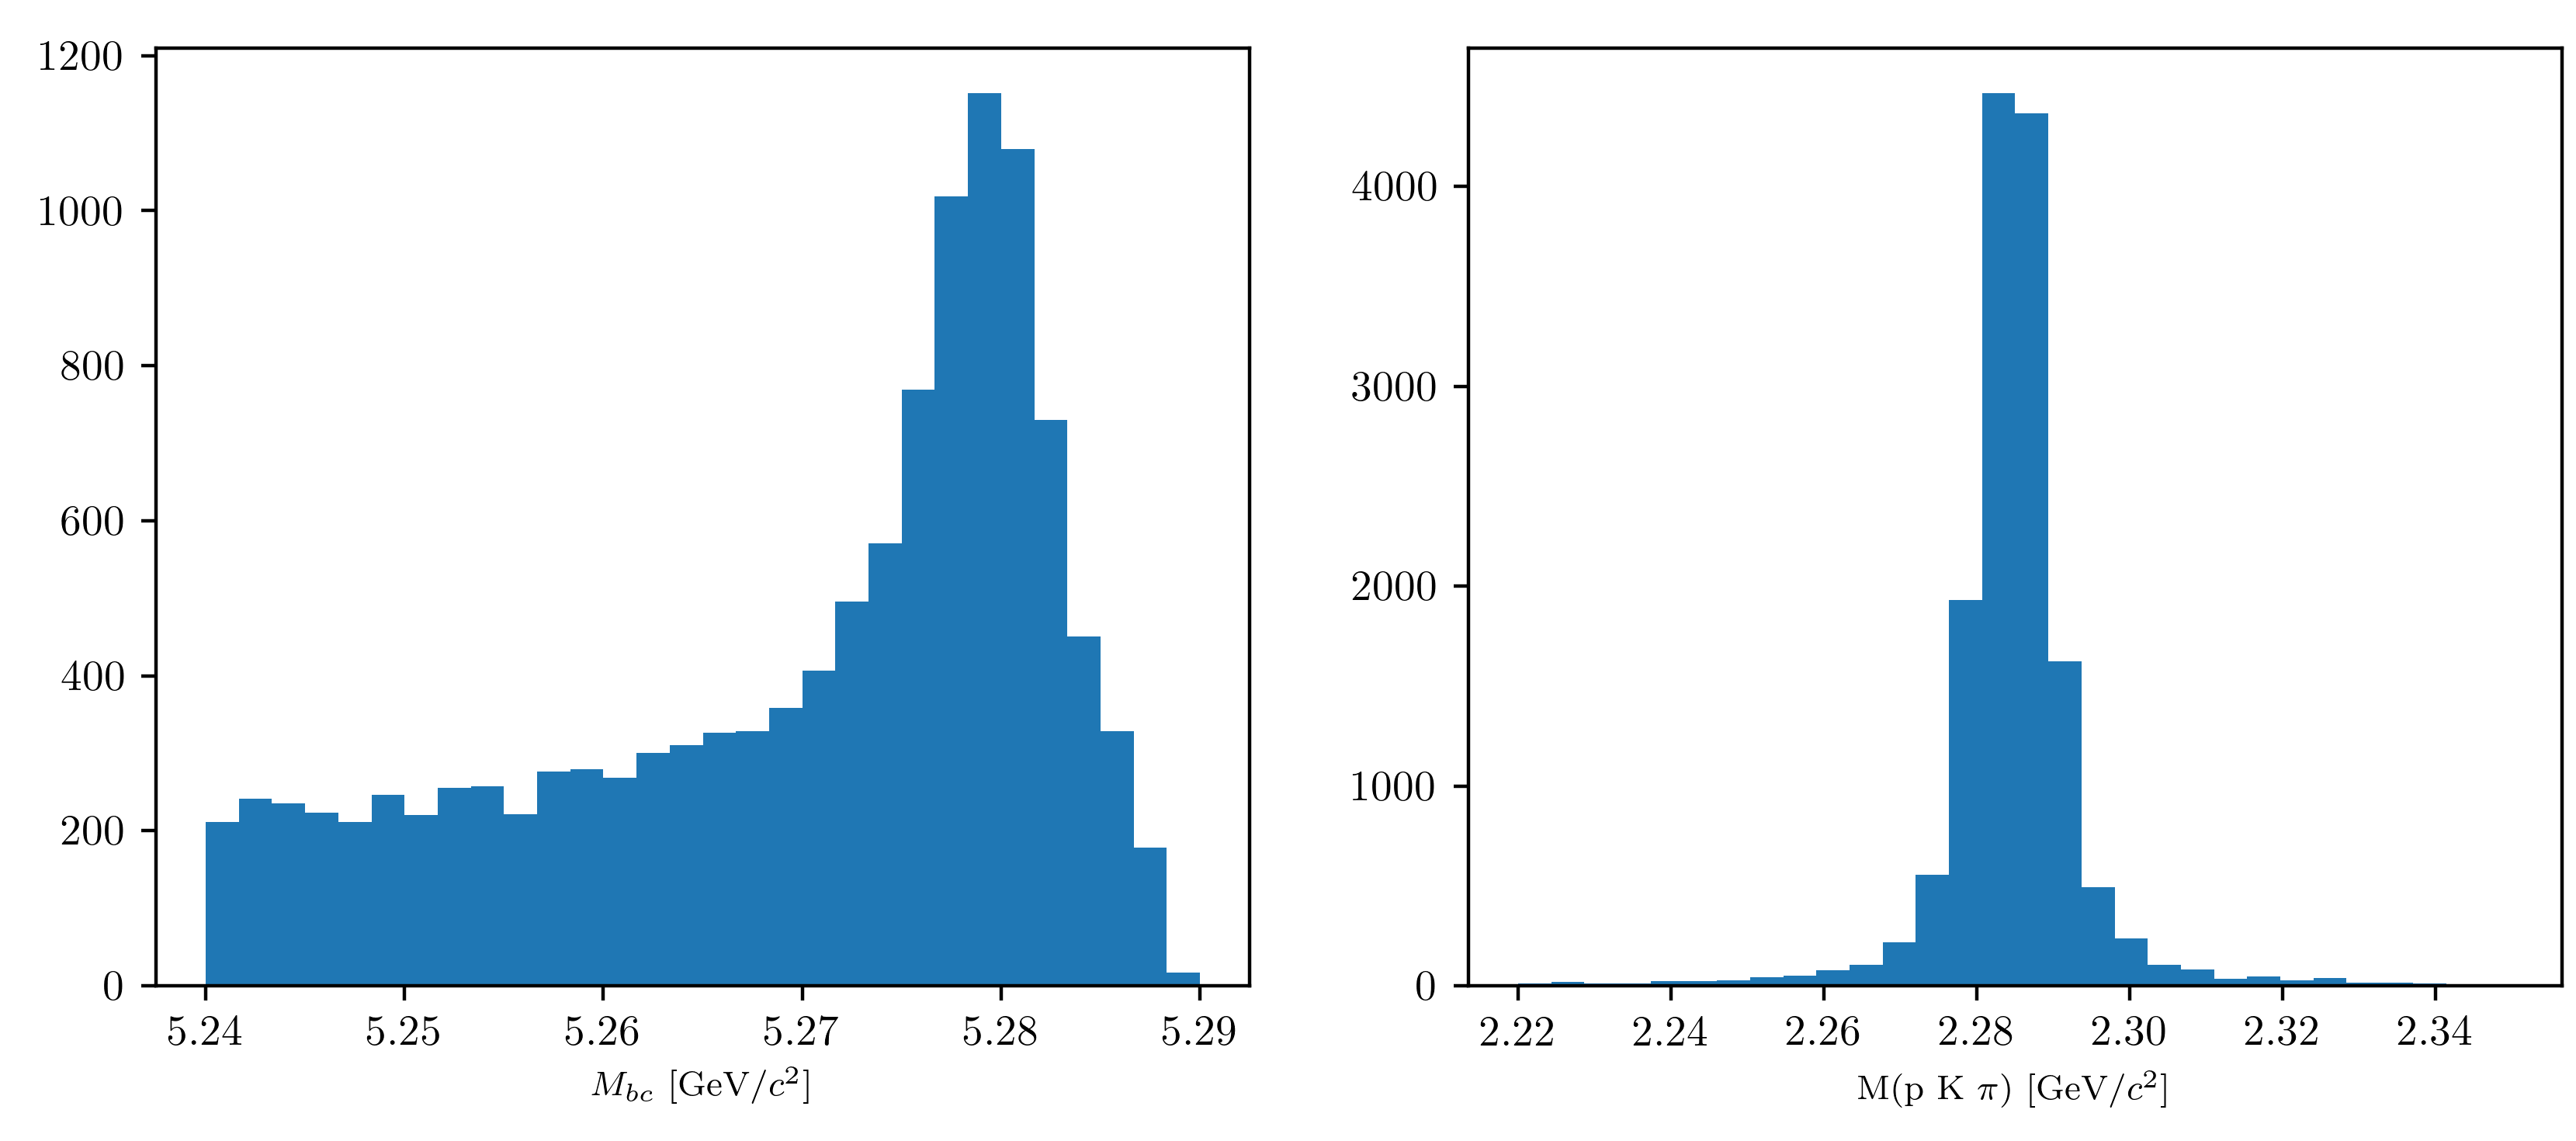
\includegraphics[width=1.0\textwidth]{03-Selection/figs/chargedBcorr_Mbc_MpKpi_TotalSignal.png}}
\caption{$M_{bc}$ and $M(p K \pi)$ distributions of $B_{tag}$ and $\Lambda_c$ candidates reconstructed in the signal sample.}
\label{fig:chargedBcorr_Mbc_MpKpi_TotalSignal}
\end{figure}

\subsection{Wrongly reconstructed $B_{tag}$ candidates}\label{wronglyBtag}

In the case of the signal sample the distributions for the beam-constrained mass $M_{bc}$ and for the correctly reconstructed $\Lambda_c$ candidates, look
like in \cref{fig:chargedBcorr_Mbc_MpKpi_TotalSignal}. If one then investigates the $M_{bc}$ distribution of the $B_{tag}$ candidates reconstructed with 
FEI, it can be seen that there is a peaking structure for wrongly reconstructed $B$ 
mesons (as in \cref{fig:wrongly_recoB}), according to the BASF2 internal truth matching variable \textbf{isSignal}.
It is obvious from this that the BASF2 internal truth matching variable cannot be used to separate properly the signal events in correctly and wrongly reconstructed $B$ mesons. In the study  BELLE2-NOTE-TE-2021-026 \url{https://docs.belle2.org/record/2711/files/BELLE2-NOTE-TE-2021-026.pdf} a possible solution was found developing new variables that can be used for an improved truth matching for the FEI (those variables were added to a newer BASF2 release than the one used for this study). In the present study instead a more "traditional" approach was adopted: fitting the $M_{bc}$ distribution with a sum of PDFs that account for the flat (background) component and the peaking (signal) component. The first component represents the combinatorial background, i.e. $B$ mesons that were mis-reconstructed, and therefore those events are denoted from now on as    "\textbf{misreconstructed signal}".  
The peaking component represents the correctly reconstructed signal events in $M_{bc}$ and therefore denoted from now on as "\textbf{reconstructed signal}".  Only the second one is then considered for the signal yield, while the first is counted as a background.
To validate this method a control decay study was performed on the flavor correlated $B^+ \rightarrow \bar{D^0}$ channel. 


\begin{figure}[h!]
\centering
{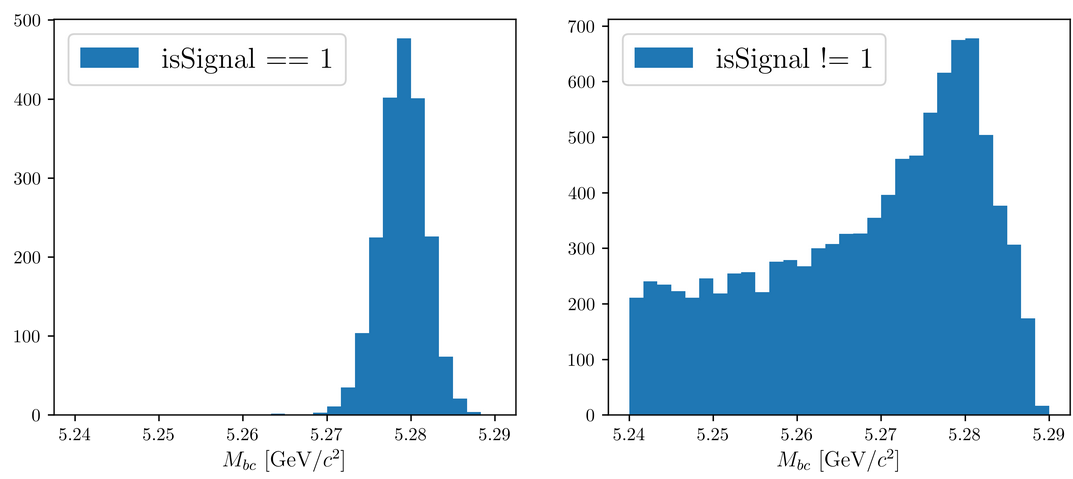
\includegraphics[width=1.\textwidth]{03-Selection/figs/wrongly_recoB.png}}
\caption{$M_{bc}$ distribution of $B_{tag}$ candidates reconstructed in the signal sample, truth-matched (on the left) and not (on the right).}
\label{fig:wrongly_recoB}
\end{figure}



\section{Signal selection optimization}

To further enhance the purity of the signal decays, an optimization procedure is adopted to determine optimal cuts for a set of variables for each decay mode under investigation by this study.
The cuts on the following variables are optimized:
\begin{itemize}
    \item $foxWolframR2$: the event based ratio
of the 2-nd to the 0-th order Fox-Wolfram moments
    \item SignalProbability: the already mentioned signal probability calculated by FEI using FastBDT
    \item $p^{\Lambda_c}_{CMS}$: momentum of the $\Lambda_c$ candidates in the center of mass system
\end{itemize}

The optimization is based on the Figure Of Merit (FOM): FOM = $\frac{S}{\sqrt{S+B}}$

Where S and B are respectively signal and background events in the signal region: $M_{bc} > $ 5.27 GeV/$c^2$,  2.2665  $< M(p K \pi) <$ 2.3065 GeV/$c^2$.\\
Due to the issue reported in Sec. \ref{wronglyBtag}, to separate signal events that peak in $M_{bc}$ from the ones that are not (which are then categorized as background events), the events reconstructed in the signal sample are fitted. with a sum of Crystal Ball function and Argus for each cut value on the corresponding variable to optimize (as in \cref{fig:wrongB_Mbc}).

\begin{figure}[h!]
%\centering
{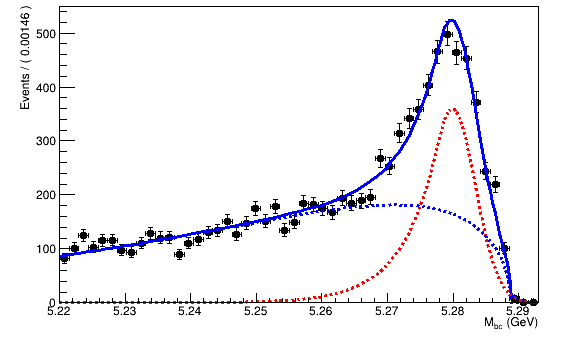
\includegraphics[width=0.75\textwidth]{03-Selection/figs/wrongB_Mbc.png}}
\caption{Example of a fit used to separate the correctly reconstructed $B$ mesons (described by the red dotted Crystal Ball function) from the wrongly reconstructed ones (described by the blue dotted Argus function).}
\label{fig:wrongB_Mbc}
\end{figure}


\chapter{2D simultaneous fit}


\label{sec:2DsimFit}
\section{Probability Density Functions (PDFs) for the two dimensional fit}\label{sec:2Dpdf}

The reconstructed events can be categorized as follows:
\begin{itemize}
    \item peaking in both $M_{bc}$ and $M$($p K \pi$ )
    \item peaking in $M_{bc}$ but not in $M$($p K \pi$ )
    \item peaking in $M$($p K \pi$) but not in $M_{bc}$
    \item flat in both $M_{bc}$ and $M$($p K \pi$ )
\end{itemize}

The first category is represented by the reconstructed signal: signal events which are correctly reconstructed. The signal events which are misreconstructed fall into the third category. The sum of the two is the so called "total signal".
The PDFs used to describe the total signal distributions are discussed first.

\subsection{Total Signal fits}
For all the decays, the final sample of total signal events presents a peak around the expected $B$ meson mass and a tail at low $M_{bc}$ values.

\begin{figure}
\centering

{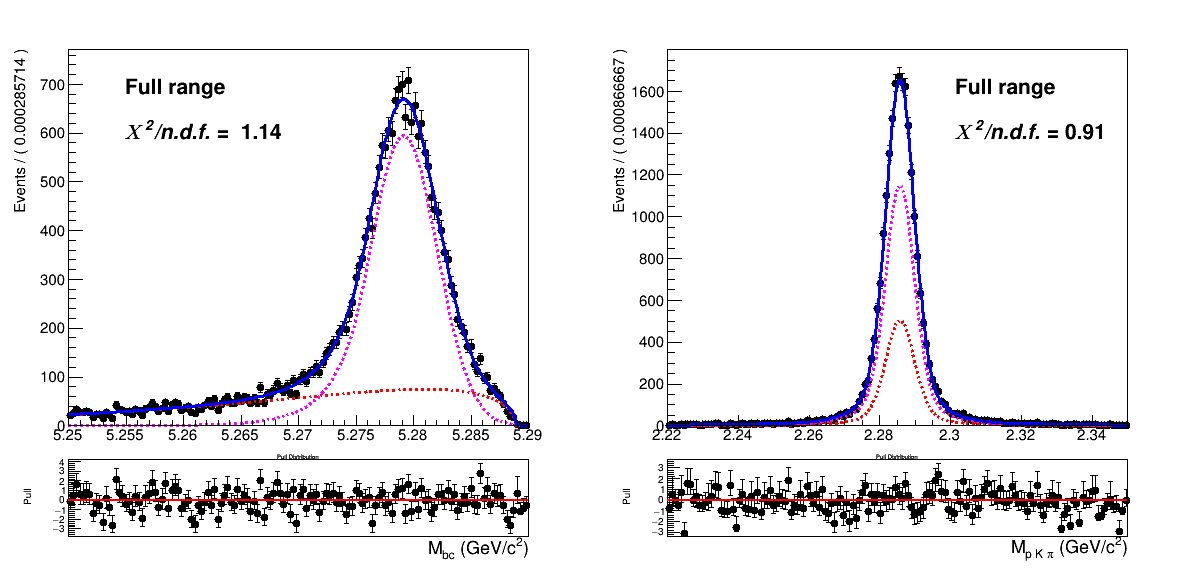
\includegraphics[width=0.7\textwidth]{04-SimultaneousFit/figs/5streams_TotalSignal_charged_corrLambdaC_2Dfit.png}}
\caption{Two dimensional fit of charged correlated total signal events in $M_{bc}$  and $M(p K \pi)$ }
\label{fig:5streams_TotalSignal_charged_corrLambdaC_2Dfit}
\end{figure}


    

\begin{figure}
\centering

{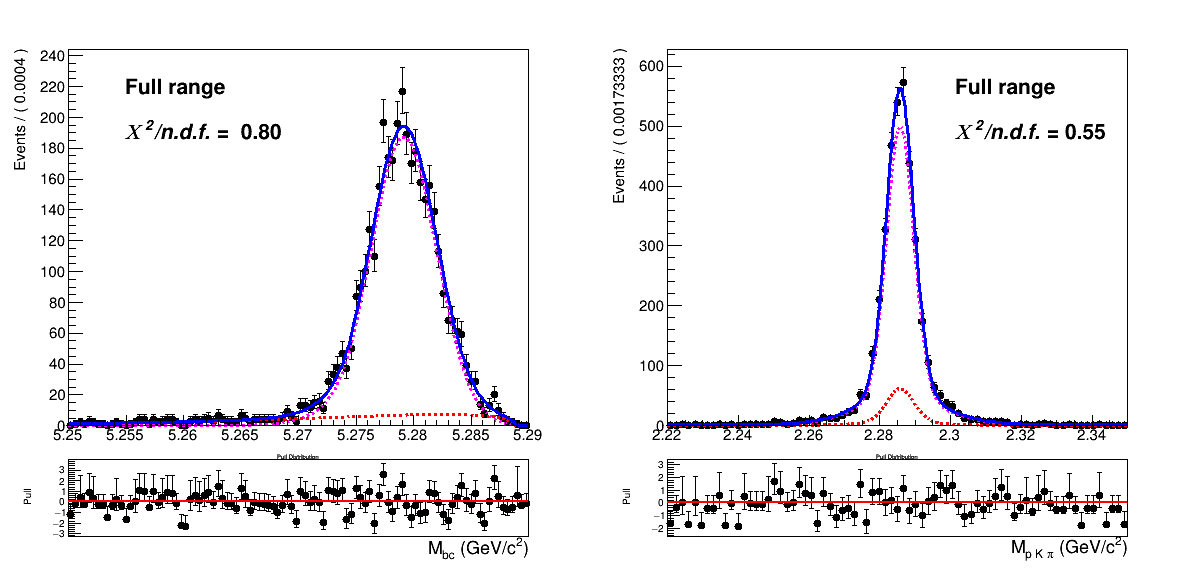
\includegraphics[width=0.7\textwidth]{04-SimultaneousFit/figs/stream12345_TotalSignal_charged_anticorrLambdaC_2Dfit.png}}
\caption{Two dimensional fit of charged anticorrelated total signal events in $M_{bc}$  and $M(p K \pi)$ }
\label{fig:5streams_TotalSignal_charged_anticorrLambdaC_2Dfit}
\end{figure}


\begin{figure}
\centering
{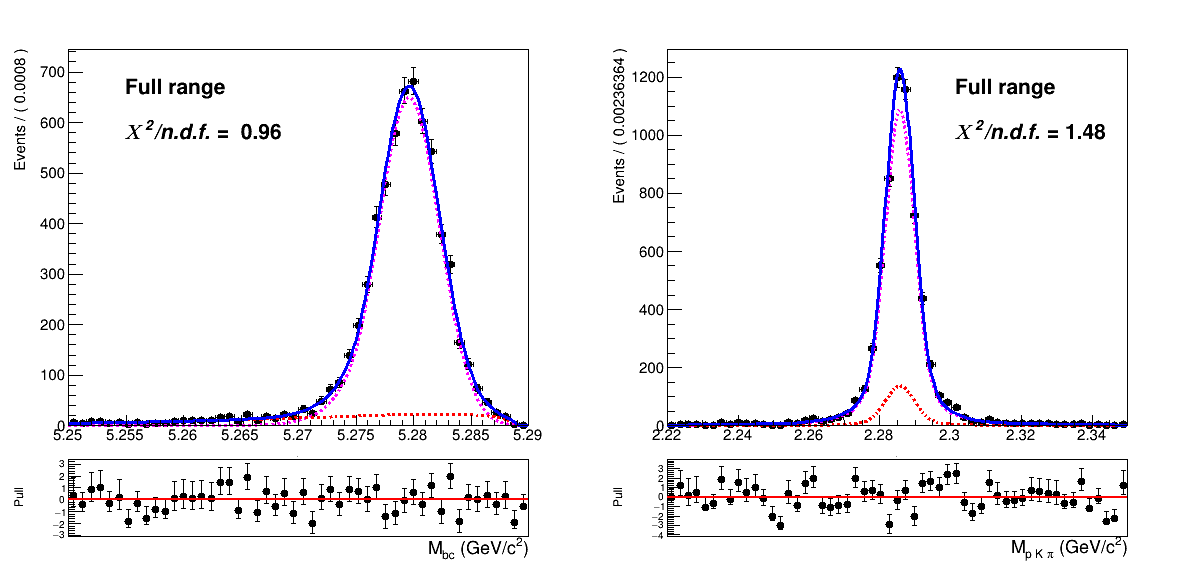
\includegraphics[width=0.7\textwidth]{04-SimultaneousFit/figs/NEWstream01234_TotalSignal_neutral_corrLambdaC_2Dfit.png}}
\caption{Two dimensional fit of neutral correlated total signal events in $M_{bc}$  and $M(p K \pi)$ }
\label{fig:5streams_TotalSignal_neutral_corrLambdaC_2Dfit}
\end{figure}

\begin{figure}
\centering
{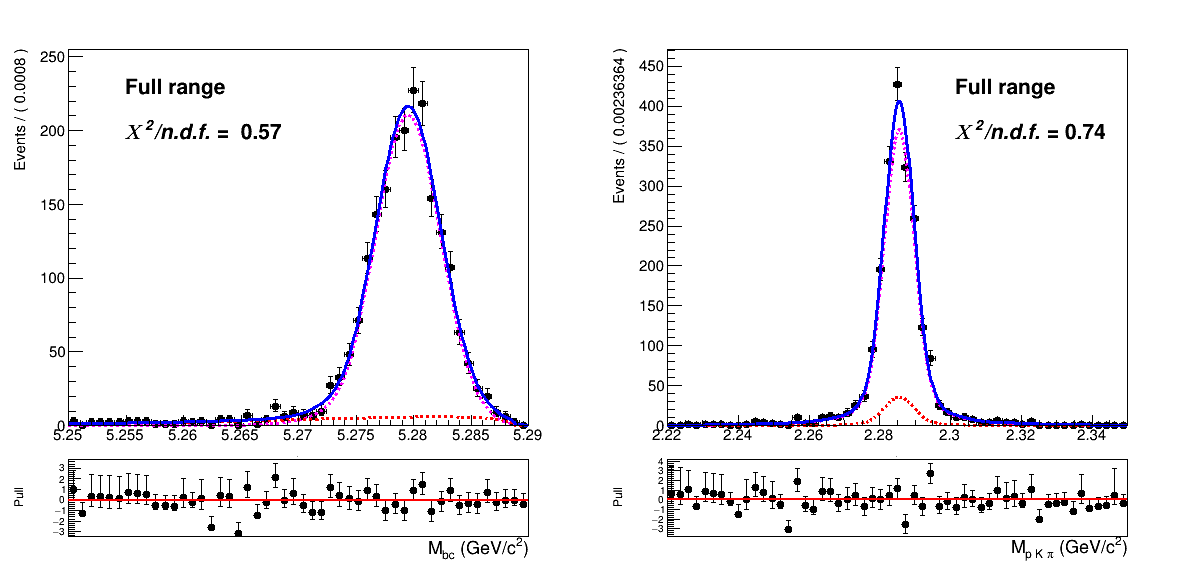
\includegraphics[width=0.7\textwidth]{04-SimultaneousFit/figs/NEWstream01234_TotalSignal_neutral_anticorrLambdaC_2Dfit.png}}
\caption{Two dimensional fit of neutral anticorrelated total signal events in $M_{bc}$  and $M(p K \pi)$ }
\label{fig:5streams_TotalSignal_neutral_anticorrLambdaC_2Dfit}
\end{figure}
\newpage
The 2D fits shown above are  performed on five streams of signal MC with a sum of the following probability density functions:
\vspace{0.2 cm}
 \begin{equation}
        P^{recSig}_{B,\Lambda_c}(M_{bc}, M(p K \pi)) = \Gamma_{CB}(M_{bc}) \times \rho_G(M(p K \pi))
    \label{eq:RecSigEq}
\end{equation} 
\begin{equation}
        P^{misSig}_{B,\Lambda_c}(M_{bc}, M(p K \pi)) = \Gamma_{ARG}(M_{bc}) \times \rho_G(M(p K \pi))
    \end{equation}  \label{eq:MisSigEq}

The first is used to fit the reconstructed signal and $\Gamma_{CB}(M_{bc})$ is a Crystal Ball function. The second is used to model the misreconstructed signal and $\Gamma_{ARG}(M_{bc})$ is an Argus function. In both cases a sum of three Gaussian functions $\rho_G(M(p K \pi))$ describes the mass of the $\Lambda_c$ baryon.  


As already said, only the events of reconstructed signal are considered as signal, while the misreconstructed signal is considered as background.

\subsection{Mbc peaking and flat background}

The background composed of $B\bar{B}$ events where no $\Lambda_c$ baryon  is produced, is flat in its invariant mass, but  can be distinguished in the following two categories:

\begin{itemize}
    \item peaking in $M_{bc}$ but not in $M$($p K \pi$)
    \item flat in both $M_{bc}$ and $M$($p K \pi$ )
\end{itemize}

as one can see in the following plots.

\begin{figure}
\centering
{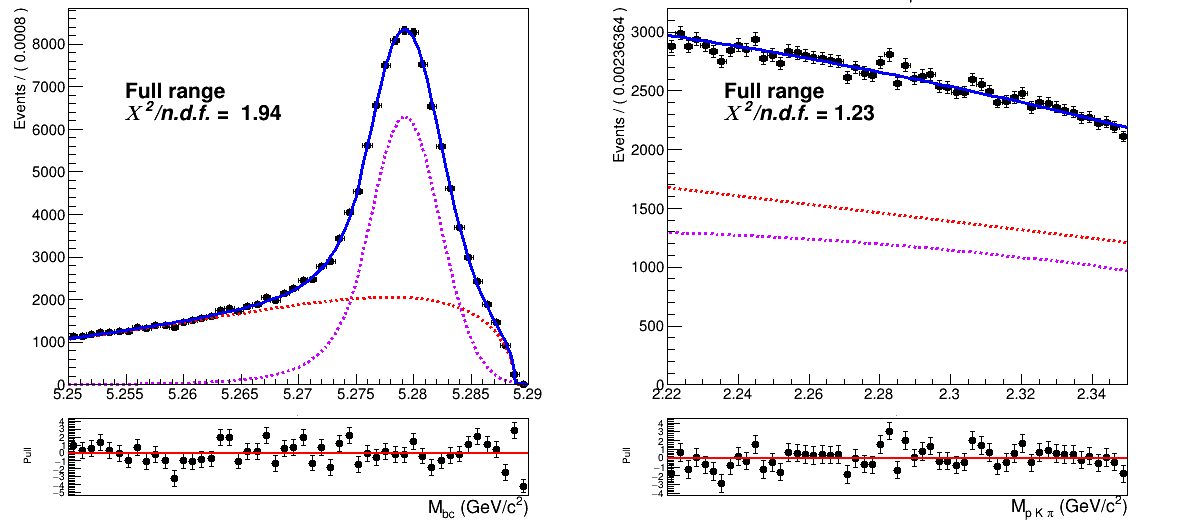
\includegraphics[width=0.7\textwidth]{04-SimultaneousFit/figs/stream01234_charged_corrLambdaC_TotalGeneric_2DFit_onlyArgus.png}}
\caption{Two dimensional fit of charged correlated $B\bar{B}$  events in $M_{bc}$  and $M(p K \pi)$ }
\label{fig:stream01234_charged_corrLambdaC_TotalGeneric_2DFit}
\end{figure}


\begin{figure}
\centering
{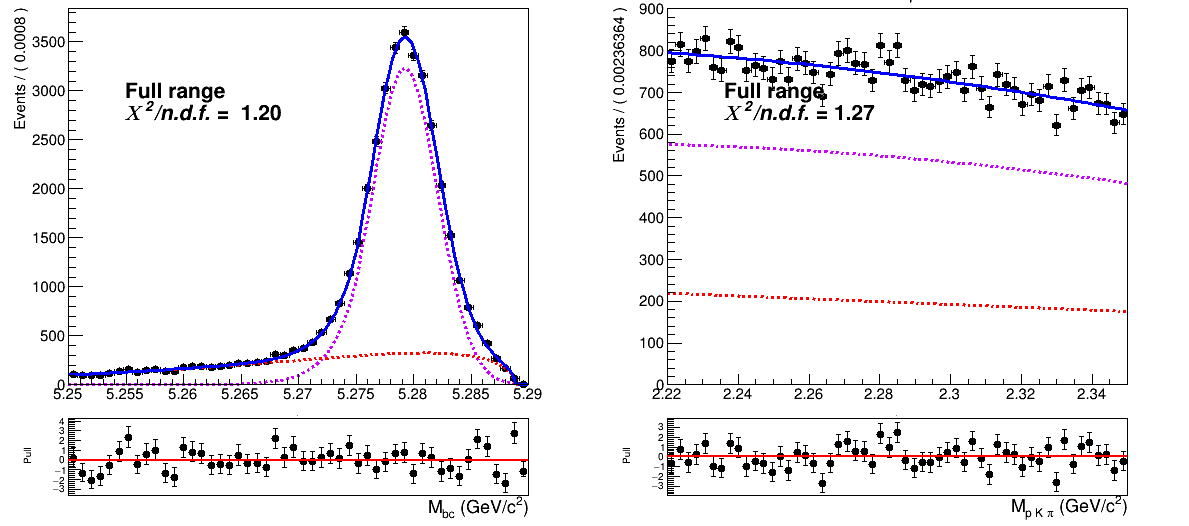
\includegraphics[width=0.7\textwidth]{04-SimultaneousFit/figs/stream12345_charged_anticorrLambdaC_TotalGeneric_2DFit_only_argus.png}}
\caption{Two dimensional fit of charged anticorrelated $B\bar{B}$  events in $M_{bc}$  and $M(p K \pi)$ }
\label{fig:stream12345_charged_anticorrLambdaC_TotalGeneric_2DFit}
\end{figure}

\begin{figure}
\centering
{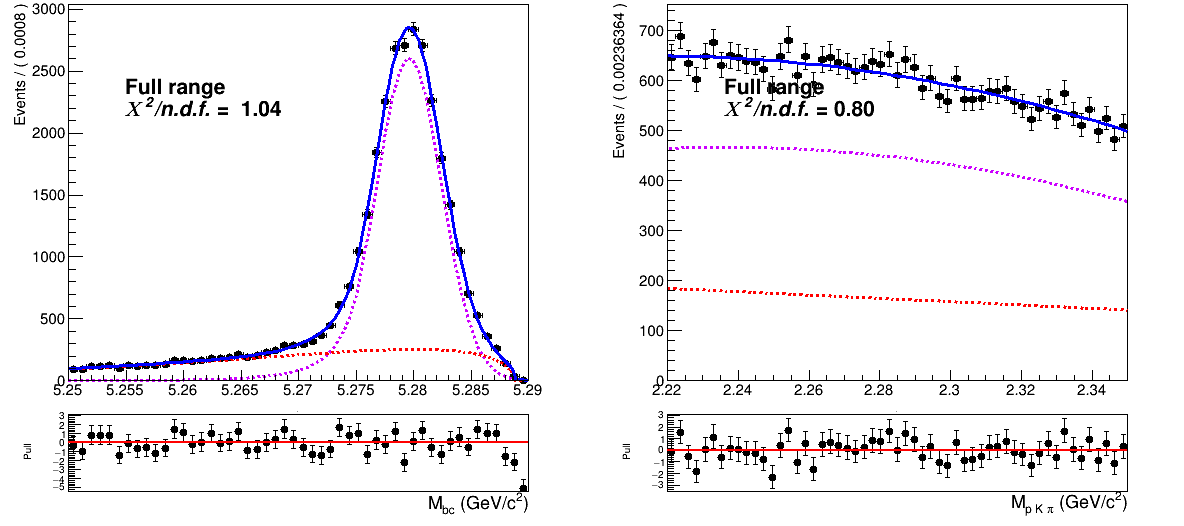
\includegraphics[width=0.7\textwidth]{04-SimultaneousFit/figs/stream01245_neutral_corrLambdaC_TotalGeneric_2DFit.png}}
\caption{Two dimensional fit of neutral correlated $B\bar{B}$  events in $M_{bc}$  and $M(p K \pi)$ }
\label{fig:stream01245_neutral_corrLambdaC_TotalGeneric_2DFit}
\end{figure}

\begin{figure}
\centering
{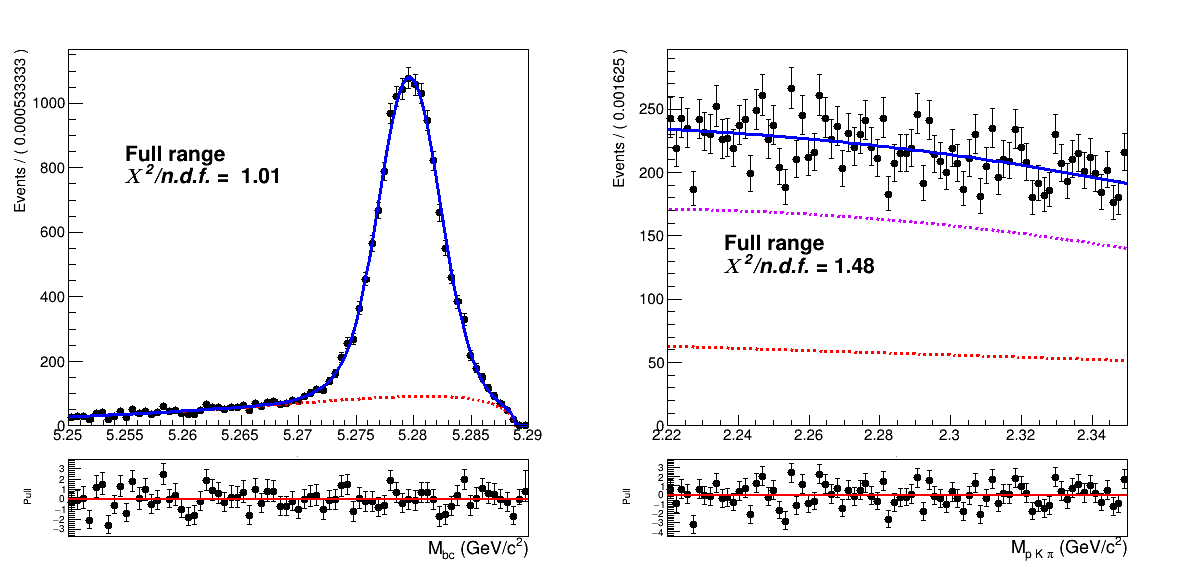
\includegraphics[width=0.7\textwidth]{04-SimultaneousFit/figs/stream01235_neutral_anticorrLambdaC_Generic_2DFit.png}}
\caption{Two dimensional fit of neutral anticorrelated $B\bar{B}$  events in $M_{bc}$  and $M(p K \pi)$ }
\label{fig:stream01235_neutral_anticorrLambdaC_Generic_2DFit}
\end{figure}


\newpage
This background presents a 
similar shape of the distribution in $M_{bc}$: the probability
density functions used for it are again a  Crystal Ball and an Argus. \\
The two types of background (peaking/flat in $M_{bc}$) are described by:
\begin{equation}
P^{peaking}_{B,\Lambda_c}(M_{bc}, M(p K \pi)) = \Gamma_{CB}(M_{bc})  \times \rho_{Cheb(a0,a 1)}(M(p K \pi))
\end{equation}

\begin{equation}
P^{flat}_{B,\Lambda_c}(M_{bc}, M(p K \pi)) =  \Gamma_{ARG}(M_{bc}) \times \rho_{Cheb(b0)}(M(p K \pi))
\end{equation}
\newline
%\vspace{0.5 cm}
where $\rho_{Cheb(a0,a 1)}(M(p K \pi))$ and $\rho_{Cheb(b0)}(M(p K \pi))$  represent a second order and first order Chebychev polynomial function respectively.

\subsection{Crossfeed background}
The contamination of misreconstructed $B^0 \rightarrow \Lambda_c$ events in the $B^+$ signal (and vice-versa) induces a background  peaking in $M(p K \pi)$, but it also slightly peaks near the $B$ meson mass, as one can see in Fig. \ref{fig:chargedBcorr_CrossfeedLambdaCpeak}
\newpage
\begin{figure}
\centering
{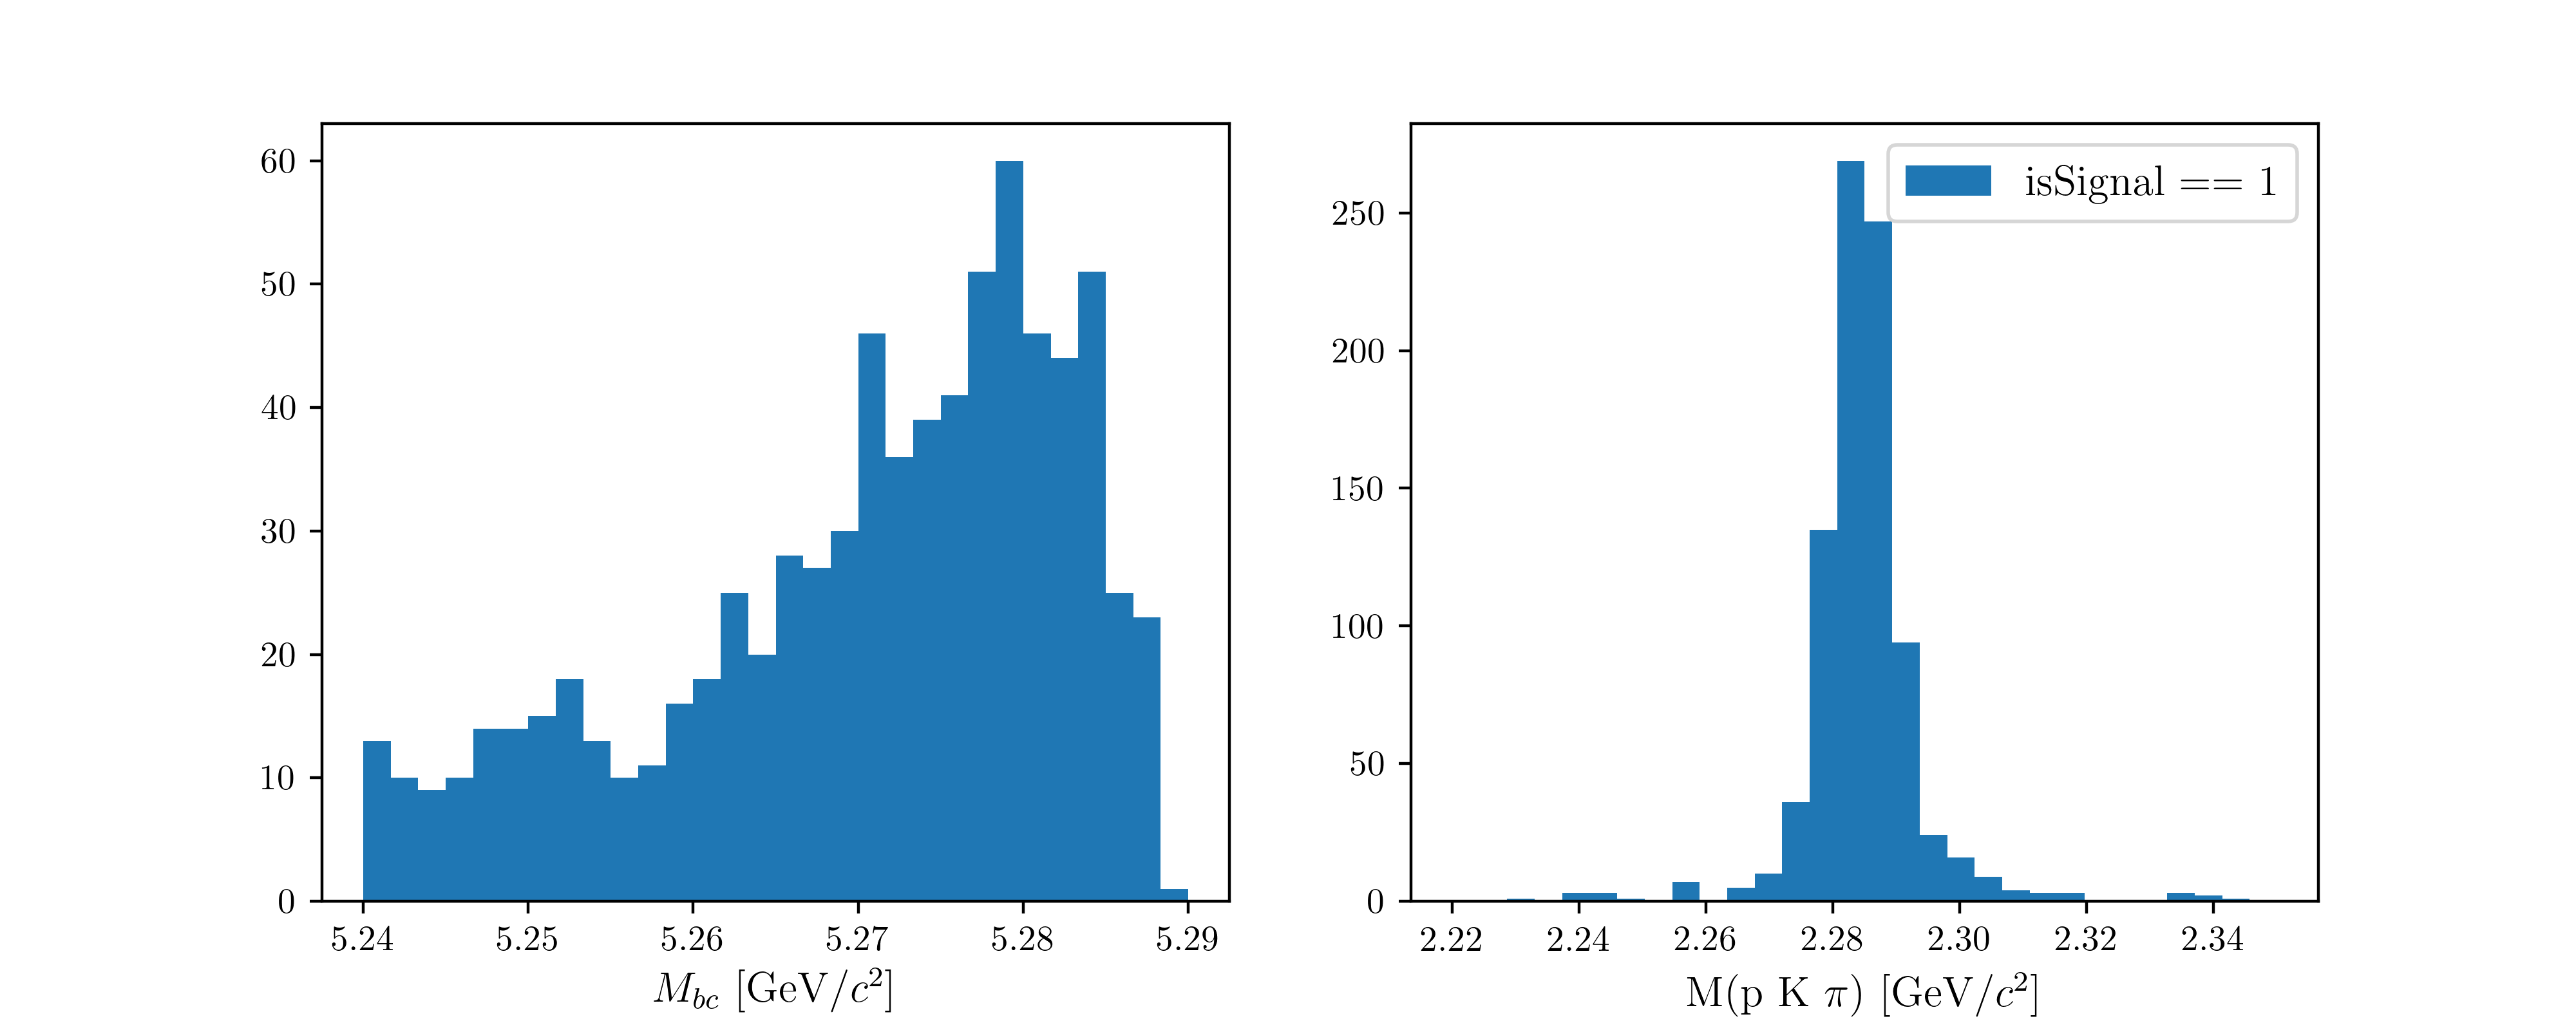
\includegraphics[width=0.8\textwidth]{04-SimultaneousFit/figs/chargedBcorr_CrossfeedLambdaCpeak.png}}
\caption{Crossfeed distribution in $M_{bc}$  and $M(p K \pi)$ }
\label{fig:chargedBcorr_CrossfeedLambdaCpeak}
\end{figure}


\begin{figure}
\centering
{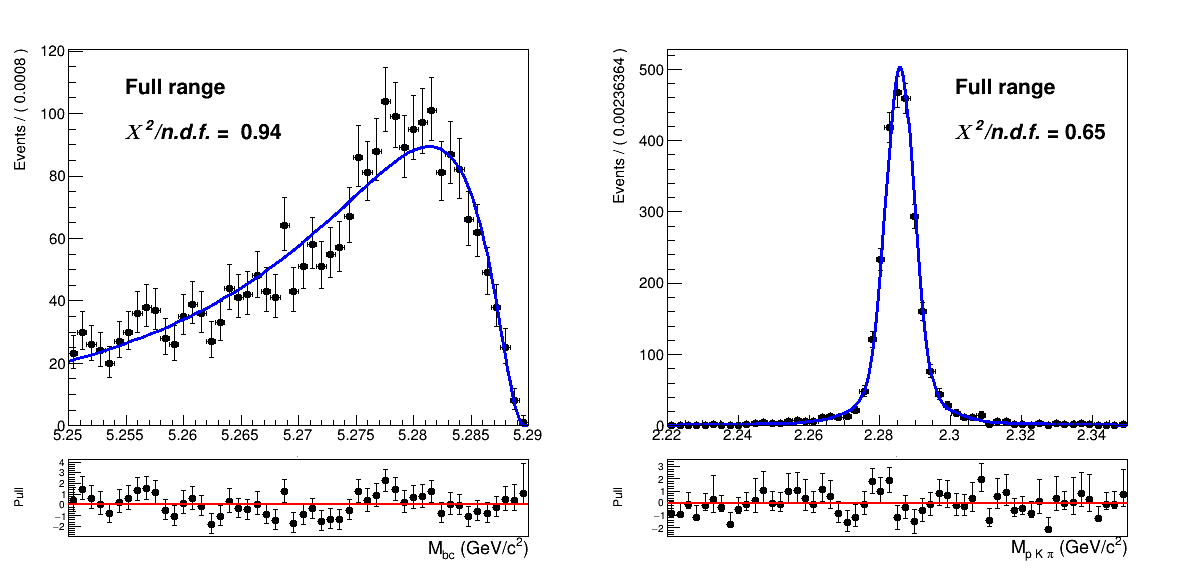
\includegraphics[width=0.7\textwidth]{04-SimultaneousFit/figs/streams01245_CrossfeedPeak_charged_corrLambdaC_2Dfit.png}}
\caption{Two dimensional fit of crossfeed events in charged correlated channel in $M_{bc}$  and $M(p K \pi)$ }
\label{fig:streams01245_CrossfeedPeak_charged_corrLambdaC_2Dfit}
\end{figure}


\begin{figure}
\centering
{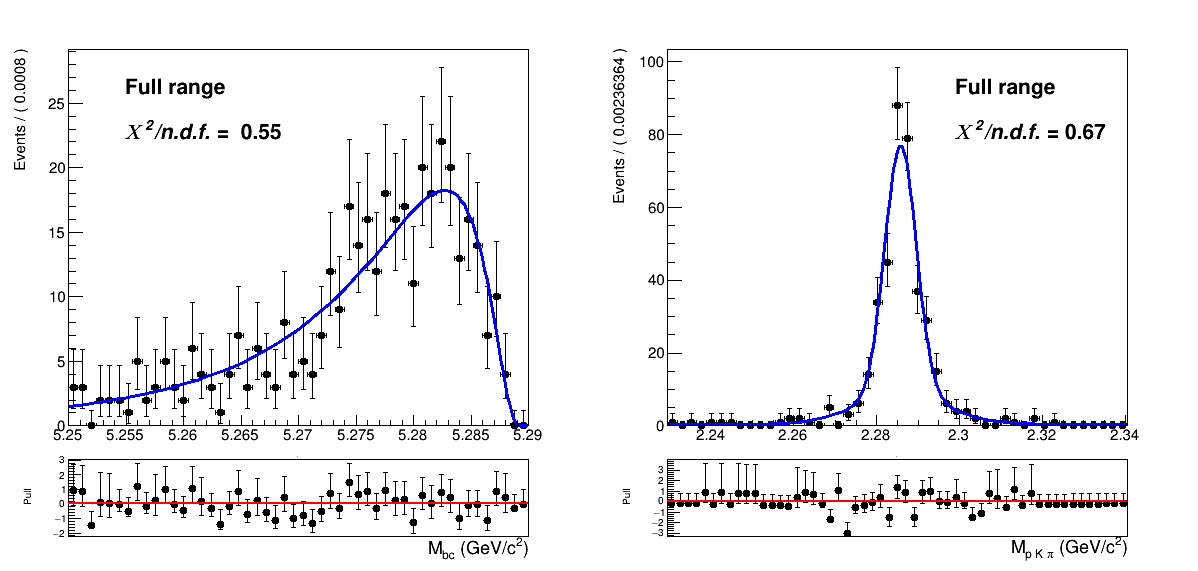
\includegraphics[width=0.7\textwidth]{04-SimultaneousFit/figs/streams01234_CrossfeedPeak_charged_anticorr_LambdaC_2Dfit.png}}
\caption{Two dimensional fit of crossfeed events in charged anticorrelated channel in $M_{bc}$  and $M(p K \pi)$ }
\label{fig:streams01234_CrossfeedPeak_charged_anticorr_LambdaC_2Dfit}
\end{figure}

\begin{figure}
\centering
{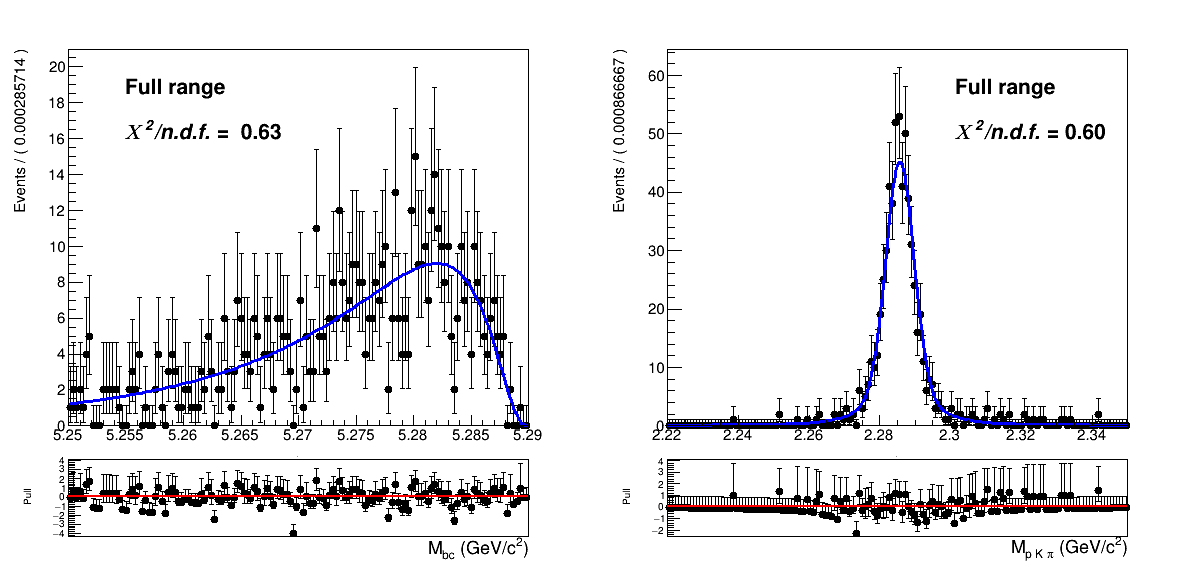
\includegraphics[width=0.7\textwidth]{04-SimultaneousFit/figs/streams01234_CrossfeedPeak_neutral_corrLambdaC_2Dfit.png}}
\caption{Two dimensional fit of crossfeed events in neutral correlated channel in $M_{bc}$  and $M(p K \pi)$ }
\label{fig:streams01234_CrossfeedPeak_neutral_corrLambdaC_2Dfit}
\end{figure}

\begin{figure}
\centering
{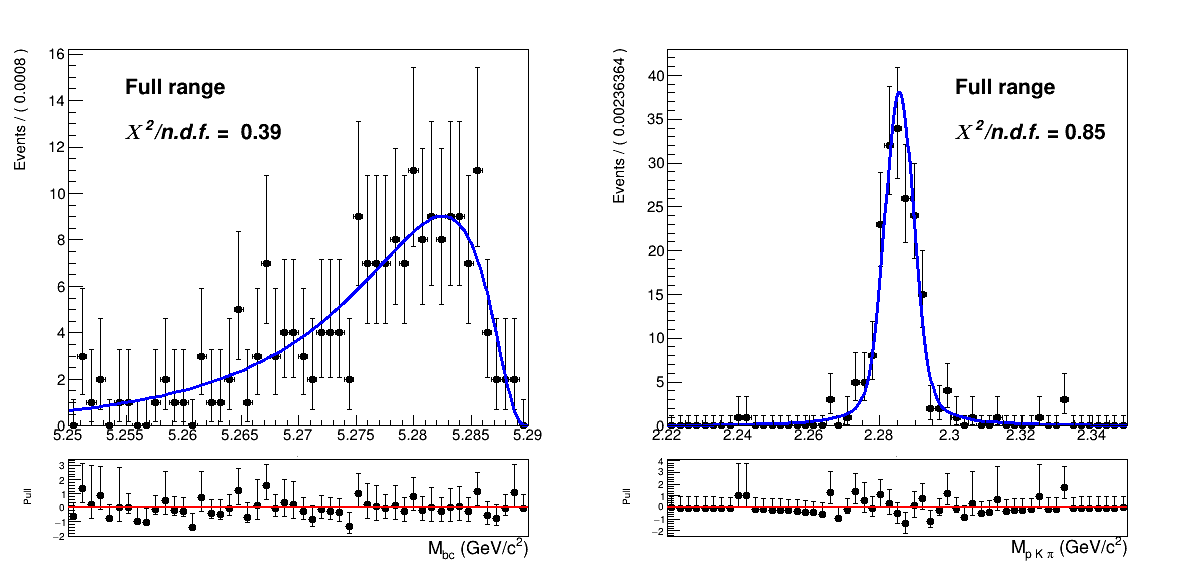
\includegraphics[width=0.7\textwidth]{04-SimultaneousFit/figs/stream12345_Crossfeed_neutral_anticorrLambdaC_2Dfit.png}}
\caption{Two dimensional fit of crossfeed events in neutral anticorrelated channel in $M_{bc}$  and $M(p K \pi)$ }
\label{fig:stream12345_Crossfeed_neutral_anticorrLambdaC_2Dfit}
\end{figure}

\newpage
The 2D fit shown above are  performed on five streams of signal MC with a sum of the following probability density function:
\vspace{0.2 cm}
 \begin{equation}
        P^{Crossfeed}_{B,\Lambda_c}(M_{bc}, M(p K \pi)) = \Gamma_{Novosibirsk}(M_{bc}) \times \rho_G(M(p K \pi))
    %\label{eq:}
\end{equation} 

where $\Gamma_{Novosibirsk}(M_{bc})$ is a Novosibirsk function and the mass of the $\Lambda_c$ baryon is described by the same sum of three Gaussian functions $\rho_G(M(p K \pi))$ as in Eq.\ref{eq:RecSigEq}.

\subsection{Continuum background}


 Besides the dataset recorded at the energy of the $\Upsilon(4S) $ resonance  ($E^{on-res}
_{CMS} = $ 10.58 GeV), the \textit{Belle} experiment recorded a sample of 89.4 $fb^{-1}$ at an energy 60 MeV below the nominal  $\Upsilon(4S) $ resonance ($E^{off-res}_{CMS} = $ 10.52 GeV). The dataset allows to check for an appropriate modeling of the continuum MC simulation. %, by comparing the off-resonance data with the MC expectation for the continuum background. 
Using the official tables \newline ( \url{https://belle.kek.jp/secured/nbb/nbb.html}) the off-resonance sample is scaled by 

\begin{equation}
    \frac{\mathcal{L}^{on-res}}{\mathcal{L}^{off-res}} \left( \frac{E^{off-res}_{CMS}}{E^{on-res}_{CMS}}\right)^2
\label{eq:off-resScaling}
\end{equation}


\noindent taking into account the difference in luminosity and in $E_{CMS}$ (Energy in center of mass system).


\begin{figure}[h!]
%\centering
{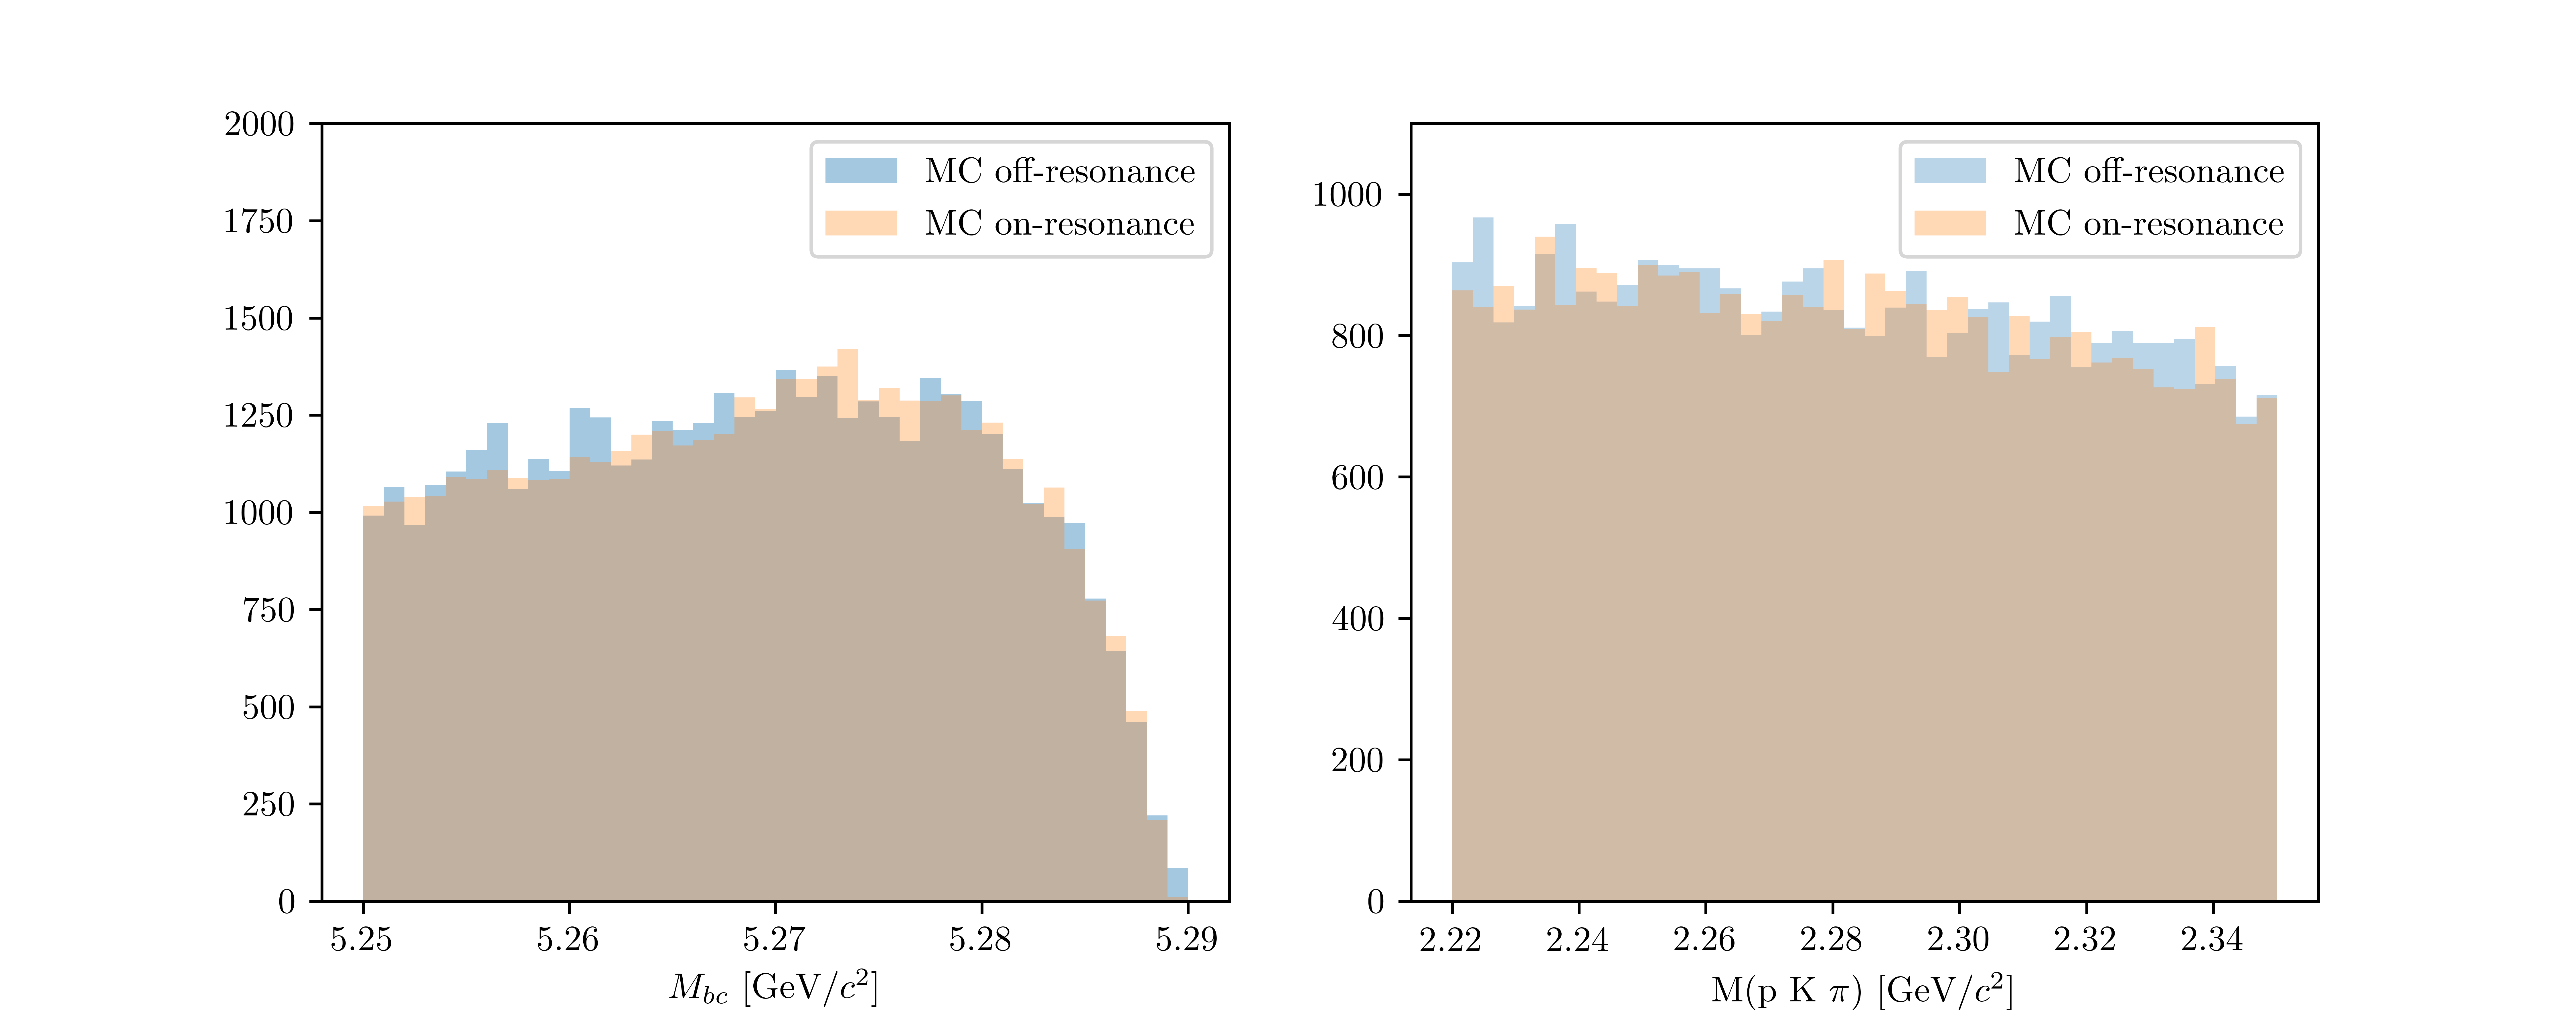
\includegraphics[width=1.05\textwidth]{04-SimultaneousFit/figs/MbcInvM_MC_on_off-resonance_comparison.png}}
\caption{$M_{bc}$ and $M(p K \pi)$ comparison between  on-/off-resonance (scaled) Monte Carlo simulated continuum. The scaling is applied according to \cref{eq:off-resScaling} and shifting the $M_{bc}$ distribution by $E^{on-res}_{CMS} - E^{off-res}_{CMS}$. }
\label{fig:MbcInvM_MC_on_off-resonance_comparison}
\end{figure} 

\noindent The plot in Fig.\ref{fig:MbcInvM_MC_on_off-resonance_comparison} shows the $M_{bc}$ and $M(p K \pi)$ distributions in the MC on-/off-resonance continuum after the scaling\footnote{it is obtained with the MC off-resonance sample being composed of 6 streams: the total amount is normalized}.

Ideally, provided that there's a good agreement between MC and data for the off-resonance sample and also between the MC  on-/off-resonance continuum after the scaling, one could directly use the scaled off-resonance data to describe the continuum background in the fit on data. There are two reasons that prevent this very straightforward approach:
\begin{itemize}

\item First, since the off-resonance MC (and data) present very low statistics (Fig. \ref{fig:off-resData_charged_corrLambdaC_InvM} shows the  $\Lambda_c$ 
invariant mass in off-resonance data), scaling them with all the applied selection cuts would cause the PDF describing the continuum to be very much affected by statistical fluctuations. 
\item Secondly, the $B$ meson candidates are reconstructed in both on-resonance and off-resonance events for values of $M_{bc} \geq 5.22 $ GeV/c$^2$, but the $E_{CMS}$ differs: there can be effects of correlations between the applied \textit{SignalProbability} cut and the $M_{bc}$ variable that one needs to take into account. %This effects on the $M_{bc}$ are carefully studied in the analysis of the control sample. 
\end{itemize}


\begin{figure}
\centering
\subcaptionbox{\label{fig:off-resData_charged_corrLambdaC_InvM}}
{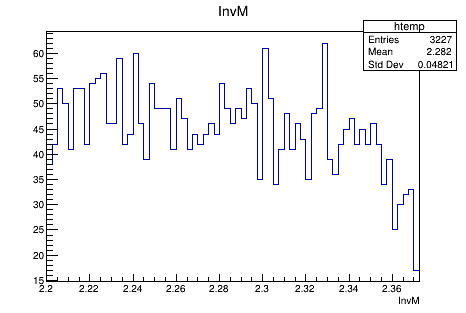
\includegraphics[width=.45\textwidth]{04-SimultaneousFit/figs/chargedCorrLambdaC_off-resData.png}}\quad
\subcaptionbox{\label{fig:off-resData_charged_corrLambdaC_InvM_woCS}}
{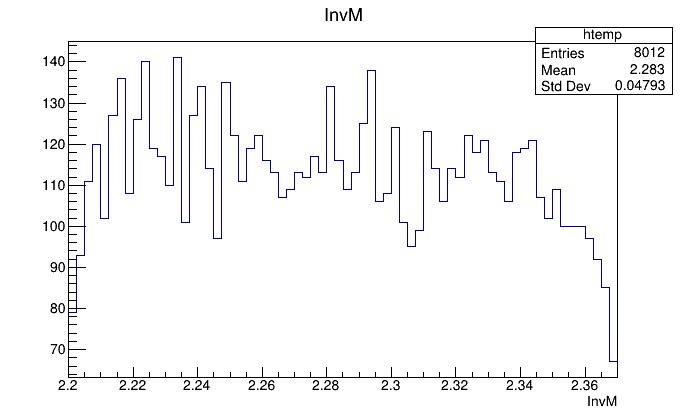
\includegraphics[width=.48\textwidth]{04-SimultaneousFit/figs/chargedCorrLambdaC_off-resData_woCScuts.png}} \quad
\caption{On the left: $\Lambda_c$ invariant mass in off-resonance data (all nominal cuts applied). On the right: $\Lambda_c$ invariant mass in off-resonance data after the continuum suppression cut removal.}
\end{figure}


\begin{figure}[H]
%\centering
{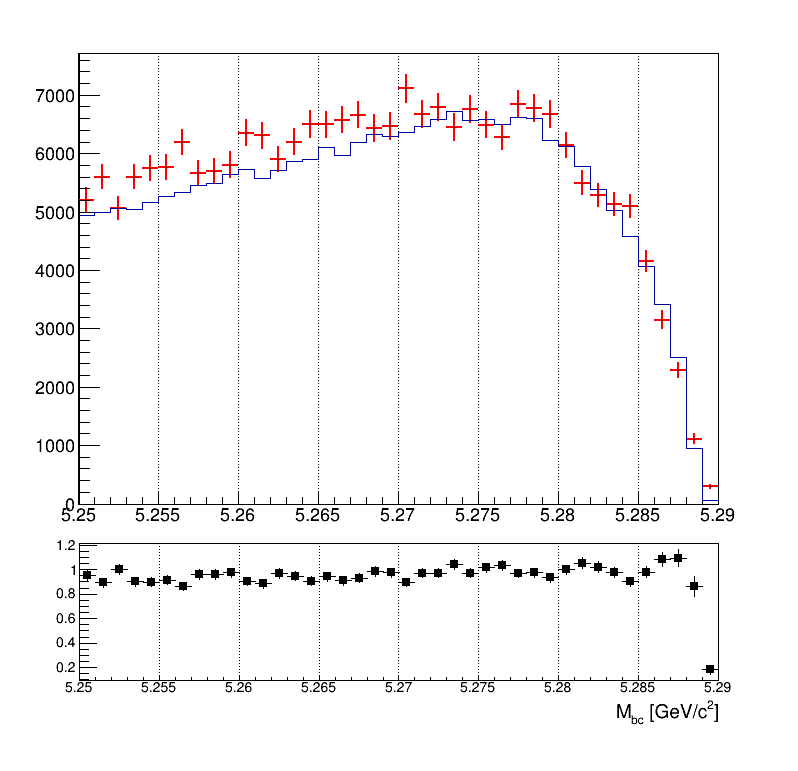
\includegraphics[width=0.5\textwidth]{04-SimultaneousFit/figs/stream01234_Mbc_continuumRescaling.png}}
\caption{$M_{bc}$ distributions of the MC (scaled) off-resonance sample (in red) and on-resonance (in blue) using 5 streams statistics and all nominal selection cuts applied.}
\label{fig:charged_corrLambdaC_Mbc_on_offResScaled}
\end{figure}

In Fig. \ref{fig:charged_corrLambdaC_Mbc_on_offResScaled} one can notice some discrepancy in the shapes, apart from the not negligible statistical fluctuations in the (scaled) off-resonance distribution.  



\newpage


\begin{figure}
\centering
\subcaptionbox{\label{fig:onRes_offResScaledMbc_corrLambdaC}}
{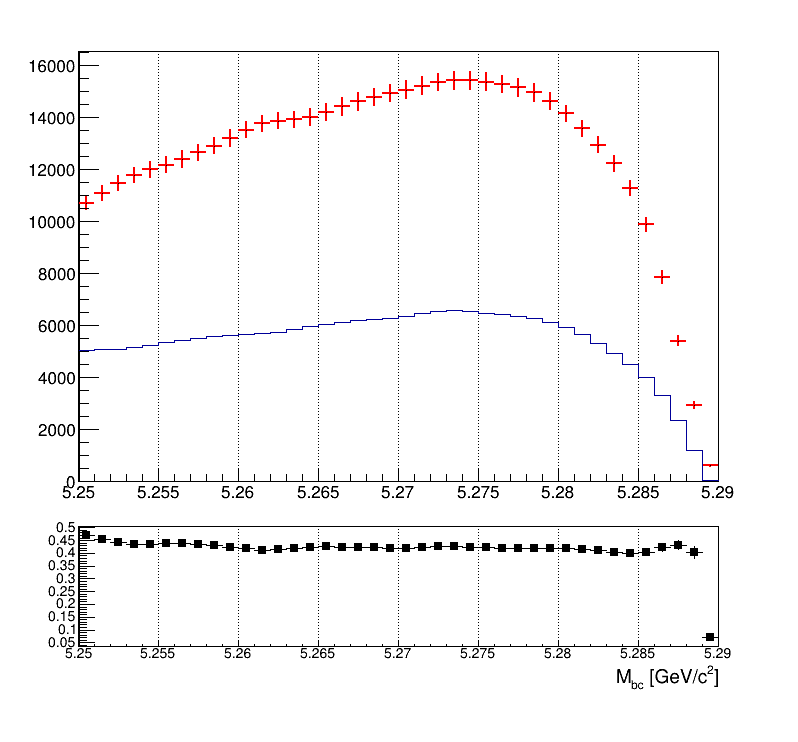
\includegraphics[width=.46\textwidth]{04-SimultaneousFit/figs/stream01235_charged_corrLambdaC_woCScuts_Mbc_scaling.png}} \quad
\subcaptionbox{\label{fig:Mbc_scaled_bin_correctedOffResContinuum}}
{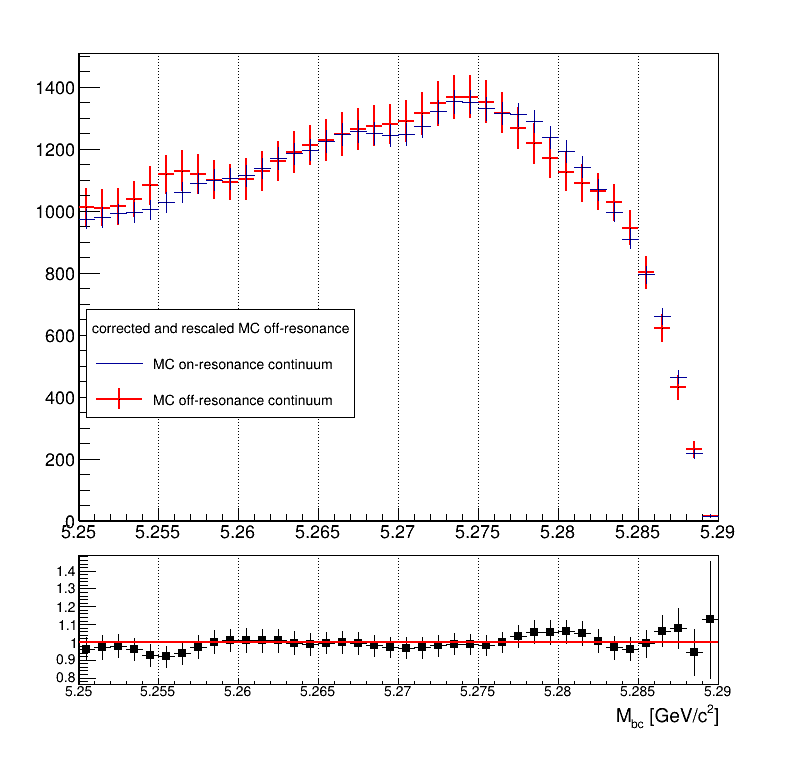
\includegraphics[width=.44\textwidth]{04-SimultaneousFit/figs/MC_on_off_resonance_stream4_continuum_2D_Mbc_corrected.png}} \quad
\caption{On the left: $M_{bc}$ distributions of the MC off-resonance sample without continuum suppression and the MC continuum sample with applied continuum suppression. On the right: $M_{bc}$ distributions of the corrected scaled MC off-resonance and on-resonance MC continuum.}
\end{figure}


The procedure adopted to obtain the PDF describing the continuum background  $M_{bc}$ distribution is the following:
\begin{itemize}

\item 5 streams of off-resonance MC were scaled according to \cref{eq:off-resScaling} without continuum suppression being applied and compared to the distribution of 5 streams of on-resonance continuum
\item From a ratio plot, like the one in Fig. \ref{fig:onRes_offResScaledMbc_corrLambdaC}, the bin-correction is obtained to correct the off-resonance data in the scaling procedure.
To obtain the shape that can describe the continuum background  $M_{bc}$ distribution on data the continuum suppression is not applied on the off-resonance continuum sample, in order to acquire more statistics. 
\end{itemize}

\noindent This procedure is first tested on an independent MC sample (see Fig. \ref{fig:Mbc_scaled_bin_correctedOffResContinuum} ) to check the result on simulated data before applying it on data.



\begin{figure}[H]
\centering
\subcaptionbox{\label{fig:corrLambdaC_OffResonance_w_wo_CS_comparison_5streams}}
{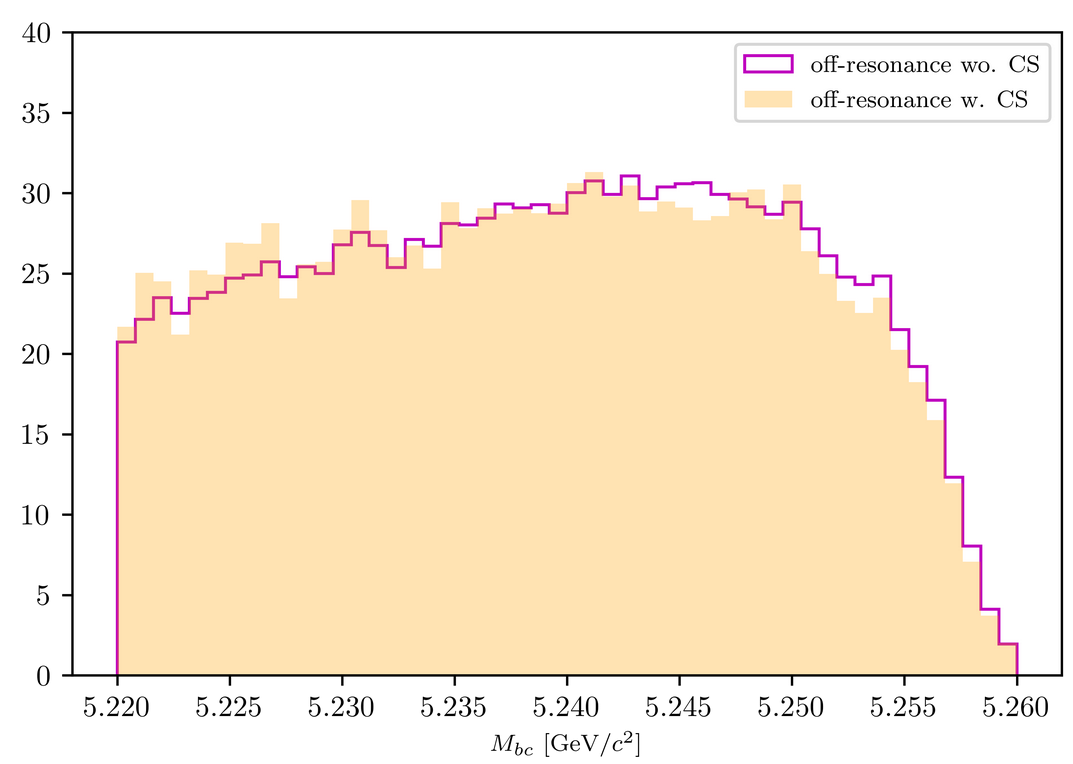
\includegraphics[width=.65\textwidth]{04-SimultaneousFit/figs/corrLambdaC_OffResonance_w_wo_CS_comparison_5streams.png}} 
\subcaptionbox{\label{fig:corrLambdaC_OffResonance_w_wo_CS_comparison_Data}}
{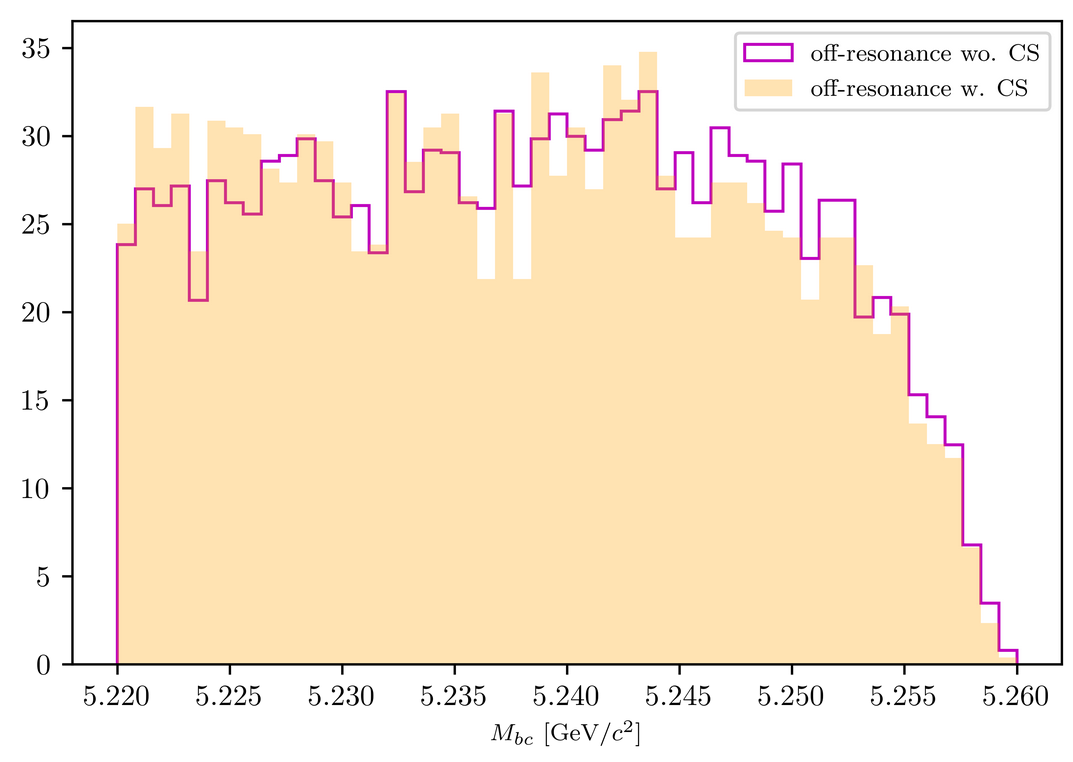
\includegraphics[width=.65\textwidth]{04-SimultaneousFit/figs/corrLambdaC_OffResonance_w_wo_CS_comparison_Data.png}} 
\caption{Above: $M_{bc}$ distributions of the MC off-resonance sample (5 streams) with and without continuum suppression. Below: $M_{bc}$ distributions on data with and without continuum suppression.}
\end{figure}




\noindent The validity of the method relies on the fact that the difference between  on-/off-resonance continuum events are well modeled in MC and that the shape of the $M_{bc}$ distribution doesn't change significantly when removing the continuum suppression cut both on MC and data (as one can see from Figures \ref{fig:corrLambdaC_OffResonance_w_wo_CS_comparison_5streams} - \ref{fig:corrLambdaC_OffResonance_w_wo_CS_comparison_Data}).\\
Additionally, the continuum suppression cut efficiency should be the same in data and MC in order to have the correct scaling on data with the above mentioned method. Fig. \ref{fig:R2_MC-Data_off_resonance_distributions} shows the distribution of the $foxWolframR2$ variable in off-resonance MC and data. The slight shift visible in data can cause a different impact on data in terms of rejected continuum background when applying the $foxWolframR2 < 0.3$ cut. It is found to reject about 60$\%$ of the continuum background in data, whereas it rejects 55$\%$ of the continuum background in MC ( 56$\%$ in on-resonance MC). Therefore in data one can expect about 2.25$\%$ less continuum background events. This discrepancy is not statistically significant (the statistical uncertainty for the continuum background events is of the level of $\sim 1\%$),  a simple correction to the number of events can be applied on data and its possible systematics can be then taken into account.



\begin{figure}
\centering
{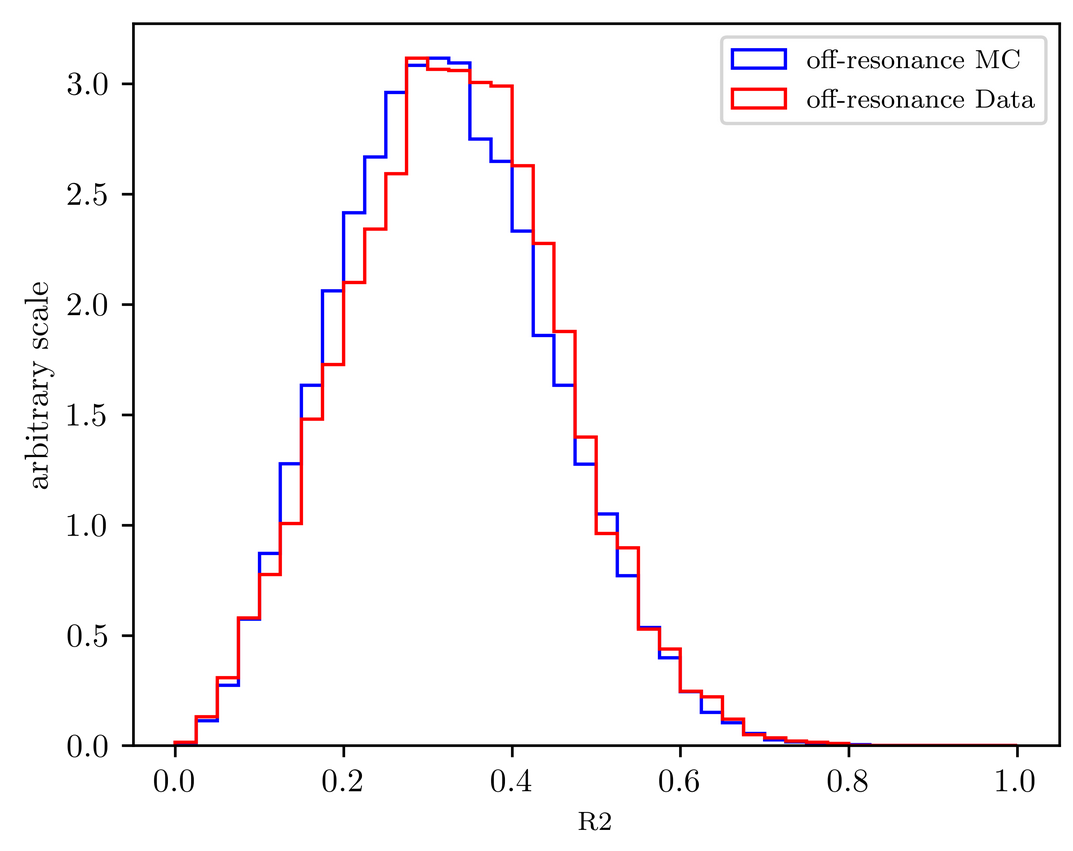
\includegraphics[width=0.5\textwidth]{04-SimultaneousFit/figs/R2_MC-Data_off_resonance_distributions.png}}
\caption{Distributions of variable $foxWolframR2$ in off-resonance MC and data.}
\label{fig:R2_MC-Data_off_resonance_distributions}
\end{figure}

\noindent  The obtained distribution can be then fitted with a Novosibirsk function (see Fig. \ref{fig:charged_corrLambdaC_Mbc_continuumMC_fit}). \\
This is the procedure which can be then applied on the off-resonance data to obtain the $M_{bc}$ shape describing the continuum background in data.
\begin{figure}
\centering
{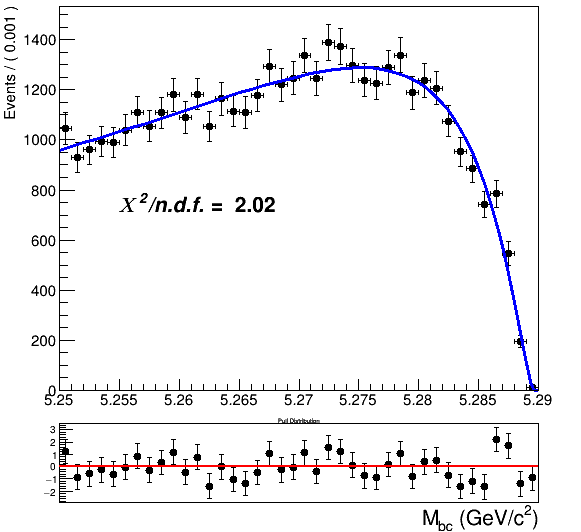
\includegraphics[width=0.43\textwidth]{04-SimultaneousFit/figs/stream5_rescaledMbc_40binsHist.png}}
\caption{Fit of the $M_{bc}$ distribution   MC (scaled) off-resonance continuum (one stream).}
\label{fig:charged_corrLambdaC_Mbc_continuumMC_fit}
\end{figure}

In the $\Lambda_c$ invariant mass one doesn't expect correlation effects, but nevertheless there can be differences due to the limited statistics of the off-resonance sample. 
In fact, in the case of on-resonance MC for the charged correlated decays some events in which  $\Lambda_c$ candidates survive nominal selection cuts are visible and can be described with a small Gaussian on the top of the flat background (Fig.\ref{fig:onRes_InvM_corrLambdaC}). Due to the low statistics one cannot see a similar peak in the off-resonance sample (the Fig.\ref{fig:5streams_offRes_InvM_corrLambdaC} shows a 5 streams statistics).

The shape describing the $\Lambda_c$ invariant mass in the case of charged correlated decays is obtained from the simulated on-resonance continuum, again using 5 streams statistics (see Fig. \ref{fig:onRes_InvM_corrLambdaC} ). In the other cases no peak is visible and therefore also the $\Lambda_c$ invariant mass shape is obtained from 5 streams of off-resonance events.


\begin{figure}
\centering
\subcaptionbox{\label{fig:onRes_InvM_corrLambdaC}}
{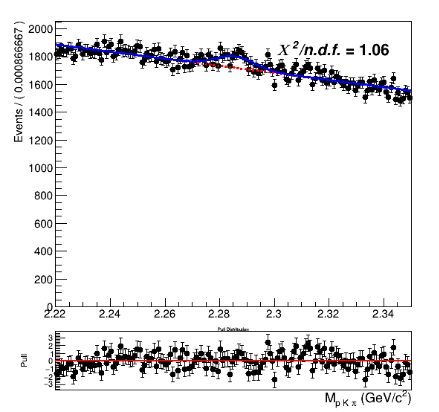
\includegraphics[width=.45\textwidth]{04-SimultaneousFit/figs/onRes_InvM_corrLambdaC.png}} 
\subcaptionbox{\label{fig:5streams_offRes_InvM_corrLambdaC}}
{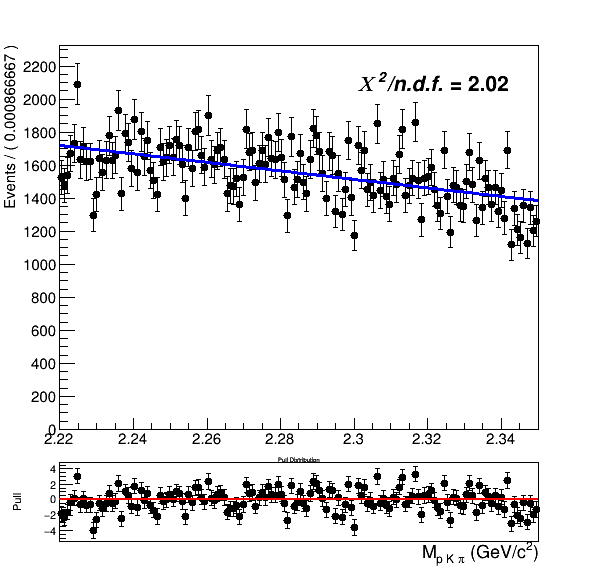
\includegraphics[width=.46\textwidth]{04-SimultaneousFit/figs/5streams_Off_resonanceRescaledContinuum_charged_corrLambdaC_oneGaussianInvMfit.png}} 
\caption{Comparison between 5 streams of MC on-resonance continuum \ref{fig:onRes_InvM_corrLambdaC}) and off-resonance (scaled) continuum in $M(p K \pi)$ (\ref{fig:5streams_offRes_InvM_corrLambdaC}).}
%\label{}
\end{figure}
%\newpage

Finally, it is possible to examine the validity of the whole procedure on the independent stream. 
Fig. \ref{fig:stream3corrLambddaC_total_continuum_2DFit} - \ref{fig:stream0_neutral_anticorrLambddaC_total_continuum_2DFit} show the $M_{bc}$, $M(p K \pi)$ projections of the overlayed two dimensional PDFs  obtained with the above described procedure.\\
The 2D PDF used for Fig. \ref{fig:stream3corrLambddaC_total_continuum_2DFit} can be written as: \\
 \vspace{0.2 cm}

$P^{Continuum}_{B,\Lambda_c}(M_{bc}, M(p K \pi)) = \Gamma_{Nov}(M_{bc}) \times [\rho_{Cheb1}(M(p K \pi) + \rho_{G}(M(p K \pi))]$\\
\vspace{0.2 cm}

where, as already anticipated, the invariant mass is described by a sum of a first order Chebychev polynomial and the peak by the same triple Gaussian PDF adopted for the signal. The  2D PDF used for Fig. \ref{fig:stream0_anticorrLambddaC_total_continuum_2DFit_Novosibirsk} and Fig. \ref{fig:stream0_neutral_corrLambddaC_total_continuum_2DFit_Novosibirsk} differ only in the invariant mass, not having the triple gaussian. Whereas the 2D PDF used for Fig. \ref{fig:stream0_neutral_anticorrLambddaC_total_continuum_2DFit} can be written as: \\
 \vspace{0.2 cm}

$P^{Continuum}_{B,\Lambda_c}(M_{bc}, M(p K \pi)) = \Gamma_{Argus}(M_{bc}) \times [\rho_{Cheb1}(M(p K \pi) ]$\\
\vspace{0.2 cm}

since the distribution in $M_{bc}$ can be better described by an Argus.
\begin{figure}
%\centering
{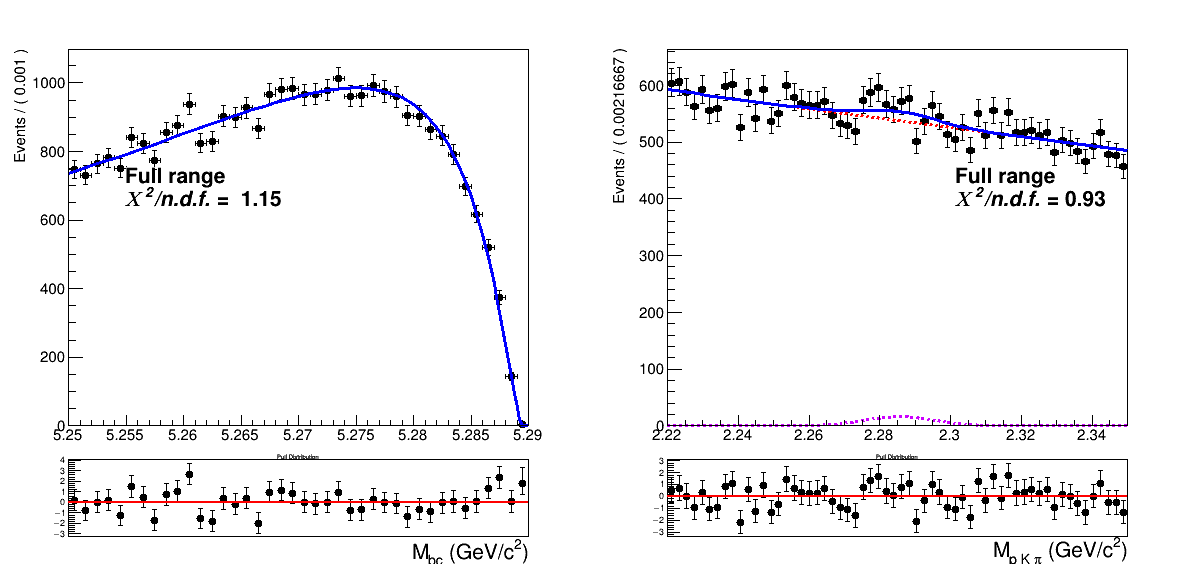
\includegraphics[width=0.85\textwidth]{04-SimultaneousFit/figs/stream3corrLambddaC_total_continuum_2DFit.png}}
\caption{Two dimensional fit of charged correlated  continuum events (one stream).}
\label{fig:stream3corrLambddaC_total_continuum_2DFit}
\end{figure}


\begin{figure}
%\centering
{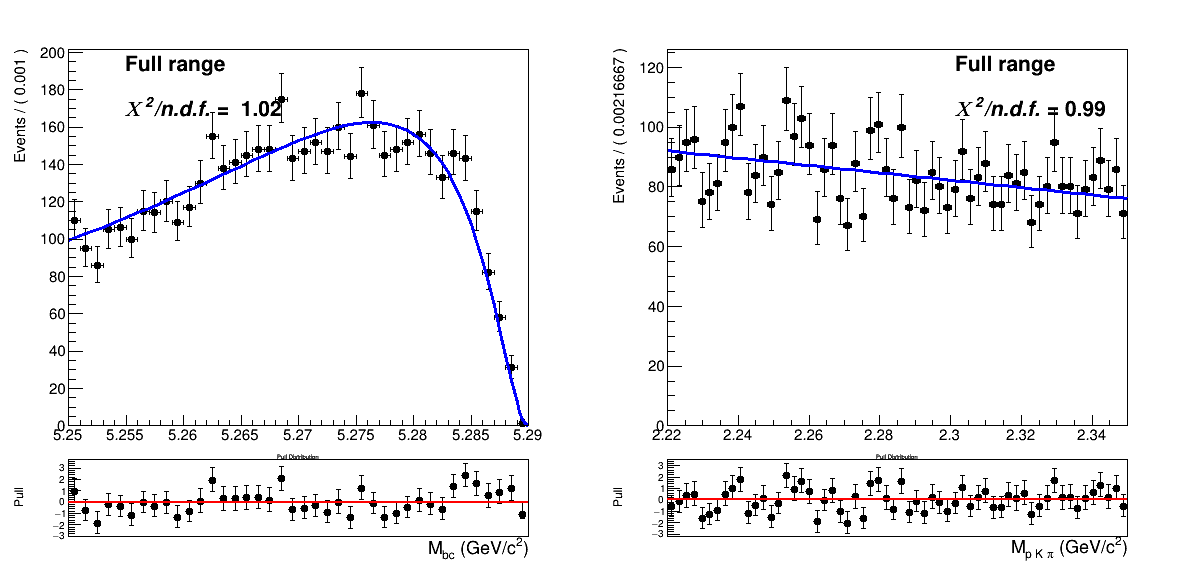
\includegraphics[width=0.85\textwidth]{04-SimultaneousFit/figs/stream0_anticorrLambddaC_total_continuum_2DFit_Novosibirsk.png}}
\caption{Two dimensional fit of charged anticorrelated continuum events (one stream).}
\label{fig:stream0_anticorrLambddaC_total_continuum_2DFit_Novosibirsk}
\end{figure}

\begin{figure}
%\centering
{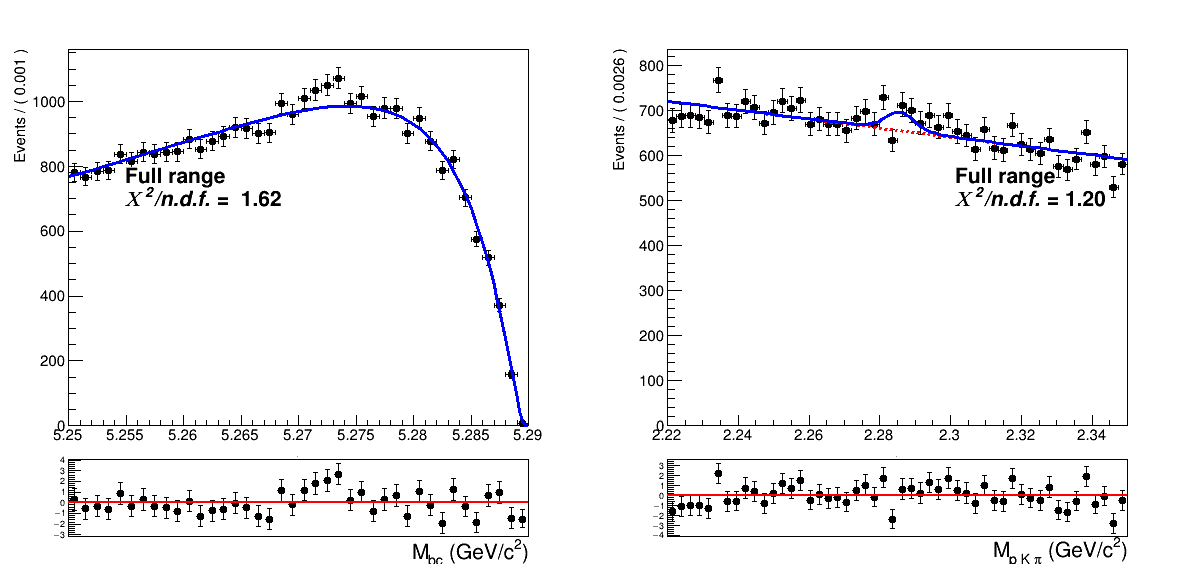
\includegraphics[width=0.85\textwidth]{04-SimultaneousFit/figs/stream0corrLambddaC_total_continuum_2DFit.png}}
\caption{Two dimensional fit of  continuum events (one stream).}
\label{fig:stream0_neutral_corrLambddaC_total_continuum_2DFit_Novosibirsk}
\end{figure}

\begin{figure}
%\centering
{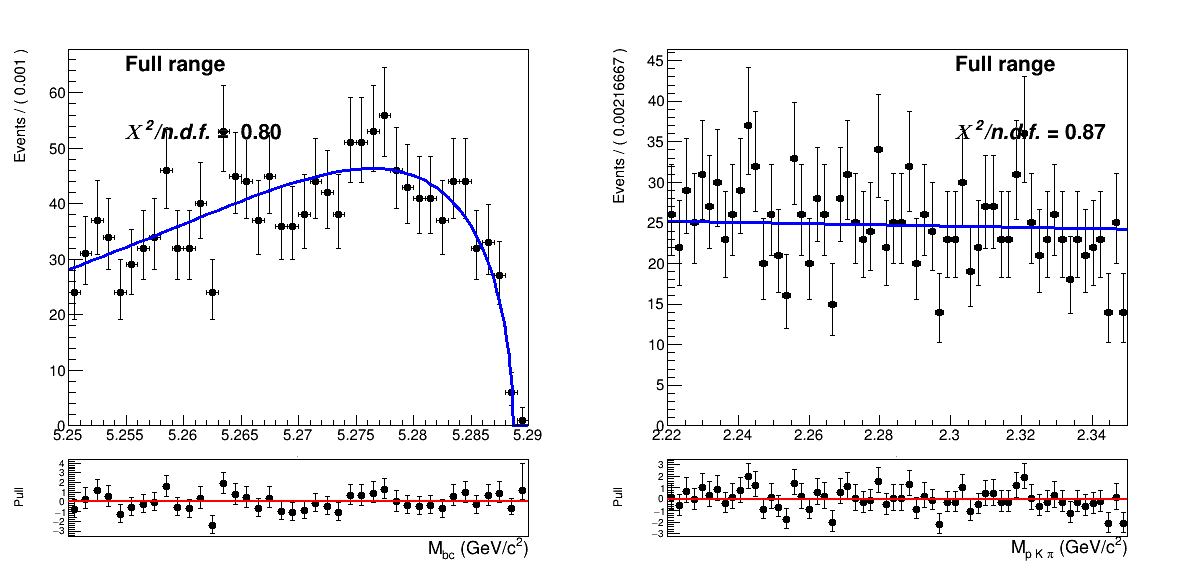
\includegraphics[width=0.85\textwidth]{04-SimultaneousFit/figs/stream0_anticorrLambddaC_total_continuum_2DFit_Argus.png}}
\caption{Two dimensional fit of  continuum events (one stream).}
\label{fig:stream0_neutral_anticorrLambddaC_total_continuum_2DFit}
\end{figure}


\newpage

\section{Two dimensional fit on Monte Carlo}\label{MC2D_Fit}

A total of six independent streams were used to construct/validate the fit model: each time five streams were 
used to construct the already discussed PDFs and the independent stream is used to test if the total PDF enables to extract 
the signal yield in an unbiased way (a total of six fits are performed on the six different streams of generic MC).\\
To especially suppress the systematic uncertainties deriving from the amount of crossfeed the samples corresponding to the four
different decay channels are fitted simultaneously.
In all six fits all the shaping parameters are kept fixed, except:
\begin{itemize}
    \item $\sigma_{G1}$: the width of the main of the three Gaussian functions in $\rho_G(M(p K \pi))$
    \item $\sigma_{CB}$ parameter for the Crystal Ball describing the signal peak in $M_{bc}$
\end{itemize}

\noindent In the $M_{bc}$ distribution the $\sigma_{CB}$ width parameter for the Crystal Ball describing the $M_{bc}$ peaking background is expressed as function of the signal $\sigma_{CB}$  with a ratio fixed from MC.

\noindent As for the normalizations, mis-/reconstructed signal events  and  $M_{bc}$ peaking/flat background events are floated in the two dimensional unbinned maximum likelihood fits. 
The continuum background normalization is kept fixed to the value obtained by the off-resonance scaling procedure. \\
Instead, the normalization of crossfeed background events is determined by the fit in the following way:

\begin{equation}
N_{CrossBkg} =  N_{recSig}^{corr} \cdot (\epsilon_{cross}/\epsilon_{recSig})^{corr} + N_{recSig}^{anticorr} \cdot (\epsilon_{cross}/\epsilon_{recSig})^{anticorr}  
\label{eq:paramCrossfeedNorm}
\end{equation}

where $N_{recSig}^{corr}$ ($N_{recSig}^{anticorr}$) are the fitted signal yields of the corresponding crossfeeding decay and $ (\epsilon_{cross}/\epsilon_{recSig})$ are the ratios of misreconstruction efficiency and signal reconstruction efficiency as determined in the Monte Carlo.
Since the crossfeed can likely occur both from correlated and anticorrelated channels, both are considered and summed together.\\
Exemplary, the distributions of stream 0 overlaid by the fitted PDF are depicted in \crefrange{fig:charged_corrSample_simultaneous2DFit_stream0}{fig:neutral_anticorrSample_simultaneous2DFit_stream0}.
In Tables \ref{tab:SixStreams_chargedCorrLam2Dfits} to \ref{tab:SixStreams_neutral_anticorrLam2Dfits}  the signal yields of the fits (\textbf{Reconstructed Signal}) to the two dimensional distributions for the six streams are listed and compared
to the yields obtained from fits of signal distributions of each individual stream. The latter are the "expected" yields of reconstructed signal from a fit to the total signal events in the individual
stream as the one plotted on \cref{fig:stream0_TotalSignal_charged_corrLambdaC_2Dfit} where all the parameters of the PDFs described in \cref{eq:RecSigEq} are kept fixed and the corresponding yields are extracted from the fit. 
Note that in the case of Tables \cref{tab:SixStreams_neutralCorrLam2Dfits} - \ref{tab:SixStreams_neutral_anticorrLam2Dfits}  the reconstructed signal yields are contaminated by events from the other neutral $B^0$ decay channel
 that experience mixing. Since those events cannot be analytically distinguished from the true signal events, the branching fraction calculation for neutral decays needs to take them into account and correct for their contribution 
 (as will be shown in the next Chapter).


 \begin{figure}[H]
    %\centering
    {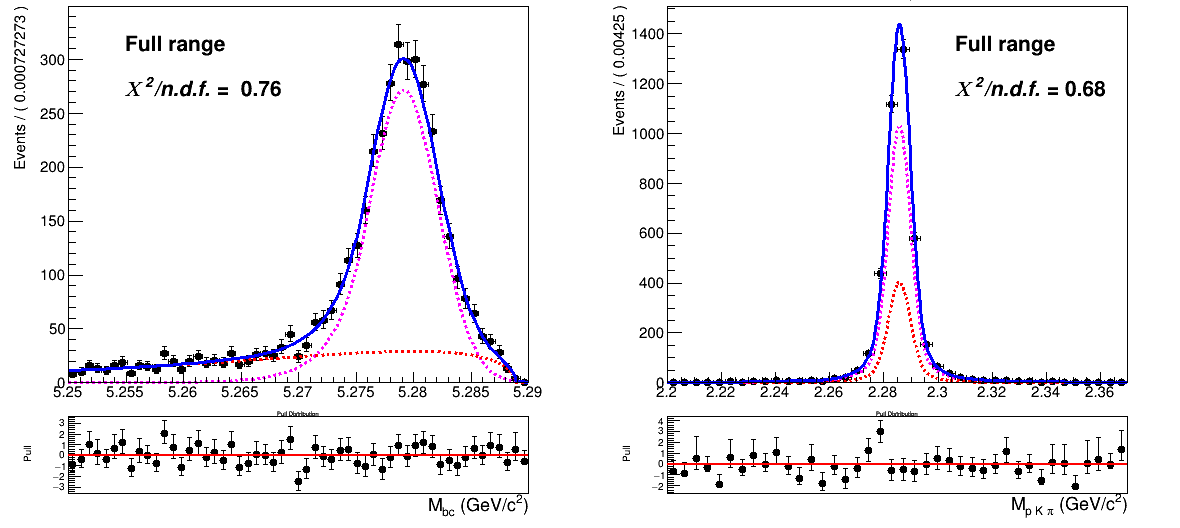
\includegraphics[width=0.75\textwidth]{04-SimultaneousFit/figs/stream0_TotalSignal_charged_corrLambdaC_2Dfit.png}}
    \caption{Two dimensional fit of Total Signal of stream 0 used to extract the expected reconstructed (corresponding to the PDF colored in magenta) and expected misreconstructed yields (corresponding to the PDF colored in red).}
    \label{fig:stream0_TotalSignal_charged_corrLambdaC_2Dfit}
    \end{figure}


\newpage

\subsection{Fit results for $B^- \rightarrow \Lambda_c^+$ decays}  

\begin{figure}[H]
\centering
{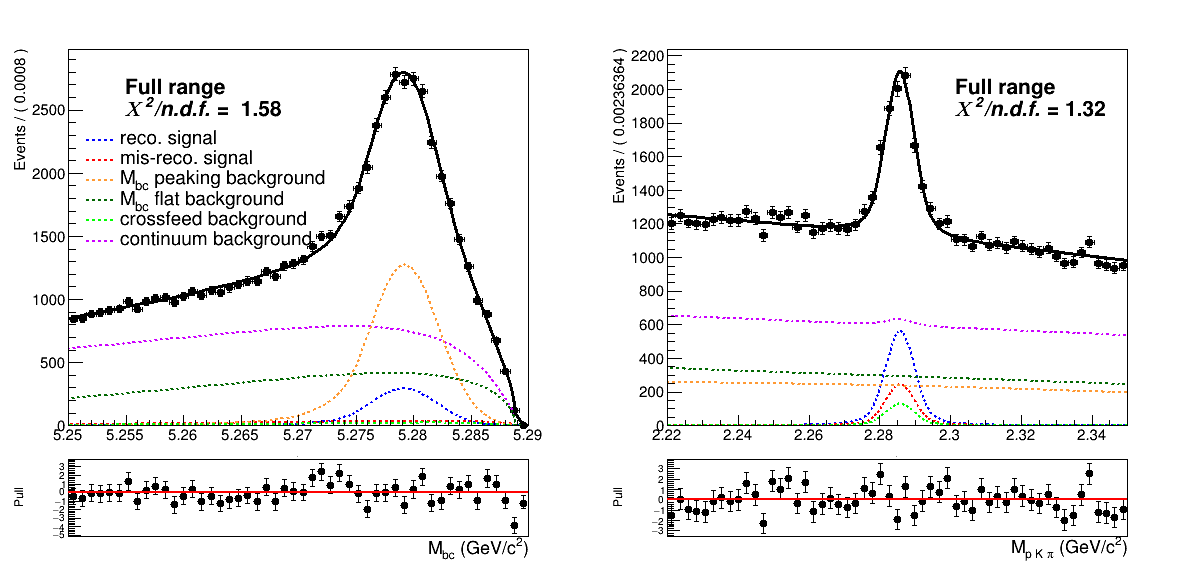
\includegraphics[width=0.90\textwidth]{04-SimultaneousFit/figs/charged_corrSample_simultaneous2DFit_stream0.png}}
\caption{Projections of the two dimensional simultaneous fit on stream 0 Monte Carlo simulated data for charged correlated decays.}
\label{fig:charged_corrSample_simultaneous2DFit_stream0}
\end{figure}

\begin{figure}[H]
    \centering
    
    {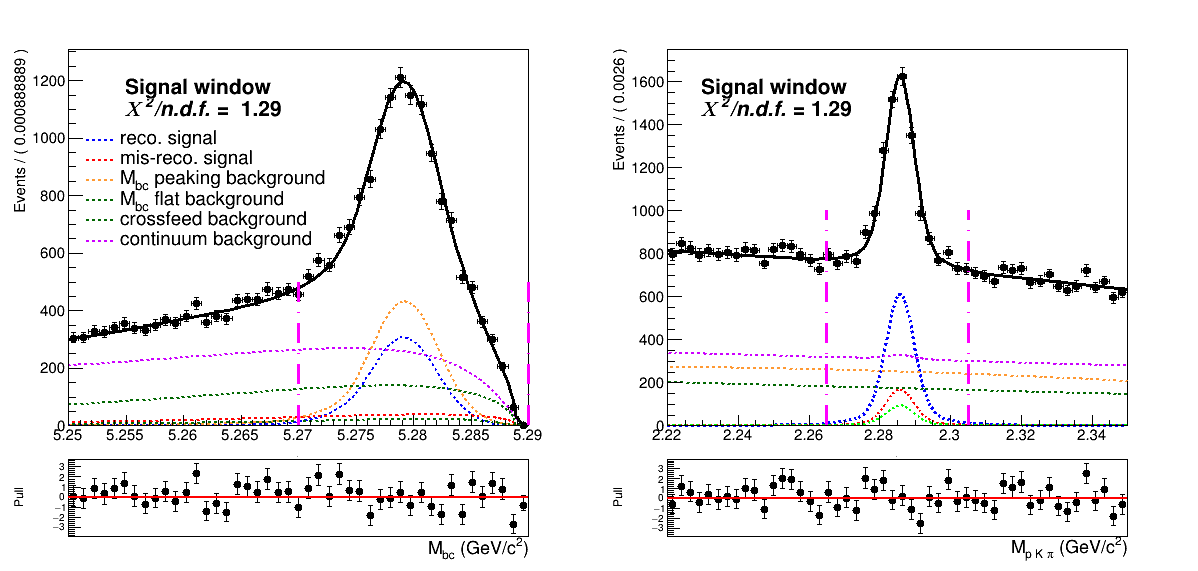
\includegraphics[width=0.90\textwidth]{04-SimultaneousFit/figs/charged_corrSignal_window_Total_2DFit_stream0.png}}
    \caption{Projections of the two dimensional simultaneous fit on stream 0 Monte Carlo simulated data for charged correlated decays(in the signal window) }
    \label{fig:charged_corrSignal_window_Total_2DFit_stream0}
    \end{figure}

\begin{table}[H]
    \centering
    \resizebox{0.99\textwidth}{!}{%
    \setlength{\tabcolsep}{8pt}
    \begin{tabular}{c c c c c c c}
    
    \toprule
     \hline
       &	\multicolumn{2}{c}{Reconstructed Signal}  & \multicolumn{2}{c}{Total Signal} &  \\
         &  fit \hspace{0.5 cm}  & expected  & fit   & MC truth &  \multicolumn{2}{c}{fit - MC truth} \\
     \midrule
     \hline
    stream 0	&	2829 $\pm$ 130 	&	2928 $\pm$ 66	&	4063 $\pm$ 157	&	4061	&  -2	&	-0.05$\%$	\\
    stream 1	&	2811 $\pm$ 137	&	2956 $\pm$ 65	&	4095 $\pm$ 161	&	4084	&  11	&	0.3$\%$	\\
    stream 2	&	2952 $\pm$ 141	&	2940 $\pm$ 65	&	4345 $\pm$ 165	&	4138	& 207	&	5.0$\%$	\\
    stream 3	&	2747 $\pm$ 134	&	2867 $\pm$ 66	&	4267 $\pm$ 160	&	4105	& 162  &   	3.9$\%$	\\
    stream 4	&	3043 $\pm$ 138	&	3017 $\pm$ 67	&	4148 $\pm$ 157	&	4176	& -28	&	-0.7$\%$	\\
    stream 5	&	2818 $\pm$ 136	&	2816 $\pm$ 65	&	3999 $\pm$ 162	&	4001	&  -2	&	-0.05$\%$	\\
    \midrule
    \hline
    sum			&	17200		&	17524	&		24917		&	24565	&	348	&	1.4$\%$	\\
    \bottomrule
    \hline
    \end{tabular}%
    }%
    \caption{Charged correlated decays: comparison of fitted and expected signal yields, fitted and truth-matched total signal for six streams of Belle generic MC when fitting the two dimensional distributions of $M_{bc}$ and $M(p K \pi)$.}
    \label{tab:SixStreams_chargedCorrLam2Dfits}
    \end{table}
    

    The yields obtained by the fit show a slight tendency of underestimation, but when comparing the sums of them with the sum of expected 
    values one can see the difference is within statistical fluctuations ( within 2$\%$). 
   \\
   The tendency of underestimation is visible in , but it is just slightly larger than $\sigma$


   \begin{figure}[H]
    \centering
    {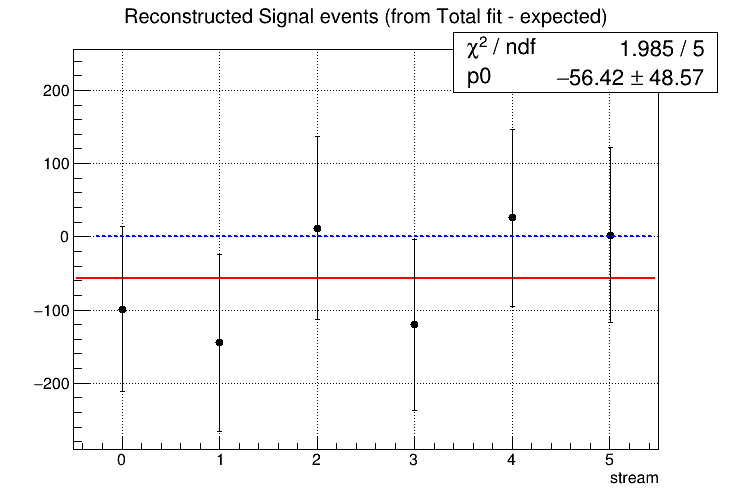
\includegraphics[width=0.70\textwidth]{04-SimultaneousFit/figs/6streamResults_chargedCorrelated_correct.png}}
    \caption{Residuals of signal yields (alias reconstructed signal, values reported in the first two columns of the above displayed table).}
    \label{fig:6streamsResults_chargedCorrelated}
    \end{figure}


\newpage    

\subsection{Fit results for $B^- \rightarrow \bar{\Lambda}_c^-$ decays}   

For the anticorrelated decays from charged $B$ mesons the slight tendency is in the opposite direction. But the distribution of residuals (see \cref{fig:6streamsResults_chargedAnticorrelated})
shows this slight overestimation is well within the statistical uncertainty.



\begin{table}[b]
    \centering
    \resizebox{0.95\textwidth}{!}{%
    \setlength{\tabcolsep}{8pt}
    \begin{tabular}{c c c c c c c}
    
    \toprule
     \hline
       &	\multicolumn{2}{c}{Reconstructed Signal}  & \multicolumn{2}{c}{Total Signal} &  \\
         &  fit \hspace{0.5 cm}  & expected  & fit   & MC truth &  \multicolumn{2}{c}{fit - MC truth} \\
     \midrule
     \hline
    stream 0	&	724 $\pm$ 64 	&	695 $\pm$ 28	&	813 $\pm$ 73	&	765	&  48	&	6.3$\%$	\\
    stream 1	&	726 $\pm$ 65	&	709 $\pm$ 29	&	802 $\pm$ 67	&	785	&  17	&	2.2$\%$	\\
    stream 2	&	788 $\pm$ 72	&	718 $\pm$ 29	&	911 $\pm$ 72	&	797	& 114	&	14.3$\%$	\\
    stream 3	&	679 $\pm$ 60	&	702 $\pm$ 29	&	768 $\pm$ 66	&	802	& -34  &   	4.2$\%$	\\
    stream 4	&	844 $\pm$ 73	&	710 $\pm$ 29	&	982 $\pm$ 73	&	785	& 197	&	25.1$\%$	\\
    stream 5	&	605 $\pm$ 63	&	675 $\pm$ 29	&	722 $\pm$ 63	&	760	&  -38	&	-5.0$\%$	\\
    \midrule
    \hline
    sum			&	4366		&	4209	&		4998		&	4694	&	304	&	6.5$\%$	\\
    \bottomrule
    \hline
    \end{tabular}%
    }%
    \caption{Charged anticorrelated decays: comparison of fitted and expected signal yields, fitted and truth-matched total signal for six streams of Belle generic MC when fitting the two dimensional distributions of $M_{bc}$ and $M(p K \pi)$.}
    \label{tab:SixStreams_chargedAntiLam2Dfits}
    \end{table}

    \begin{figure}[H]
        \centering
        {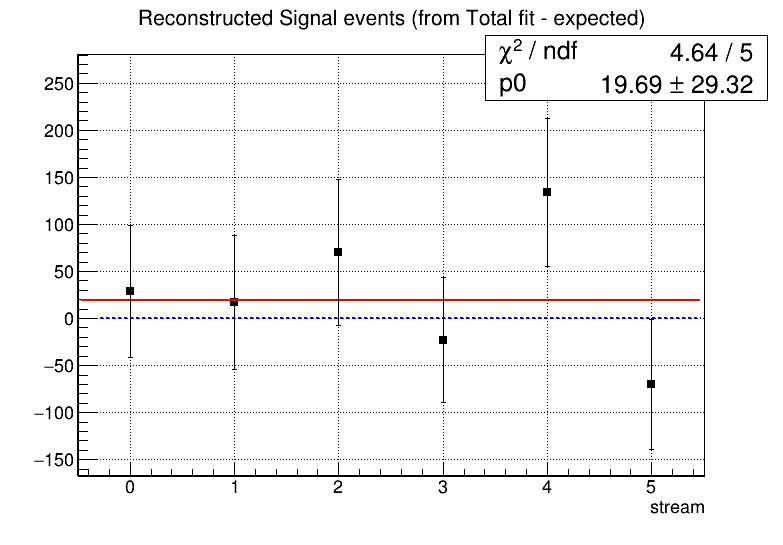
\includegraphics[width=0.70\textwidth]{04-SimultaneousFit/figs/6streamsResults_chargedAnticorrelated.png}}
        \caption{Residuals of signal yields (alias reconstructed signal, values reported in the first two columns of the above displayed table).}
        \label{fig:6streamsResults_chargedAnticorrelated}
        \end{figure}

\begin{figure}[H]
\centering
{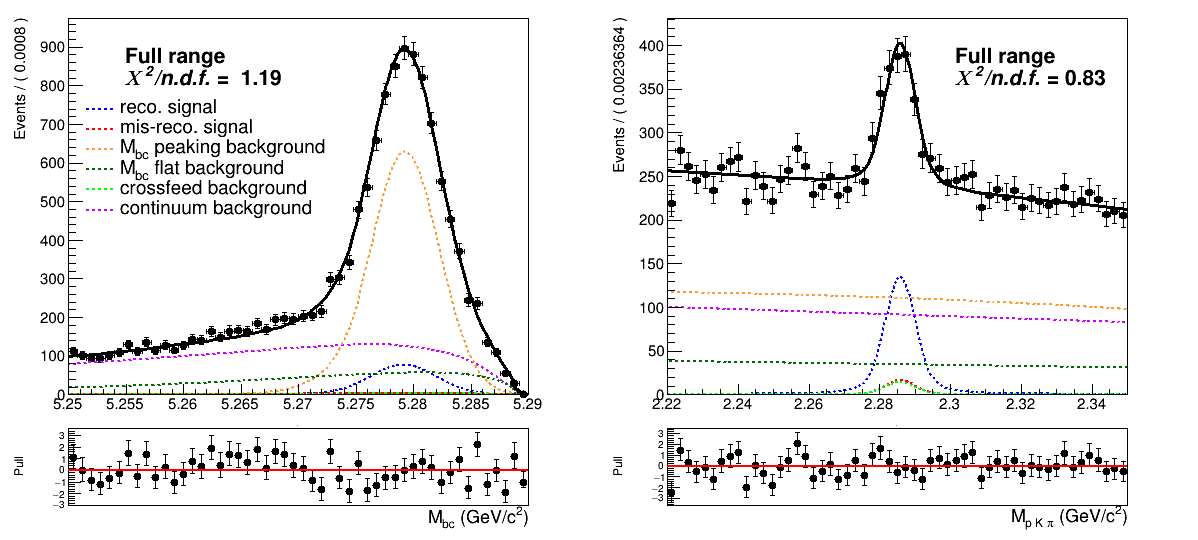
\includegraphics[width=0.90\textwidth]{04-SimultaneousFit/figs/charged_antiSample_simultaneous2DFit_stream0.png}}
\caption{Projections of the two dimensional simultaneous fit on stream 0 Monte Carlo simulated data for charged anticorrelated decays.}
\label{fig:charged_antiSample_simultaneous2DFit_stream0}
\end{figure}

\begin{figure}[H]
    \centering
    {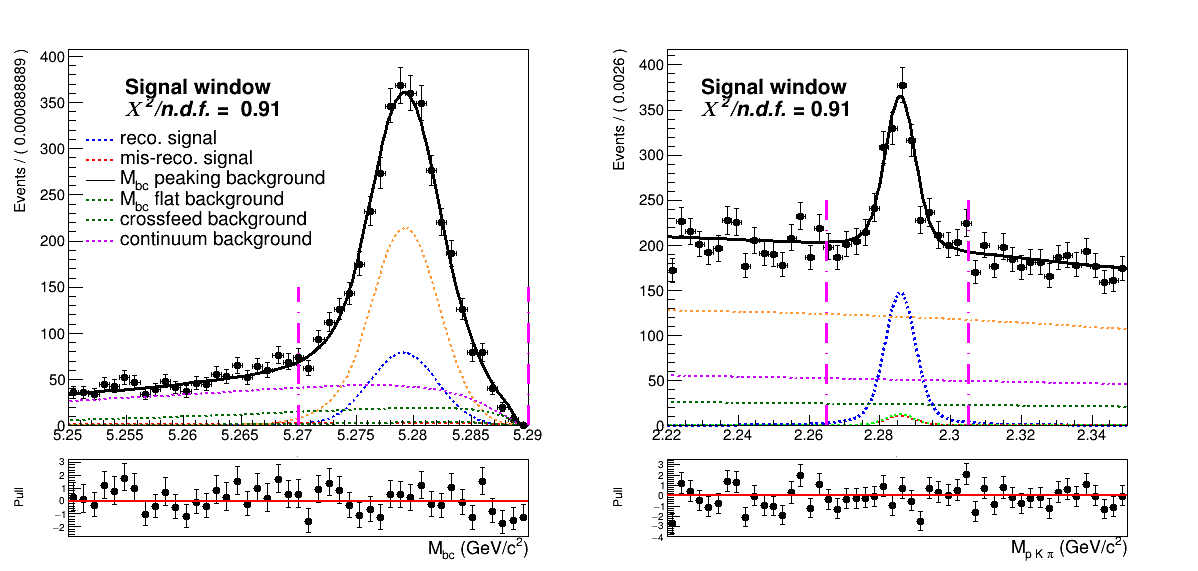
\includegraphics[width=0.90\textwidth]{04-SimultaneousFit/figs/charged_antiSignal_window_Total_2DFit_stream0.png}}
    \caption{Projections of the two dimensional simultaneous fit on stream 0 Monte Carlo simulated data for charged anticorrelated decays (in the signal window).}
    \label{fig:charged_antiSignal_window_Total_2DFit_stream0}
    \end{figure}

\newpage
\subsection{Fit results for $\bar{B^0} \rightarrow \Lambda_c^+$ decays}  
    
Also in the case of the neutral correlated one can observe a slight overestimation in the reconstructed signal yields.
The residuals (see \cref{fig:RecoSignal_streams_fit_neutralCorrLambdaC}) show that this is not so negligible: 
the significance is about 1.5$\sigma$.

\begin{table}[H]
    \centering
    \resizebox{0.95\textwidth}{!}{%
    \setlength{\tabcolsep}{8pt}
    \begin{tabular}{c c c c c c c}
    
    \toprule
     \hline
       &	\multicolumn{2}{c}{Reconstructed Signal}  & \multicolumn{2}{c}{Total Signal} &  \\
         &  fit \hspace{0.5 cm}  & expected  & fit   & MC truth &  \multicolumn{2}{c}{fit - MC truth} \\
     \midrule
     \hline
    stream 0	&	1329 $\pm$ 69 	&	1240 $\pm$ 38	&	1390 $\pm$ 70	&	1379	&  11	&	0.8$\%$	\\
    stream 1	&	1314 $\pm$ 68	&	1327 $\pm$ 38	&	1319 $\pm$ 66	&	1287	&  14	&	2.5$\%$	\\
    stream 2	&	1266 $\pm$ 68	&	1254 $\pm$ 38	&	1273 $\pm$ 65	&	1251	& 22	&	1.8$\%$	\\
    stream 3	&	1320 $\pm$ 67	&	1248 $\pm$ 38	&	1316 $\pm$ 66	&	1255	& 35  &   	4.9$\%$	\\
    stream 4	&	1227 $\pm$ 67	&	1214 $\pm$ 38	&	1300 $\pm$ 66	&	1223	&  77	&	6.3$\%$	\\
    stream 5	&	1282 $\pm$ 70	&	1233 $\pm$ 38	&	1251 $\pm$ 66	&	1246	&  5	&	0.4$\%$	\\
    \midrule
    \hline
    sum			&	7738		&	7516	&		7709		&	7525	&	140	&	1.86$\%$	\\
    \bottomrule
    \hline
    \end{tabular}%
    }%
    \caption{Comparison of fitted and expected signal yields, fitted and truth-matched total signal for six streams of Belle generic MC when fitting the two dimensional distributions of $M_{bc}$ and $M(p K \pi)$.}
    \label{tab:SixStreams_neutralCorrLam2Dfits}
    \end{table}
    
    

\begin{figure}[H]
\centering
{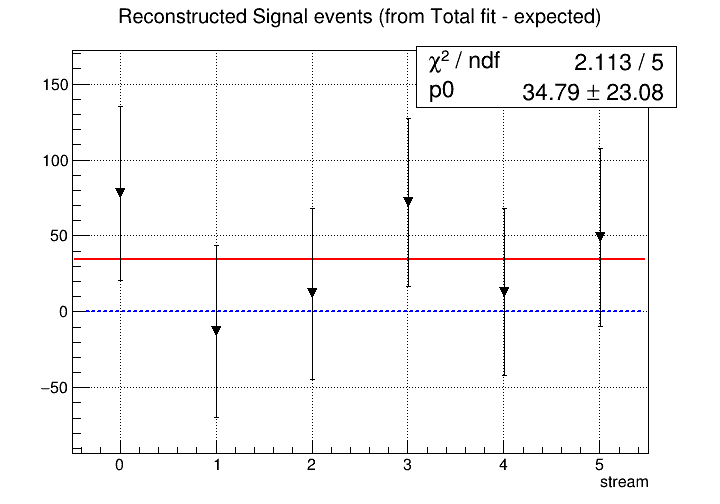
\includegraphics[width=0.70\textwidth]{04-SimultaneousFit/figs/RecoSignal_streams_fit_neutralCorrLambdaC.png}}

\caption{Residuals of signal yields for neutral correlated decays.}
        \label{fig:RecoSignal_streams_fit_neutralCorrLambdaC}
        \end{figure}    

\begin{figure}[H]
\centering
{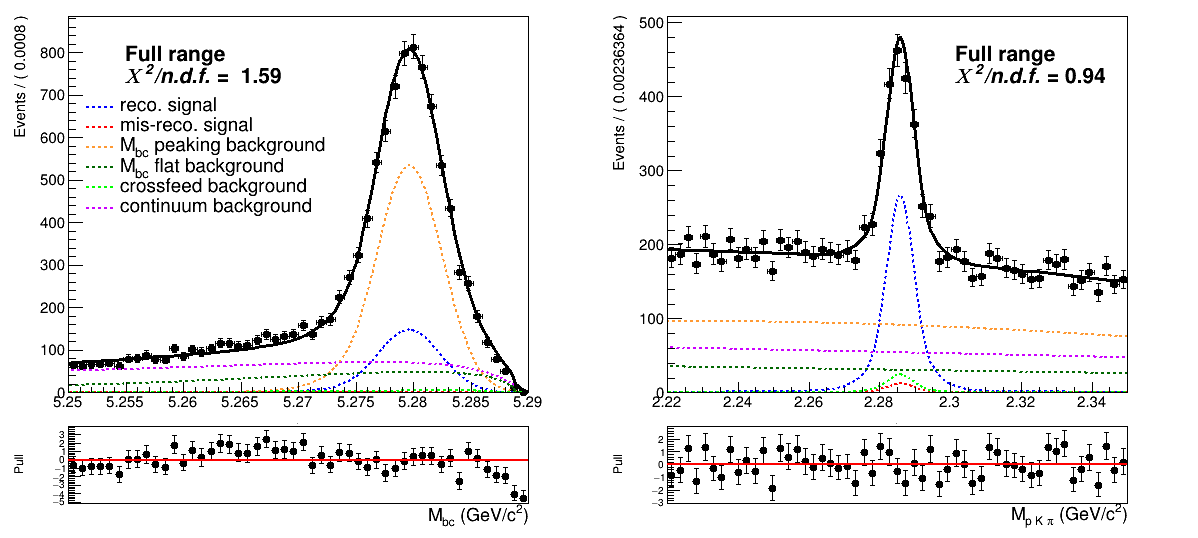
\includegraphics[width=0.90\textwidth]{04-SimultaneousFit/figs/neutral_corrSample_simultaneous2DFit_stream0.png}}
\caption{Projections of the two dimensional simultaneous fit on stream 0 Monte Carlo simulated data for neutral correlated decays.}
\label{fig:neutral_corrSample_simultaneous2DFit_stream0}
\end{figure}

\begin{figure}[H]
    \centering
    {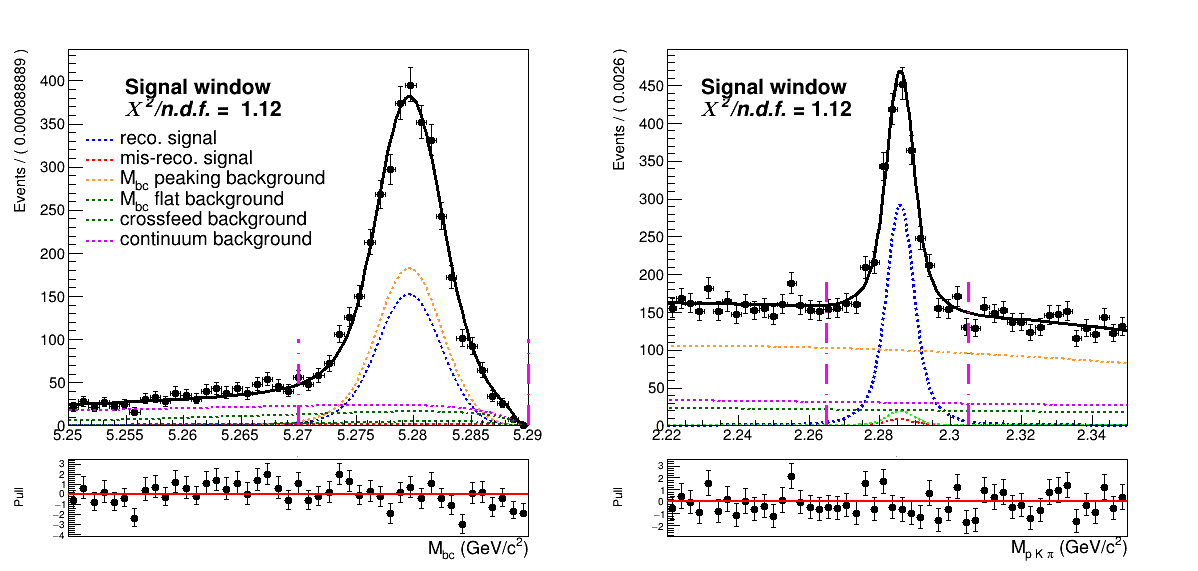
\includegraphics[width=0.90\textwidth]{04-SimultaneousFit/figs/neutral_corrSignal_window_Total_2DFit_stream0.png}}
    \caption{Projections of the two dimensional simultaneous fit on stream 0 Monte Carlo simulated data for neutral correlated decays.}
    \label{fig:neutral_corrSignal_window_Total_2DFit_stream0}
    \end{figure}



    
    \begin{figure}[H]
        \centering
        {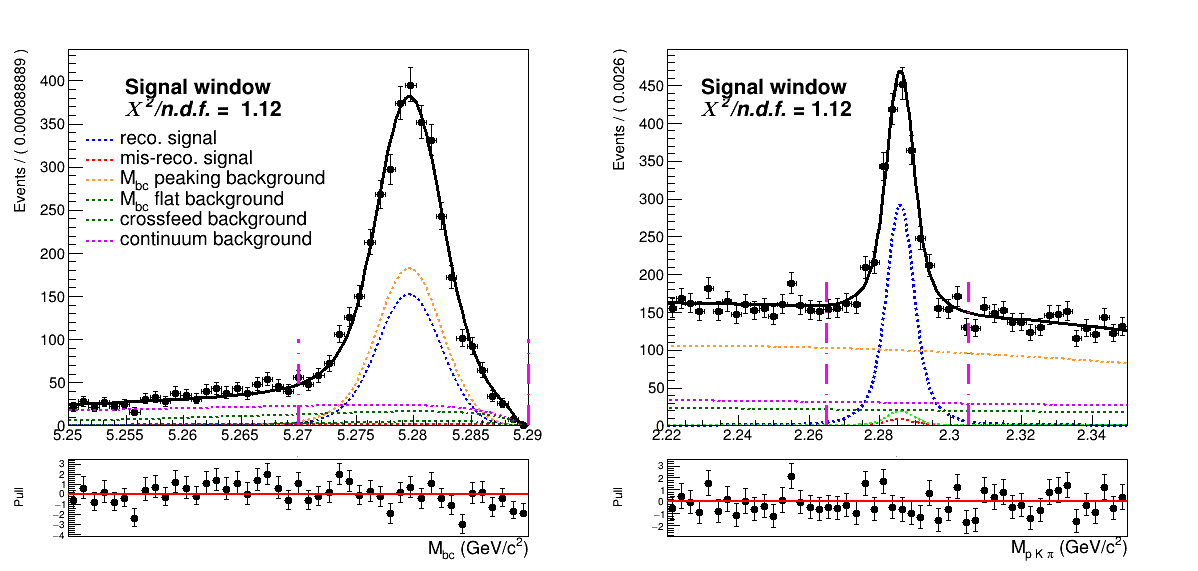
\includegraphics[width=0.90\textwidth]{04-SimultaneousFit/figs/neutral_corrSignal_window_Total_2DFit_stream0.png}}
        \caption{Projections of the two dimensional simultaneous fit on stream 0 Monte Carlo simulated data for neutral correlated decays (in the signal window).}
        \label{fig:neutral_corrSignal_window_Total_2DFit_stream0}
        \end{figure}

        
\subsection{Fit results for $\bar{B^0} \rightarrow \bar{\Lambda}_c^-$ decays} 


\begin{table}[H]
    \centering
    \resizebox{0.8\textwidth}{!}{%
    \setlength{\tabcolsep}{8pt}
    \begin{tabular}{c c c c c c c}
    
    \toprule
     \hline
       &	\multicolumn{2}{c}{Reconstructed Signal}  & \multicolumn{2}{c}{Total Signal} &  \\
         &  fit \hspace{0.5 cm}  & expected  & fit   & MC truth &  \multicolumn{2}{c}{fit - MC truth} \\
     \midrule
     \hline
    stream 0	&	567 $\pm$ 45 	&	575 $\pm$ 29	&	657 $\pm$ 45	&	668	& -11 	&	-1.6$\%$	\\
    stream 1	&	565 $\pm$ 46	&	607 $\pm$ 21	&	660 $\pm$ 47	&	687	&  -27	&	-3.9$\%$	\\
    stream 2	&	574 $\pm$ 46	&	593 $\pm$ 20	&	659 $\pm$ 45	&	639	& 20 &	3.1$\%$	\\
    stream 3	&	714 $\pm$ 49	&	596 $\pm$ 21	&	792 $\pm$ 52	&	680	& 112  &   	16.4$\%$	\\
    stream 4	&	603 $\pm$ 50	&	594 $\pm$ 21	&	693 $\pm$ 50	&	638	& 55	&	8.6$\%$	\\
    stream 5	&	589 $\pm$ 63	&	595 $\pm$ 21	&	603 $\pm$ 44	&	624	&  -21	&	3.4$\%$	\\
    \midrule
    \hline
    sum			&	3612		&	3560	&		4064		&	3936	&	170	&	4.3$\%$	\\
    \bottomrule
    \hline
    \end{tabular}%
    }%
    \caption{Neutral anticorrelated decays: comparison of fitted and expected signal yields, fitted and truth-matched total signal for six streams of Belle generic MC when fitting the two dimensional distributions of $M_{bc}$ and $M(p K \pi)$.}
    \label{tab:SixStreams_neutral_anticorrLam2Dfits}
    \end{table}

\begin{figure}
\centering
{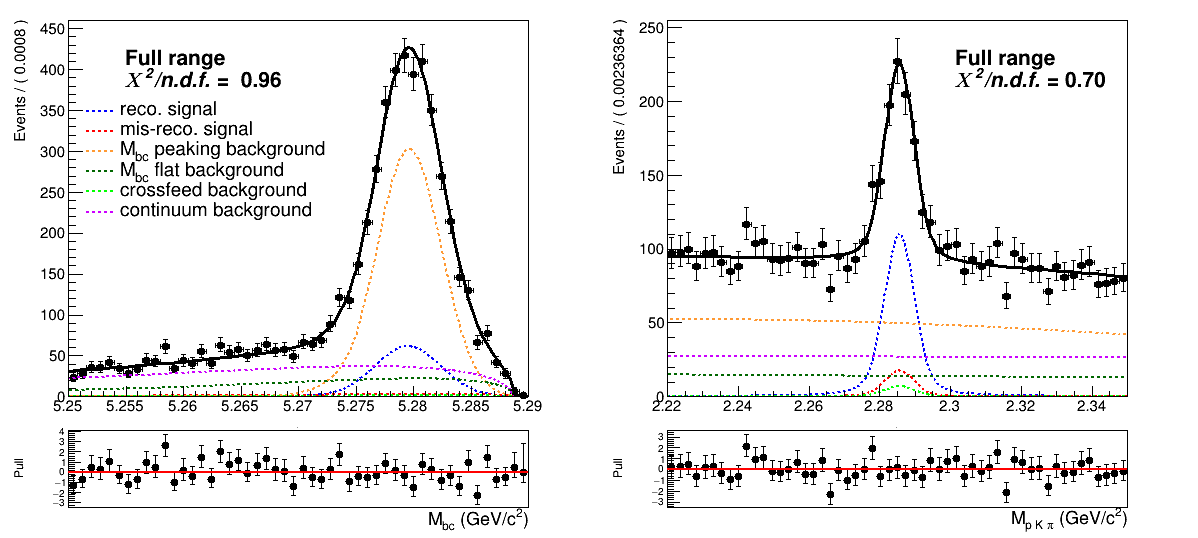
\includegraphics[width=0.83\textwidth]{04-SimultaneousFit/figs/neutral_anticorrSample_simultaneous2DFit_stream0.png}}
\caption{Projections of the two dimensional simultaneous fit on stream 0 Monte Carlo simulated data for neutral anticorrelated decays.}
\label{fig:neutral_anticorrSample_simultaneous2DFit_stream0}
\end{figure}

    \begin{figure}[H]
        \centering
        {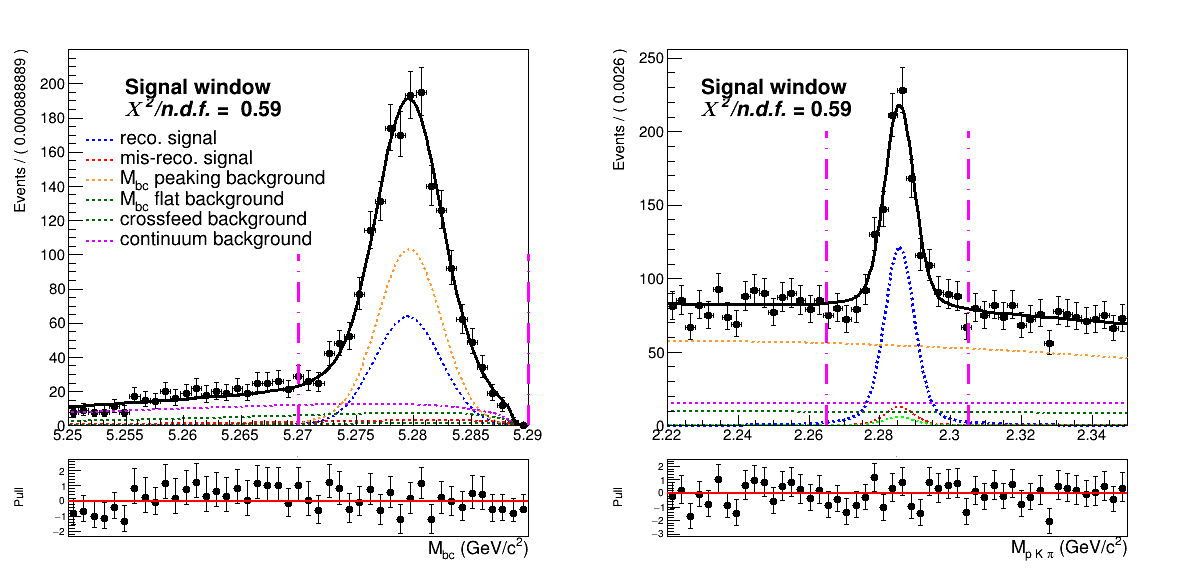
\includegraphics[width=0.90\textwidth]{04-SimultaneousFit/figs/neutral_antiSignal_window_Total_2DFit_stream0.png}}
        \caption{Projections of the two dimensional simultaneous fit on stream 0 Monte Carlo simulated data for neutral anticorrelated decays (in the signal window).}
        \label{fig:neutral_antiSignal_window_Total_2DFit_stream0}
        \end{figure}


\subsection{Fit residuals}

\cref{fig:2DsimFitresiduals} shows the residuals in each fit (stream by stream), calculated as the difference of reconstructed
signal yield in the two dimensional fit from the expected value (in the fit of the total signal events). Since the signal events are the same 
in the two fits, the resulting yields are correlated. Therefore the uncertainties on the residuals are calculated  (on a first approximation)
as: 
\begin{equation}
\sigma_{res} = \sqrt(\sigma^2_{tot} - \sigma^2_{sig})
\end{equation}




\begin{figure}
\centering
{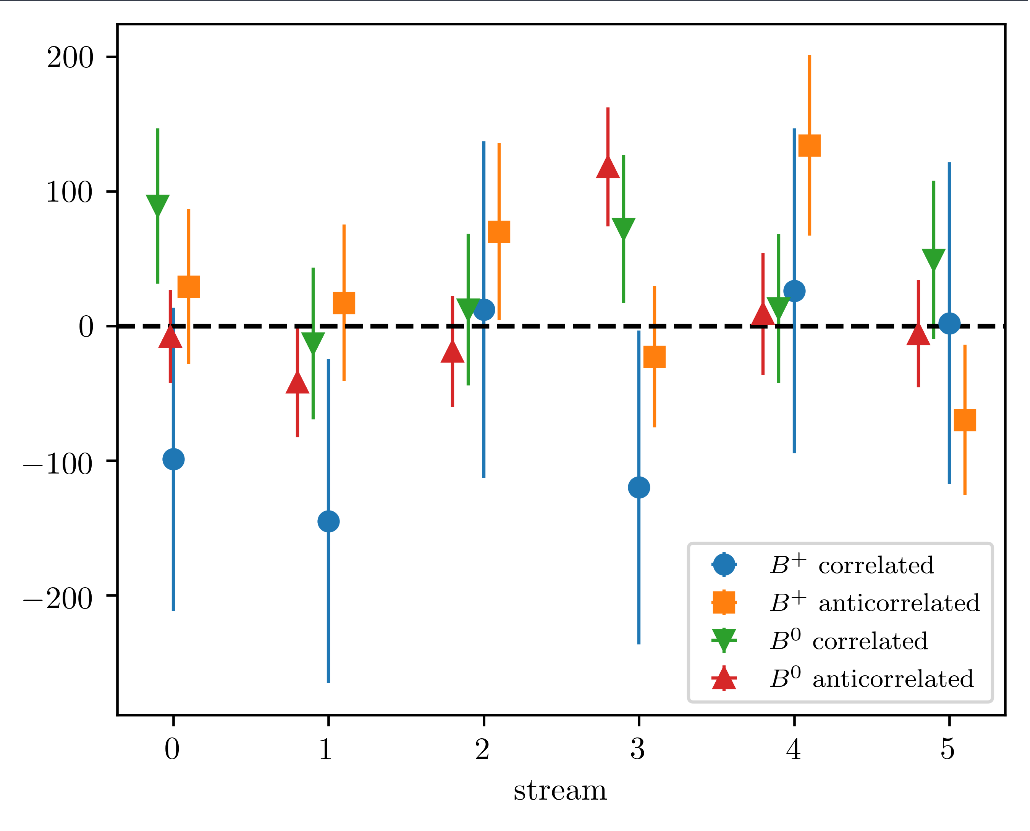
\includegraphics[width=0.85\textwidth]{04-SimultaneousFit/figs/2DsimFitresiduals.png}}
\caption{Residuals of the fitted signal yields resulting from the simultaneous 2D fit by stream and decay mode.}
\label{fig:2DsimFitresiduals}
\end{figure}

Some of the results may seem not well distributed around 0.
 

\begin{figure}[H]
    \centering
    {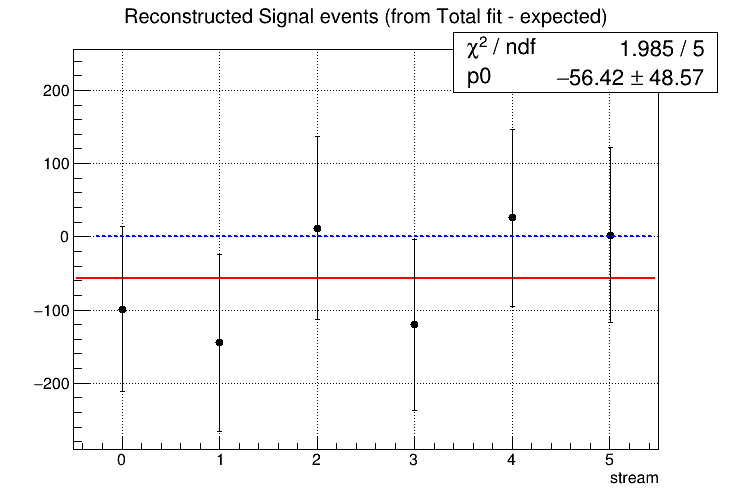
\includegraphics[width=0.85\textwidth]{04-SimultaneousFit/figs/6streamResults_chargedCorrelated_correct.png}}
    \caption{Residuals of the fitted signal yields of charged correlated decays.}
    \label{fig:6streamResults_chargedCorrelated_correct}
    \end{figure}



\newpage

\subsection{toy Monte Carlo study}

For the fit model also toy MC pseudo-experiments were performed in order to confirm the behavior of the fit setup. 
With toy MC experiments the yields, errors and the pulls of the fit are studied by generating our own pseudo-datasets, according to the MC (see plots in
3$\times 10^3$ pseudo-datasets are constructed, where each dataset was generated with the expected amount of events, 
distributed according to the Poisson distribution. Then the composition of each toy pseudo-experiment is fitted as if they were data, and
the pull-value distributions of the fit results are calculated. From the plots showing the  
 pull distributions of the fitted signal yields one can conclude that no bias is present. 
 
 

\begin{figure}[H]
    \centering
    {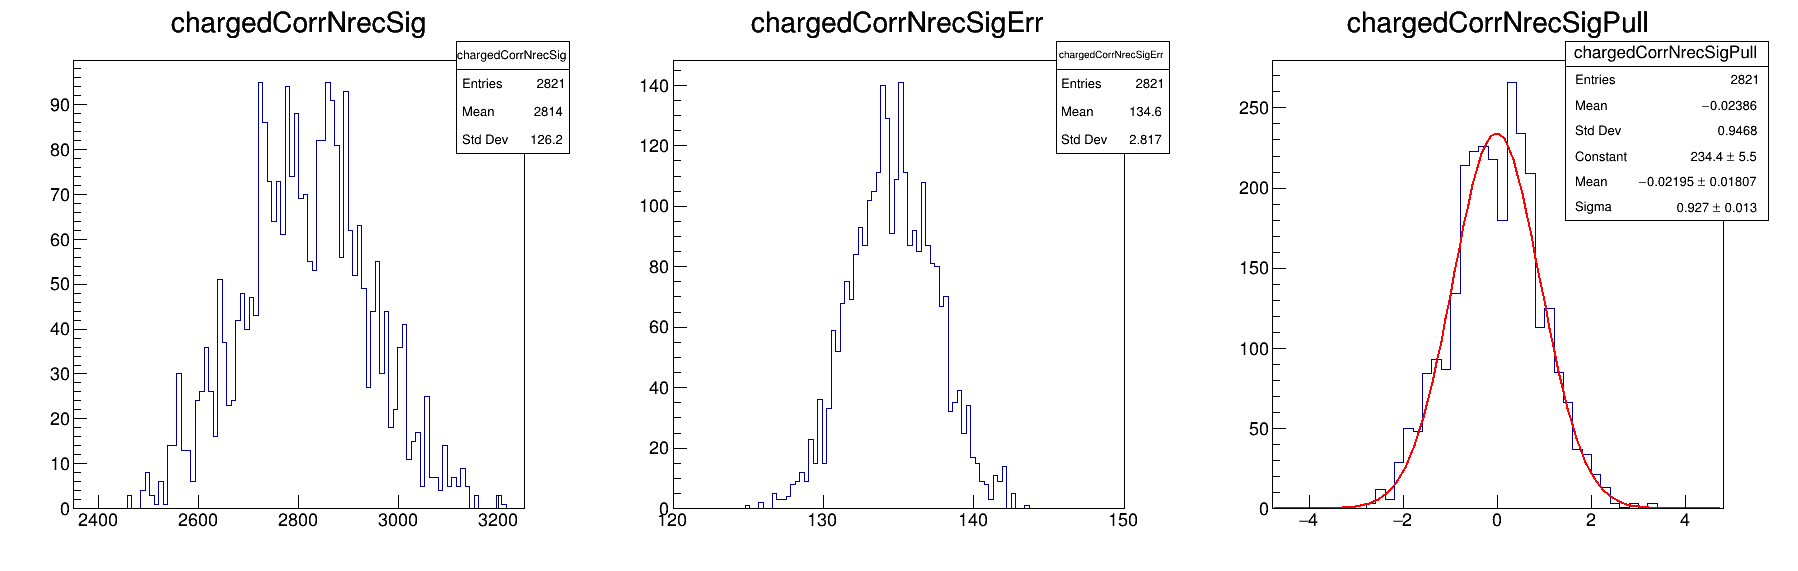
\includegraphics[width=0.85\textwidth]{04-SimultaneousFit/figs/chargedCorrNrecSigPull.png}}
    \caption{Plots showing distributions of the fitted signal yields, errors and the pull
    distribution of all pseudo-fits for the charged correlated decays.}
    \label{fig:2DchargedCorrNrecSigToys}
    \end{figure}


    \begin{figure}[H]
        \centering
        {\includegraphics[width=0.85\textwidth]{04-SimultaneousFit/figs/chargedAntiNrecSigPull.png}}
        \caption{Plots showing distributions of the fitted signal yields, errors and the pull
        distribution of all pseudo-fits for the charged anticorrelated decays.}
        \label{fig:2DchargedAntiNrecSigToys}
        \end{figure}

\begin{figure}[H]
\centering
{\includegraphics[width=0.85\textwidth]{04-SimultaneousFit/figs/neutralCorrNrecSigPull.png}}
\caption{Plots showing distributions of the fitted signal yields, errors and the pull
distribution of all pseudo-fits for the neutral correlated decays.}
\label{fig:2DneutralCorrNrecSigToys}
\end{figure}


\begin{figure}[H]
    \centering
    {\includegraphics[width=0.85\textwidth]{04-SimultaneousFit/figs/neutralAntiNrecSigPull.png}}
    \caption{Plots showing distributions of the fitted signal yields, errors and the pull
    distribution of all pseudo-fits for the neutral anticorrelated decays.}
    \label{fig:2DneutralAntiNrecSigToys}
    \end{figure}
\chapter{$B_{tag}$ fit}

The normalization for the branching fractions is determined from the number of correctly tagged $B$ mesons. 
This value is again determined by fitting the $M_{bc}$ distribution of all $B$ meson candidates tagged
by FEI regardless of the signal side $B$ meson decay.\\
The tagged $B$ meson candidates are selected according to the selection criteria used for the $M_{bc}$ variable  
already illustrated in subsections \crefrange{sec:chargedCorrBtoLambdaC}{sec:neutralAcorrBtoLambdaC}.

%!!! here tell that the Btag samples are selected with same selections as given in selection.tex file. 
% \ref{sec:chargedCorrBtoLambdaC}

\section{Probability Density Functions (PDFs) for the $B_{tag}$}

The reconstructed events can be categorized as follows:
\begin{itemize}
    \item correctly reconstructed $B$ meson candidates: \textbf{reconstructed signal} 
    \item misreconstructed $B$ meson candidates: \textbf{misreconstructed signal}
    \item $B^0$ mesons misreconstructed as $B^+$ (and vice-versa): \textbf{crossfed background} 
    \item and \textbf{continuum background}
\end{itemize}

\subsection{Total Signal fits}\label{sigBtagFit}

As in the 2D fits the total signal is distinguished in \textbf{reconstructed}  and \textbf{misreconstructed signal} depending
on wether it's peaking or not in  $M_{bc}$.\\
\cref{fig:chargedBtag_corrLambdaC_TotalSignalBtag_fit} shows the fit on tagged charged $B$ mesons corresponding to the normalization for the branching fractions of $B^- \rightarrow \Lambda_c^+$ decays.
The $M_{bc}$ distribution of the tagged  $B$ mesons is fitted with a combination of Crystal Ball and Gaussian as for the "peaking" component and the "flat" component is fitted with a Novosibirsk function. 
For the other decay channels instead an Argus function is used to describe the misreconstructed signal (see \crefrange{fig:anticorr_chargedBtag_Total_Signal_fit}{fig:stream0_neutralBtag_anticorrLambdaC_TotalSignal_addedGaussian}).
%Fits show pulls exceeding 3$\sigma$ deviation in some regions, especially in the endpoint region.
%Therefore, in the final fits, the range will be restricted to avoid possible systematic effetcs in the endpoint region.

\begin{figure}[H]
\centering
{\includegraphics[width=0.40\textwidth]{05-BtagFit/figs/chargedBtag_corrLambdaC_TotalSignalBtag_fit.png}}
\caption{Fitted distribution of tagged charged $B$ mesons in the charged correlated decays sample: reconstructed signal events are described by the blue dotted PDF, the misreconstructed with a Novosibirsk function (red dotted). }
\label{fig:chargedBtag_corrLambdaC_TotalSignalBtag_fit}
\end{figure}

\begin{figure}[H]
    \centering
    {\includegraphics[width=0.40\textwidth]{05-BtagFit/figs/stream1_anticorr_chargedBtag_Total_Signal_fit.png}}
    \caption{Fitted distribution of tagged charged $B$ mesons  in the charged anticorrelated decays sample. }
    \label{fig:anticorr_chargedBtag_Total_Signal_fit}
    \end{figure}

\begin{figure}[H]
\centering
{\includegraphics[width=0.40\textwidth]{05-BtagFit/figs/stream0_neutralBtag_corrLambdaC_TotalSignal_addedGaussian.png}}
\caption{Fitted distribution of tagged neutral $B$ mesons reconstructed in neutral correlated decays. }
\label{fig:stream0_neutralBtag_corrLambdaC_TotalSignal_addedGaussian}
\end{figure}

\begin{figure}[H]
\centering
{\includegraphics[width=0.40\textwidth]{05-BtagFit/figs/stream0_neutralBtag_anticorrLambdaC_TotalSignal_addedGaussian.png}}
\caption{Fitted distribution of tagged charged $B$ mesons reconstructed in neutral anticorrelated decays. }
\label{fig:stream0_neutralBtag_anticorrLambdaC_TotalSignal_addedGaussian}
\end{figure}
                        

\subsection{Crossfeed PDF}
 
The crossfeed background is always fitted instead with a sum of a Novosibirsk and an asymmetric Gaussian PDF. 

\begin{figure}[h!]
\centering
{\includegraphics[width=0.40\textwidth]{05-BtagFit/figs/NeutralCrossfeed_stream0_corrLambdaC_chargedBtagFit.png}}
\caption{Crossfeed distribution of charged correlated decays fitted with a sum of Novosibirsk (red) and asymmetric Gaussian PDF (magenta)}
\label{fig:NeutralCrossfeed_stream0_corrLambdaC_chargedBtagFit}
\end{figure}

\begin{figure}[h!]
\centering
{\includegraphics[width=0.40\textwidth]{05-BtagFit/figs/NeutralCrossfeed_stream0_anticorrLambdaC_chargedBtag_MbcFit.png}}
\caption{Crossfeed distribution of charged anticorrelated decays}
\label{fig:NeutralCrossfeed_stream0_corrLambdaC_chargedBtagFit}
\end{figure}

\newpage

\begin{figure}[H]
\centering
{\includegraphics[width=0.40\textwidth]{05-BtagFit/figs/ChargedCrossfeed_stream0_corrLambdaC_neutalBtag_MbcFit.png}}
\caption{Crossfeed distribution of neutral correlated decays}
\label{fig:ChargedCrossfeed_stream0_corrLambdaC_neutalBtag_MbcFit}
\end{figure}

\begin{figure}[H]
\centering
{\includegraphics[width=0.40\textwidth]{05-BtagFit/figs/ChargedCrossfeed_stream0_anticorrLambdaC_neutralBtag_MbcFit.png}}
\caption{Crossfeed distribution  of neutral anticorrelated decays}
\label{fig:ChargedCrossfeed_stream0_anticorrLambdaC_neutralBtag_MbcFit}
\end{figure}

\newpage

\subsection{Continuum PDF}
\noindent  As for the continuum background, a similar procedure as the one described already for the two dimensional fit was adopted:

\begin{itemize}
    \item first the off-resonance sample is scaled accordingly
    \item the ratio between the scaled off-resonance and the on-resonance in MC is calculated in each bin (see Fig.\ref{fig:stream0_chargedBtag_off-on_resonance_correct})
    \item the bin-correction is applied on an independent stream and the scaled and bin-corrected $M_{bc}$ distribution is compared with the on-resonance distribution as shown in Fig.\ref{fig:bin_corrected_stream1_off-resonance_on_stream0_on-resonance}
\end{itemize}
\vspace{0.5cm}
Being the statistics much larger than in the 2D sample, there's no need to remove the continuum suppression cut on the off-resonance sample. 

\begin{figure}[H]
 \centering
\subcaptionbox{\label{fig:stream0_chargedBtag_off-on_resonance_correct}}
{\includegraphics[width=.45\textwidth]{05-BtagFit/figs/stream0_chargedBtag_off-on_resonance_correct.png}}
\subcaptionbox{\label{fig:bin_corrected_stream1_off-resonance_on_stream0_on-resonance}}
{\includegraphics[width=.45\textwidth]{05-BtagFit/figs/bin_corrected_stream1_off-resonance_on_stream0_on-resonance.pdf}} 
\caption{On the left: $M_{bc}$ distributions of the MC off-resonance sample and the MC continuum sample with applied continuum suppression. On the right: $M_{bc}$ distributions of the corrected scaled MC off-resonance and on-resonance MC continuum.}
\end{figure}



\newpage
\section{ $B_{tag}$ fit}\label{BtagFit_onMC}
An independent Monte Carlo stream was used to test the total fit model on tagged $B$ meson candidates.
As in the 2D fit, the parameter for the width, $\sigma_{CB}$, of the Crystal Ball is floated. 
The ratio between expected crossfeed background events and  misreconstructed signal events is fixed from the MC. 
The misreconstructed signal PDF is also not fully constrained: the parameter describing the tail is free. 
To avoid introducing significant systematic uncertainties in the fit deriving from the $M_{bc}$ endpoint region, where one has a smearing effect due to variations of the
beam energy at the MeV level, the range for the fit is restricted to values betweeen 5.250 and 5.287 GeV/c$^2$.


\subsection{Fit results for $B^- \rightarrow \Lambda_c^+$ decays}  


\begin{figure}[H]
    \centering
    {\includegraphics[width=0.50\textwidth]{05-BtagFit/figs/NEW_stream5_chargedBtag_Total_fit_sigmaCB_misReco_Tail_free_370bins.png}}
    \caption{Total fit of tagged $B$ mesons on Monte Carlo simulated data.}
    \label{fig:chargedCorrLambdaC_BtagFit}
    \end{figure}
    \vspace{1.5cm} 

Yields for the reconstructed and misreconstructed signal are obtained from the fit:\\
\vspace{0.25 cm}

\begin{tabular}{ |p{2.5cm}||p{4.2cm}| p{4.2cm}|  }
 \hline
          &    Fit results                 &  expected\\
 \hline
 NrecSig  & 4.7787 $\cdot$10 $^6 \pm$ 6748 &  4.7571 $\cdot$10 $^6 \pm$ 3214 \\
 NmisSig &  5.3987 $\cdot$10 $^6 \pm$ 5617 & 5.4035 $\cdot$10 $^6 \pm$ 3376 \\
 \hline
\end{tabular}

\vspace{0.5 cm}
The normalization for the branching fraction is given by the NrecSig yields. The yields obtained in the fit differ by $\sim 3.2 \sigma$ 
from the expected ones (obtained from a fit to the Total Signal events only).  This discrepancy will impact the final 
measurement.

%The Total Signal (the sum  NrecSig+NmisSig) is 10134027 $\pm$ 4402 (to be compared with 10157950 from the Monte Carlo). 
% This reflects a $\sim 5.5\sigma$ discrepancy between the true MC value and the result from the fit. This can produce some systematic effect, 
 %but the relative error is at the $\sim$ \textperthousand level. 
 %This is still negligible compared to the systematic uncertainity corresponding to the the ${N_{tag}}$ determination, 
 %and furthermore in the branching fraction calculation it is also negligible compared to the statistical uncertainity on 
 %the extracted yields 
%from the two dimensional fit.
 
To check the stability of the fit model a toy MC study was performed with  $3\times10^3$ pseudo-datasets. 
No evidence for possible biases in the reconstructed signal yields was found (see \cref{fig:NrecSignalchargedCorrBtag_mcstudy}).


\begin{figure}[H]
    \centering
    {\centering\includegraphics[width=14cm]{05-BtagFit/figs/NrecSigBtag_mcstudy.png}}
     \caption{Plots showing distributions of the fitted signal yields, errors and the pull distribution of
    all pseudo-fits. (see Appendix \ref{sec:chargedBtoLamApp} for the other free parameters' results)}
      \label{fig:NrecSignalchargedCorrBtag_mcstudy}
      \end{figure}



\subsection{Fit results for $B^- \rightarrow \bar{\Lambda}_c^-$ decays}  
\begin{figure}[H]
    \centering
    {\includegraphics[width=0.50\textwidth]{05-BtagFit/figs/NEW_chargedBtag_anticorrLambdaC_Total_fit_sigmaCB_misRecoSlope_free_370bins.png}}
    \caption{Total fit of tagged $B$ mesons on Monte Carlo simulated data.}
    \label{fig:chargedAntiLambdaC_BtagFit}
    \end{figure}
    \vspace{1.5cm} 


    \begin{tabular}{ |p{2.5cm}||p{4.2cm}|  }
        \hline
        NrecSig  & 2.50831$\cdot$10$^6 \pm$ 11866\\
        NmisSig &  7.37010$\cdot$10$^5 \pm$ 7472 \\
        \hline
       \end{tabular}
       
       
       \vspace{0.5 cm}
       \noindent The Total Signal (the sum  NrecSig+NmisSig) is 3292168 $\pm$ 2423 (to be compared with 3299629 from the Monte Carlo), which means a $\sim 3\sigma$ underestimation. As in the case of charged flavor-correlated decays, this can produce some systematic effect which needs to be taken into account.
       %In fact, a slight underestimation of the Total Signal is found also in the result of the toy Monte Carlo study: \cref{fig:Total_Signal_chargedBtagToyMCstudy} shows the results for the Total Signal events and one can notice a mean value for the pulls consistently below zero.
       
%\begin{figure}[H]
      %  \centering
      %  {\centering\includegraphics[width=14cm]{05-BtagFit/figs/Total_Signal_chargedBtagToyMCstudy.png}}
%\caption{Plots showing distributions of the fitted signal yields, errors and the pull distribution of
     %   all pseudo-fits. (see Appendix \ref{sec:chargedBtoLamApp} for the other free parameters' results)}
     %     \label{fig:Total_Signal_chargedAntiBtagToyMCstudy}
     %     \end{figure}
       
But when performing a toy Monte Carlo study\footnote{as usual performed with  $3\times10^3$ pseudo-datasets} 
the result show no bias on the recosntructed signal yields (see \cref{fig:NrecSig_chargedAntiBtag_mcstudy})


\begin{figure}[H]
    \centering
    {\centering\includegraphics[width=14cm]{05-BtagFit/figs/NrecSig_chargedAntiBtag_mcstudy.png}}
    \caption{Plots showing distributions of the fitted signal yields, errors and the pull distribution of
    all pseudo-fits. }
    \label{fig:NrecSig_chargedAntiBtag_mcstudy}
    \end{figure}
                     


\subsection{Fit results for $\bar{B^0} \rightarrow \Lambda_c^+$ decays} 

\begin{figure}[H]
    \centering
    {\includegraphics[width=0.50\textwidth]{05-BtagFit/figs/neutralCorrLambdaC_BtagFit.png}}
    \caption{Total fit of tagged $B$ mesons on Monte Carlo simulated data.}
    \label{fig:neutralCorrLambdaC_BtagFit}
    \end{figure}
    \vspace{1.5cm} 

Reconstructed and misreconstructed signal yields obtained from the fit:\\
    \vspace{0.25 cm}
    
    \begin{tabular}{ |p{2.5cm}||p{4.2cm}|  }
     \hline
     NrecSig  & 1.7215 $\cdot$10 $^6 \pm$ 3421\\
     NmisSig &  5.5950 $\cdot$10 $^5 \pm$ 2215 \\
     \hline
    \end{tabular}      
    
    \vspace{0.5 cm}
    \noindent The Total Signal (the sum  NrecSig+NmisSig) is 2281033 $\pm$ 1947 (to be compared with 2286964 from the Monte Carlo).
    Also in this case there's a $\sim 3\sigma$ underestimation. 
   
 \vspace{0.5 cm}
       
\begin{figure}[H]
\centering
{\centering\includegraphics[width=14cm]{05-BtagFit/figs/NrecSig_neutralCorrBtag_mcstudy.png}}
\caption{Plots showing distributions of the fitted signal yields, errors and the pull distribution of
all pseudo-fits. }
\label{fig:NrecSig_neutralCorrBtag_mcstudy}
\end{figure}
       

    

\subsection{Fit results for $B^0 \rightarrow \bar{\Lambda}_c^+$ decays} 



\begin{figure}[H]
    \centering
    {\includegraphics[width=0.50\textwidth]{05-BtagFit/figs/stream1_neutralBtag_Total_fit_sigmaCB_misReco_slope_free_370bins.png}}
    \caption{Total fit of tagged $B$ mesons on Monte Carlo simulated data.}
    \label{fig:neutralAntiLambdaC_BtagFit}
    \end{figure}
    \vspace{1.5cm} 

Reconstructed and misreconstructed signal yields obtained from the fit:\\
    \vspace{0.25 cm}
    
    \begin{tabular}{ |p{2.5cm}||p{4.2cm}|  }
     \hline
     NrecSig  & 1.5302 $\cdot$10 $^6 \pm$ 3269\\
     NmisSig &  3.8332 $\cdot$10 $^5 \pm$ 2072 \\
     \hline
    \end{tabular}      
 
   
 \vspace{0.5 cm}
 \noindent The Total Signal (the sum  NrecSig+NmisSig) is 1913476 $\pm$ 1812 (to be compared with 1920156 from the Monte Carlo).
 Also in this case there is an underestimation of about a $\sim 3.7\sigma$. 
 
        
The toy MC study result for the signal yields is shown in \cref{fig:NrecSig_neutralAntiBtag_mcstudy}.
 Also in this case no hints of bias are visible.

\begin{figure}[H]
    \centering
    {\centering\includegraphics[width=14cm]{05-BtagFit/figs/NrecSigneutralAntiBtag_mcstudy.png}}
    \caption{Plots showing distributions of the fitted signal yields, errors and the pull distribution of
    all pseudo-fits. }
    \label{fig:NrecSig_neutralAntiBtag_mcstudy}
    \end{figure}

\chapter{Efficiencies}

Here a decision was made not to rely on the estimated number of $B$ meson pair, as it is usually done, and the absolute FEI efficiency, since the latter shows large discrepancy between MC and data (see i.e. the results reported in the PhD Thesis by M. Gelb \cite{gelb_moritz_2018_21546} and also by J. Schwab \cite{schwab_judith_2017_21422} ) and also it depends strongly on the signal-side (i.e. $\epsilon^{+}_{FEI} \neq \epsilon^{+}_{FEI,  sig}$). 
Instead, to limit the systematics, the branching ratio normalization is obtained using the fitted tagged $B$ mesons and the ratio $\epsilon^{+}_{FEI,  sig} / \epsilon^{+}_{FEI}$ measured on MC, 
which one can expect to be better  described by the MC than the absolute FEI efficiency.
%The final samples contain both signal and background candidates
%from various sources and in order to extract $N_{tag, \Lambda_c} $ and ${N_{tag}}$  unbinned extended maximum-likelihood fits are performed.  \\

\section{FEI Efficiencies}
One needs to distinguish two different FEI efficiencies as already anticipated. \\

The generic FEI efficiency $\epsilon_{FEI} = \frac{n^\circ of tagged B}{total n^\circ of events}$ is the generic efficiency to tag correctly a $B^+B^-$ or $B^0\bar{B^0}$ event, i.e.: 
the hadronic decay-chain of the tag-side $B$ meson is correctly reconstructed, independently from signal-side. The denominator is given by all $B\bar{B}$ events present in the considered sample. 
The generic FEI efficiency is the one that affects the normalization in the branching ratio calculation.\\

The FEI efficiency that affects the numerator of the branching ratio is called signalside-dependent efficiency $\epsilon_{FEI,  sig}$.
In the case one is trying to reconstruct $B^- \rightarrow \Lambda_c^+$ decays, then this efficiency is determined as the follwoing ratio:
$\epsilon^{+}_{FEI,  sig } = \frac{n^\circ of tagged B^{+/-} of B^- \rightarrow \Lambda_c^+}{total n^\circ of B^- \rightarrow \Lambda_c^+ events}$ 

\subsection{Generic FEI efficiency}

The number of correctly tagged $B$ mesons is determined from the yields of reconstructed signal events obtained from a fit
 of the $B_{tag}$ distribustions shown already in   Sec. \ref{sigBtagFit}. As an example \cref{fig:stream5_chargedBtag_TotalSignal_addedGaussian_Normalisations}
 shows the same distributions shown in \cref{fig:chargedBtag_corrLambdaC_TotalSignalBtag_fit} where all shaping parameters have been 
fixed and only the the normalisations of \textbf{reconstructed}  and \textbf{misreconstructed signal} were floated. \\
 %shown in \cref{fig:chargedBtag_corrLambdaC_TotalSignalBtag_fit} in 

 
 \begin{figure}[H]
    \centering
    {\includegraphics[width=0.40\textwidth]{06-Efficiencies/figs/stream5_chargedBtag_TotalSignal_addedGaussian_Normalisations.png}}
    \caption{Fitted distribution of tagged charged B mesons in the charged correlated
    decays sample.}
    \label{fig:stream5_chargedBtag_TotalSignal_addedGaussian_Normalisations}
    \end{figure}

 \subsection{Signalside-dependent FEI efficiency}

 The FEI tag-side efficiency for signal events is calculated upon 10 streams of on-resonance Monte Carlo streams of simulated data 
 in order to minimize statistical uncertainties.
 As an example \cref{fig:10streams_chargedBtag_corrLambdaC_TotalSignalBtag_fit} shows the fit performed on the tagged $B$ mesons having in the ROE a companion decaying $B^- \rightarrow \Lambda_c^+$ (charged correlated decays). 
 Dividing the yields obtained by the fit by the total number of $B^- \rightarrow \Lambda_c^+ events$ present in the 10 streams it is possible to determine the FEI tag-side efficiency for signal events.
 \begin{figure}[H]
    \centering
    {\includegraphics[width=0.40\textwidth]{06-Efficiencies/figs/10streams_chargedBtag_corrLambdaC_TotalSignalBtag_fit.png}}
    \caption{Fit of tagged $B$ mesons in the "signal events" sample}
    \label{fig:10streams_chargedBtag_corrLambdaC_TotalSignalBtag_fit}
    \end{figure}
\section{$\Lambda_c$ efficiency}
The efficiency of reconstructing the ${\Lambda_c}$ baryon after correctly tagging the charged $B$ meson, can be estimated from Monte Carlo simulated data.
All available 10 streams of on-resonance Monte Carlo streams of simulated data were used to minimize statistical uncertainties.
The efficiency is evaluated as follows from the fraction:  
\begin{equation}
    \frac{N_{recSig}(B_{tag}, \Lambda_c)}{N_{recSig}(B_{tag}^{sig})}
\end{equation}

\vspace{0.5cm}

\noindent where $N_{recSig}(B_{tag}, \Lambda_c))$ are the yields of reconstructed signal from a two dimensional fit of corresponding inclusive decay.
 and  $N_{recSig}(B_{tag}^{sig})$ are the yields of correctly reconstructed signal from the same fit of tagged $B$ mesons used to calculate the Signalside-dependent FEI efficiency. 

\subsection{$B^- \rightarrow \Lambda_c^+$ decays}
$\epsilon^+_{FEI,sig} = 0.636 \pm 0.003\%$ (calculated with 10 streams)\\
$\epsilon^+_{FEI} = 0.6379 \pm 0.0004\%$
$\frac{\epsilon^+_{FEI,sig}}{\epsilon^+_{FEI}}$ = 0.997 $\pm $ 0.005% 𝜖𝐹𝐸𝐼,𝑠𝑖𝑔= 0.636 ± 0.003% , 𝜖𝐹𝐸𝐼 = 0.638 ± 0.0004%

$\epsilon_{\Lambda_c}$ = 37.78 $\pm $ 0.45 $\%$ %correction factor: 0.969*0.853*0.983 = 0.813 ± 0.013

\subsection{$B^- \rightarrow \bar{\Lambda}_c^-$ decays}
$\epsilon^+_{FEI,sig} = 0.334 \pm 0.003\%$ (calculated with 10 streams)\\
$\epsilon^+_{FEI} = 0.3461 \pm 0.0002\%$
FEI calculation includes mixed events, $\epsilon_{\Lambda_c}$ is calculated without them
$\frac{\epsilon^+_{FEI,sig}}{\epsilon^+_{FEI}}$ = 0.965 $\pm $ 0.009% 𝜖𝐹𝐸𝐼,𝑠𝑖𝑔 = 0.334 ±0.003%  , 𝜖𝐹𝐸𝐼= 0.346 $\pm$ 0.0002%

$\epsilon_{\Lambda_c}$ = 42.39 $\pm $ 0.66 $\%$ %overall correction factor 0.794 ± 0.010


\subsection{$\bar{B^0} \rightarrow \Lambda_c^+$  decays}
$\epsilon^+_{FEI,sig} = 0.247 \pm 0.002\%$ (calculated with  10 streams unmixed)\\
$\epsilon^+_{FEI} = 0.236 \pm 0.0002\%$ (1 unmixed stream)

$\frac{\epsilon^+_{FEI,sig}}{\epsilon^+_{FEI}}$ = 1.056 $\pm$ 0.010% 𝜖𝐹𝐸𝐼=  0.234 ± 0.001% , 𝜖𝐹𝐸𝐼,𝑠𝑖𝑔= 0.247 ± 0.002%

$\epsilon_{\Lambda_c}$ = 39.59 $\pm $ 0.49 $\%$ %overall correction factor 0.794 $\pm$ 0.010
 (using unmixed events)

\subsection{$\bar{B^0} \rightarrow \Lambda_c^-$  decays}


$\frac{\epsilon^+_{FEI,sig}}{\epsilon^+_{FEI}}$ = 1.005 $\pm$ 0.014% 𝜖𝐹𝐸𝐼= 0.206 ± 0.001% , 𝜖𝐹𝐸𝐼,𝑠𝑖𝑔= 0.207 ± 0.003%

$\epsilon_{\Lambda_c}$ = 41.49  $\pm $ 1.13 $\%$ %overall correction factor 0.790 $\pm$ 0.011
\chapter{Branching ratio}
To measure the inclusive branching fractions

\begin{equation}
    Br(B^{+/-} \rightarrow \Lambda_c^{+} X) = \frac{ N_{tag, \Lambda_c} \cdot  \epsilon^{+}_{FEI}}{N_{tag} \cdot Br(\Lambda_c^+ \rightarrow  p K^- \pi^+) \epsilon_{\Lambda_c} \epsilon^{+}_{FEI,  sig }}
\end{equation}\label{eq:chargedB_BRformula}

\begin{equation}
    Br(B^{0} \rightarrow \Lambda_c^{+/-} X) = \frac{ N_{tag, \Lambda_c} \cdot  \epsilon^{0}_{FEI}}{N_{tag} \cdot Br(\Lambda_c^+ \rightarrow  p K^- \pi^+) \epsilon_{\Lambda_c} \epsilon^{0}_{FEI,  sig }}
\end{equation}\label{eq:B0_BRformula}

the following quantities need to be known: 
\begin{itemize}

\item $N_{tag, \Lambda_c} $ is the reconstructed signal yield obtained from a two dimensional fit of $M_{bc}$ and $M(p K \pi)$ in the final sample.
\item ${N_{tag}}$ is the reconstructed signal yield obtained from the $M_{bc}$ fit of all the tagged $B$ mesons in the final sample.
\item $\epsilon_{\Lambda_c} $ is the $\Lambda_c$ reconstruction efficiency.
\item $\epsilon^{+}_{FEI}$ ($\epsilon^{0}_{FEI}$) represent the hadronic tag-side efficiency for generic $B^+B^- $ ($B^0\bar{B^0}$) events. 
\item $\epsilon^{+}_{FEI,  sig}$ ($\epsilon^{0}_{FEI,  sig }$) represents the hadronic tag-side efficiency for  $B^+B^-$ ($B^0\bar{B^0}$) events where the tagged $B$ meson decays hadronically and the accompanying meson decays inclusively into the studied signal channel. 
\item  $Br(\Lambda_c^+ \rightarrow  p K^- \pi^+) $: the branching fraction of the decay mode used to reconstruct the  $\Lambda_c$ baryon.
\end{itemize}
\vspace{0.2 cm}


\begin{table}[H]
    \centering
    \resizebox{0.95\textwidth}{!}{%
    \setlength{\tabcolsep}{8pt}
    \begin{tabular}{c c c c c c c}
    
    \toprule
     \hline
         &  total fit \hspace{0.5 cm}  & signal fit  &  BELLE MC VALUE  \\
     \midrule
     \hline
    stream 0	&	(2.84 $\pm$ 0.13)$\%$  &	(2.96 $\pm$ 0.07)$\%$	 &	(2.91 $\pm$ 0.03)$\%$\\
    stream 1	&	(2.82 $\pm$ 0.14)$\%$	&	(2.99 $\pm$ 0.07)$\%$	 &	(2.91 $\pm$ 0.03)$\%$	\\
    stream 2	&	(2.97 $\pm$ 0.14)$\%$	&	(2.97 $\pm$ 0.07)$\%$	 &	(2.90 $\pm$ 0.03)$\%$\\
    stream 3	&	(2.76 $\pm$ 0.14)$\%$	&	(2.90 $\pm$ 0.07)$\%$	 &	(2.91 $\pm$ 0.03)$\%$\\
    stream 4	&	(3.06 $\pm$ 0.14)$\%$ &	    (3.05 $\pm$ 0.07)$\%$	 &	(2.90 $\pm$ 0.03)$\%$\\
    stream 5	&	(2.83 $\pm$ 0.14)$\%$	&	(2.84 $\pm$ 0.07)$\%$	 &	(2.92 $\pm$ 0.03)$\%$\\
    \midrule
    \hline
    average			&	(2.88 $\pm$	0.06)$\%$	&	(2.95 $\pm$	0.03)$\%$	& (2.91 $\pm$ 0.01)$\%$\\
    \bottomrule
    \hline
    \end{tabular}%
    }
    \label{tab:SixStreams_chargedCorrLamBR}
    \caption{charged corr}
    %\caption{Measured branching fraction values obtained using the results listed in \cref{tab:SixStreams_chargedCorrLam2Dfits} for the six different streams (only statistical uncertainties are displayed) and its average.}
    \end{table}

    \begin{table}[H]
        \centering
        \resizebox{0.95\textwidth}{!}{%
        \setlength{\tabcolsep}{8pt}
        \begin{tabular}{c c c c c c c}
        
        \toprule
         \hline
             &  total fit \hspace{0.5 cm}  & signal fit  &  BELLE MC VALUE  \\
         \midrule
         \hline
        stream 0	&	(1.24 $\pm$ 0.11)$\%$  &	(1.19 $\pm$ 0.05)$\%$	 &	(1.217 $\pm$ 0.002)$\%$\\
        stream 1	&	(1.24 $\pm$ 0.11)$\%$	&	(1.21 $\pm$ 0.05)$\%$	 &	(1.218 $\pm$ 0.002)$\%$	\\
        stream 2	&	(1.35 $\pm$ 0.12)$\%$	&	(1.23 $\pm$ 0.05)$\%$	 &	(1.218 $\pm$ 0.002)$\%$\\
        stream 3	&	(1.16 $\pm$ 0.10)$\%$	&	(0.20 $\pm$ 0.05)$\%$	 &	(1.215 $\pm$ 0.002)$\%$\\
        stream 4	&	(1.44 $\pm$ 0.13)$\%$   &	(1.21 $\pm$ 0.05)$\%$	 &	(1.218 $\pm$ 0.002)$\%$\\
        stream 5	&	(1.04 $\pm$ 0.11)$\%$	&	(1.15 $\pm$ 0.05)$\%$	 &	(1.217 $\pm$ 0.002)$\%$\\
        \midrule
        \hline
        average		&	(1.25 $\pm$	0.05)$\%$	&	(1.20 $\pm$	0.02)$\%$	& (1.217 $\pm$ 0.001)$\%$\\
        \bottomrule
        \hline
        \end{tabular}%
        }
    \label{tab:SixStreams_chargedAntiCorrLamBR}
    \caption{charged anticorr}
    %\caption{Measured branching fraction values obtained using the results listed in \cref{tab:SixStreams_chargedCorrLam2Dfits} for the six different streams (only statistical uncertainties are displayed) and its average.}
    \end{table}

\section{extraction of neutral decays branching fractions}
Due to the mixing phenomenon of neutral $B$ mesons the measurement requires an intermediate step in order to correct the production 
obtained rates of $\Lambda_c$ baryons in the reocoil of the reconstructed neutral $B$ mesons for the $B^0\bar{B^0}$ mixing. \\
Being $\chi_d$ the mixing parameters, on average, if one looks at the recoil of a correctly reconstructed $B^0$ ($\bar{B^0}$) meson $1 - \chi_d$ of the time the reconstructed $\Lambda_c$ baryon
will have decayed from a $\bar{B^0}$ ($B^0$) and $\chi_d$ of the time from $B^0$ ($\bar{B^0}$), due to mixing.\\

i.e.:   
\begin{equation}
    \begin{cases}
        \mathcal{B}(B^0_{tag}, \Lambda_c^-) = (1 - \chi_d) \mathcal{B}_c + \chi_d \bar{\mathcal{B}}_c \\

        \mathcal{B}(\bar{B}^0_{tag}, \Lambda_c^-) = (1 - \chi_d) \bar{\mathcal{B}}_c + \chi_d \mathcal{B}_c
    \end{cases}  
\end{equation}

are the two equations corresponding to the spurious correlated/ anticorrelated branching ratios, with  $\chi_d$ factor of missing events
and $\chi_d$ amount of events that belong actually to the other type of decays. Solving those simultaneous equations one obtains the
mixing-corrected branching ratios $\mathcal{B}_c$ (correlated decays) and $\bar{\mathcal{B}}$ (anticorrelated decays): \\

\begin{equation}
    \begin{cases}
        \mathcal{B}_c  = \dfrac{\mathcal{B}(B^0_{tag}, \Lambda_c^-) - \chi_d (\mathcal{B}(B^0_{tag}, \Lambda_c^-) +  \mathcal{B}(\bar{B}^0_{tag}, \Lambda_c^-))}{1 - 2\chi_d}      \\

        \bar{\mathcal{B}}_c = \dfrac{(\bar{B}^0_{tag}, \Lambda_c^-) - \chi_d (\bar{B}^0_{tag}, \Lambda_c^-) +  \mathcal{B}(B^0_{tag}, \Lambda_c^-))}{1 - 2\chi_d}
    \end{cases}  
\end{equation}
\\
First a check of the decays that didn't experience mixing is performed.
\subsection{unmixed neutral decays branching ratios}

\begin{table}[H]
    \centering
    \resizebox{0.65\textwidth}{!}{%
    \setlength{\tabcolsep}{8pt}
    \begin{tabular}{c c c}
    
    \toprule
     \hline
         &    signal fit  &  BELLE MC VALUE  \\
     \midrule
     \hline
    stream 0	&	(3.48 $\pm$ 0.11)$\%$	 &	(3.439 $\pm$ 0.003)$\%$\\
    stream 1	&	(3.54 $\pm$ 0.11)$\%$	 &	(3.431 $\pm$ 0.003)$\%$	\\
    stream 2	&	(3.48 $\pm$ 0.11)$\%$	 &	(3.433 $\pm$ 0.003)$\%$\\
    stream 3	&	(3.47 $\pm$ 0.11)$\%$	 &	(3.433 $\pm$ 0.003)$\%$\\
    stream 4	&	(3.34 $\pm$ 0.11)$\%$	 &	(3.434 $\pm$ 0.003)$\%$\\
    stream 5	&	(3.45 $\pm$ 0.11)$\%$	 &	(3.436 $\pm$ 0.003)$\%$\\
    \midrule
    \hline
    average			&	(3.46 $\pm$	0.05)$\%$	& (3.434 $\pm$ 0.001)$\%$\\
    \bottomrule
    \hline
    \end{tabular}%
    }
    \caption{Measured branching fraction values obtained using only unmixed events for the six different streams (only statistical uncertainties are displayed) and its average.}
    \end{table}
    


    \begin{table}[H]
        \centering
        \resizebox{0.65\textwidth}{!}{%
        \setlength{\tabcolsep}{8pt}
        \begin{tabular}{c c c}
        
        \toprule
         \hline
             &    signal fit  &  BELLE MC VALUE  \\
         \midrule
         \hline
        stream 0	&	(1.35 $\pm$ 0.09)$\%$	 &	(1.300 $\pm$ 0.002)$\%$\\
        stream 1	&	(1.30 $\pm$ 0.07)$\%$	 &	(1.299 $\pm$ 0.002)$\%$	\\
        stream 2	&	(1.31 $\pm$ 0.07)$\%$	 &	(1.300 $\pm$ 0.002)$\%$\\
        stream 3	&	(1.31 $\pm$ 0.07)$\%$	 &	(1.299 $\pm$ 0.002)$\%$\\
        stream 4	&	(1.22 $\pm$ 0.09)$\%$	 &	(1.295 $\pm$ 0.002)$\%$\\
        stream 5	&	(1.30 $\pm$ 0.07)$\%$	 &	(1.298 $\pm$ 0.002)$\%$\\
        \midrule
        \hline
        average			&	(1.30 $\pm$	0.03)$\%$	& (1.299 $\pm$ 0.001)$\%$\\
        \bottomrule
        \hline
        \end{tabular}%
        }
        \caption{Measured branching fraction values obtained using only unmixed events for the six different streams (only statistical uncertainties are displayed) and its average.}
        \end{table}    

\section{Systematics}


\subsection{Continuum background}\label{sec:continuumSysBtoLambdaC}

2 sources of systematics:
\begin{itemize}
\item difference in the shapes 
\item different impact of the Continuum Suppression cut
\end{itemize}

To estimate the first type of uncertainty two-dimensional fits with varied parameters' values by their uncertainties 
(a fit with $+$err and $-$err) were performed. \\
The rescaling procedure used to model the on-resonance continuum distribution is far from perfect, especially in the case of the $B_{tag}$ fit.
As one can see from \cref{fig:stream5_chargedBtag_Total_fit}:
\\
\begin{figure}[H]
    \centering
    \subcaptionbox{\label{fig:stream5_chargedBtag_Total_fit}}
    {\includegraphics[width=.65\textwidth]{07-LamBR/figs/stream5_chargedBtag_Total_fit.png}} 
    \subcaptionbox{\label{fig:stream5_chargedBtag_TotalFit_TrueContinuum}}
    {\includegraphics[width=.65\textwidth]{07-LamBR/figs/NEW_stream5_chargedBtag_Total_fit_sigmaCB_misReco_Tail_free_usingTrueContinuumPDF_370bins.png}} 
    \caption{Above: Fitted $M_{bc}$ of charged correlated decays with scaled off-resonance continuum distribution. 
    Below: same $M_{bc}$ distribution with the true continuum distribution.}
    \end{figure}
  
The bumps visible for  $M_{bc} < 5.27 GeV/c^2$ in \cref{fig:stream5_chargedBtag_Total_fit}   
are a consequence of the imperfect scaling procedure used to model the continuum background. In fact, 
they disappear completely (in \cref{fig:stream5_chargedBtag_TotalFit_TrueContinuum} ) when the same fit is performed using 
the pdf obtained directly from the on-resonance distribution (\cref{fig:stream5_chargedBtag_continuumHistPdf})
There is a significant impact on the fit results, the values from the  $B_{tag}$ fit in the charged correlated channel are reported here below:

\begin{table}[H]
    \begin{tabular}{ |p{2.5cm}||p{4.5cm}| p{4.5cm}| }
    \hline
        \    &  Fit with scaled continuum &  Fit with true continuum\\
     \hline
     $N_{recSig}$  yields     &  $4.7787  \cdot 10^6 \pm 6.75 \cdot 10^3 $   & $ 4.7474  \cdot 10^6 \pm 8.01 \cdot 10^3$\\
   
     \hline
    \end{tabular}
    \caption{Signal yields obtained in $B_{tag}$ fits shown in \cref{fig:stream5_chargedBtag_Total_fit} and \cref{fig:stream5_chargedBtag_TotalFit_TrueContinuum}.}
    \end{table}
    \vspace{0.2 cm}

The yields are to be compared with the values obtained when fitting the total signal distribution shown
in \cref{fig:chargedBtag_corrLambdaC_TotalSignalBtag_fit}: $N_{recSig} = 4.7571  \cdot 10^6 \pm 3.23 \cdot 10^3$.
The continuum modeling alone is responsible for a discrepancy of about 3.2$\sigma$ on the yields.
This discrepancy and the impact on the branching fraction are accounted in the systematic uncertainties derived from the continuum modeling. 
This source of systematics is responsible for 0.02 $\%$ uncertainty on the branching ratio.
\begin{figure}
    \centering
    {\includegraphics[width=0.5\textwidth]{07-LamBR/figs/stream5_chargedBtag_continuumHistPdf.png}}
    \caption{$M_{bc}$ on-resonance MC distribution of charged correlated decays.}
    \label{fig:stream5_chargedBtag_continuumHistPdf}
    \end{figure}
The other type of systematic uncertainty in modeling the continuum is originated by the continuum suppression cut having a slightly different efficiency on data (as a consequence of the shift in off-resonance MC and data visible in the the $foxWolframR2$ distribution in Fig. \ref{fig:R2_MC-Data_off_resonance_distributions}). 
As already discussed, it originates a possible  discrepancy of about 2.25$\%$ in continuum background events in the two dimensional fit (and only 1.25$\%$  in the $B_{tag}$ fit). The statistical uncertainty on this fraction of events can also be taken into account as systematics. 
Being the number of events in the off-resonance data sample without the continuum suppression applied is very small, the uncertainty in the mentioned fraction of events is negligible compared to the statistical uncertainty on the on-resonance continuum background events in MC: it would account for 0.002$\%$ on the BR value. 
Therefore, this second source of uncertainty is not taken into account.
There would be also a third of systematic uncertainty given by potential difference in the on-/off-resonance correction between data and MC, but there's no way one can estimate it properly.


\subsection{Crossfeed ratio}\label{sec:CrossfeedRatioSysBtoLambdaC}
The ratio crossfeed/misreconstructed signal is kept fixed in the $B_{tag}$ fit to the MC value.
 This choice was made according to the fact that the two categories of events have  
a similar origin: in both cases the $B$ mesons were not correctly reconstructed, either because of missing or wrongly added particles 
(misreconstructed signal events) or, in the case of crossfeed events because the tagged $B$ meson was not the required
 one ($B^0$ meson instead of a $B^{+/-}$ meson). 
The ratio between these two categories of events is therefore expected to be very similar in MC and data, 
though there's no guarantee that the efficiency to reconstruct them is the same in data in data and consequently 
the above mentioned ratios could differ on data. Unfortunately there's no direct way to have an estimate of the possible 
discrepancy for them.\\  
In \cite{gelb_moritz_2018_21546} (and previously in \cite{schwab_judith_2017_21422}) it was found that there's a substantial 
difference in terms of tagging efficiency for FEI applied on Monte Carlo and on Belle data, being the discrepancy around $\sim$ 20$\%$. 
We can assume that the efficiency for the two categories of events on data will both differ of that value and the ratio of the events 
being the same MC value, but in absence of any other method to estimate the uncertainty on it one can consider a maximal 
discrepancy of 20$\%$ between Monte Carlo and data to study the impact on the yields\footnote{This method was also validated 
with the control decay sample and the originated uncertainty is well within the PDG reported ones.}. 

\subsection{Crossfeed $B_{tag}$ PDF}
Since also the shapes of the PDFs decribing the crossfeed background in the $B_{tag}$ fit are fully fixed to the
ones determined with the limited Monte Carlo statistics, also their statistical uncertainties
need to be taken into account as possible source of systematics.
To estimate this source of uncertainty fits with varied parameters' values by their uncertainties 
(a fit with $+$err and $-$err) were performed.

\subsection{2DFit crossfeed normalization}
As discussed in the 2D simulateous fit section, in each decay channel the normalization of crossfeed events 
is estimated using the fitted reconstructed signal events of the corresponding crossfeeding channel in the as follows:
\begin{equation}
N_{cross } = N_{recSig}^{correlated} (\dfrac{\epsilon_{cross}}{\epsilon_{recSig}})^{correlated} + 
N_{recSig}^{anticorrelated} (\frac{\epsilon_{cross}}{\epsilon_{recSig}})^{anticorrelated}
\end{equation}
where  $\epsilon_{recSig}$  and $\epsilon_{cross}$ are respectively the efficiency to reconstruct correctly
 signal events in the crossfeeding channel and the efficiency of reconstructing those events as crossfeed in the
 channel of interest.\\
 The uncertainties of those two efficiencies may cause an overestimation or underestimation of the crossfeed 
 in the channel of interest. To estimate the systematic uncertainty deriving from it, the simultaneous fits 
 have been performed modifying the ratio of the efficiencies by the respective uncertainties maximising the shift, 
 i.e. using $\frac{\epsilon_{cross} + \sigma}{\epsilon_{recSig} - \sigma}$ and $\frac{\epsilon_{cross} - \sigma}{\epsilon_{recSig} + \sigma}$ 

 \subsection{2DFit $M_{bc}$ peaking/flat PDFs}
As discussed in \cref{sec:MC2D_Fit} the shapes of the PDFs describing the generic background (peaking or flat in $M_{bc}$ ) are kept fixed
 in the two dimensional fit. This source of systematics is handled in the same way as the crossfeed background in the $B_{tag}$:
 fits with varied parameters' values by their uncertainties were performed (procedure is repeated for $M_{bc}$ peaking and flat background).

 \subsection{PID  efficiency correction}\label{sec:chargedCorrPIDcorrSys}

 The PID selection efficiency for the three charged particles in the signal decay needs
 to be corrected on MC due to various differences, when comparing to data. The
 Belle PID group has prepared a set of correction factors and tables of systematic
 uncertainties for PID efficiencies for all charged particles.
 %The PID efficiency in data is usually lower in data than in Monte Carlo simulations, therefore the efficiency of reconstructing $\Lambda_c$ baryons needs to be corrected accordingly when calculating the branching fraction on data, taking into account the PID corrections corresponding to each of the hadrons in which it decays\footnote{since on all of them a PID selection cut is applied}. \\
 The proton identification efficiency was studied in \cite{PIDeff}.
 The inclusive $\Lambda^0$ decay $\Lambda^0 \rightarrow p \pi^-$   was used to examine the proton identification efficiency difference between data 
 and MC in \textit{Belle}. The datasets for the SVD1 and SVD2 periods are treated separately, and the efficiency ratio dependence on proton charge, 
 momentum and polar angle is considered. The study is done for the proton ID cut values 0.6, 0.7, 0.8 and 0.9\footnote{Here, proton ID cut value $X$ means $  \mathcal{L}_{p/K} > X$ and $  \mathcal{L}_{p/\pi} > X$}. 
 The binning on the momentum starts at 0.2 GeV. 
 The proton ID efficiency is defined as\\
 \vspace{0.2cm}
 \newline
 \hspace{3 cm}    $\epsilon_{PID} = \frac{\text{number of}\hspace{0.05 cm}p \text{tracks identified as} \hspace{0.05 cm} p}{\text{number of }p \hspace{0.05 cm} \text{tracks} }$\\
 
 \vspace{0.2cm}
  and the comparison between MC efficiency and data efficiency by a double ratio defined as \\
 
 \vspace{0.2cm} \hspace{1 cm}  $ R_p = \epsilon^{data}/\epsilon^{MC}$ \\
 
 \vspace{0.5cm}
 \noindent The average proton ID correction is estimated to be: \hspace{0.5 cm} $R_p = 0.969 \pm 0.003$.
 
 \vspace{0.2 cm}
 \noindent  The kaon identification efficiency was studied in detail in Belle Note 779 \cite{KIDeff} (\url{http://belle.kek.jp/secured/belle_note/gn779/bn779.ps.gz}). The decay $D^{*+} \rightarrow D^0 \pi^+$ followed by $D^0 \rightarrow K^- \pi^+$, was used to examine it. As for the proton identification efficiency it considers the dependence on Kaon charge, momentum and polar angle and same ID cut values\footnote{Here, Kaon ID cut value $X$ means $  \mathcal{L}_{K/\pi} > X$, so for values below $X$ the tracks are identified as pions} 

\subsection{$B^- \rightarrow \Lambda_c^+$ decays}
Regarding the systematic uncertainties deriving from the continuum modeling in the two-dimensional fit are estimated as 
already described in \ref{continuumSysBtoLambdaC} one obtains an absolute value of $0.04\%$ on the branching fraction.\\
Instead the imperfect modeling of the continuum in the $B_{tag}  $ fit is responsible for a 0.02 $\%$ on the branching fraction in absolute value.\\
Continuum modeling uncertainties account for 0.05$\%$ total uncertainties on the branching fraction in absolute value.
\vspace{1 cm}

To estimate the systematics derived from the crossfeed/misreconstructed signal ratio, in the $B_{tag}$ fit the number of crossfeed events 
were varied artificially in order to have $\pm$20$\%$ different ratio, keeping the previosuly determined Monte Carlo ratio fixed.

\vspace{0.25 cm}
\begin{table}[H]
\begin{tabular}{ |p{2.5cm}||p{2cm}| p{2cm}|  p{2cm}|}
\hline
       &  $- \sigma$ &  $+ \sigma$ & $ \pm \bar{\sigma}$\\
 \hline
 offset    &  20010 &  9330 & 14670 \\
 \hline
\end{tabular}
\caption{Offsets on the $N_{recSig}$  signal yields obtained varying of $\pm$20$\%$ the 
 ratio of crossfeed/misreconstructed events in the $B_{tag}$ fit and mean deviations reported in the last column.}
\end{table}

The offsets that a potential $\pm$20$\%$ different crossfeed/misreconstructed signal ratio produce results in 0.01$\%$ systematic
uncertainity on the branching fraction.
\\
The systematic uncertainties deriving from the crossfeed background modeling in the $B_{tag}$ fit is estimated following 
the same procedure  described for continuum modeling systematics in the two dimensional fit.\\
In the table below the signal yields' offsets are listed changing
the parameters within their uncertainties, and the mean offsets value used to calculate the
expected uncertainty on the BR value. The resulting absolute systematic uncertainty is
about 0.01$\%$ on the BR value.
\vspace{0.25 cm}
\begin{table}[H]
\begin{tabular}{ |p{2.5cm}||p{2cm}| p{2cm}|  p{2cm}|}
\hline
       &  $- \sigma$ &  $+ \sigma$ & $ \pm \bar{\sigma}$\\
 \hline
 offset    &  14810 &  17280 & 16045 \\
 \hline
\end{tabular}
\caption{Offsets on the $N_{recSig}$  signal yields  obtained varying the parameters of crossfeed
background PDFs within their uncertainties in the $B_{tag}$ fit and mean
deviations reported in the last column. }
\end{table}

\begin{table}[h]
    \centering
    \resizebox{0.8\textwidth}{!}{%
    \begin{tabular}{c c c}
    \hline
    source              & relative ($\%$) & absolute ($\%$)  \\
    \hline
    Continuum modeling   &  1.77   &  0.05 \\
    $B_{tag}$ fit Crossfeed fraction   &  0.35 &  0.01 \\
    $B_{tag}$ fit Crossfeed PDF shape & 0.35 &  0.01  \\
    2DFit crossfeed normalization & 0.70 & 0.02 \\
    $M_{bc}$ peaking PDF shape & 0.35 &  0.01  \\
    $M_{bc}$ flat PDF shape & 0.35 &  0.01 \\
    
    $\epsilon^{+}_{FEI,  sig}/\epsilon^{+}_{FEI}$ & 0.35 & 0.01 \\
    $\epsilon_{\Lambda_c}$ & 1.41 & 0.04 \\
    PID            & 1.75    & 0.05 \\
    Tracking efficiency & 0.35  & 0.01 \\
    \hline
    Total                         &   3.18     &  0.09  \\
    \hline
    \end{tabular}%
    }%
    \caption{Systematic uncertainties in the determination of the  $B^+ \rightarrow \bar{\Lambda}_c^- X$ branching fraction in \si{\percent}.}
    \label{tab:systematics:ChargedCorr}
    \end{table}
    

    \subsection{$B^+ \rightarrow \Lambda_c^+$ decays}

    Regarding the systematic uncertainties deriving from the continuum modeling in the two-dimensional fit are estimated 
    one obtains an absolute value of $0.02\%$ on the branching fraction.\\
%%!TEX root = ../main.tex
\clearpage

{\noindent\bf\Huge Appendices}
\addcontentsline{toc}{section}{Appendix}
\appendix


%chargedCorrBtoLambdaPlots
%!TEX root = ../main.tex
%

\subsection{$B^- \rightarrow \Lambda_c^+$ decays: additional plots}
%\section{$B^- \rightarrow \Lambda_c^+$ decays: additional plots}%\label{}
\label{sec:chargedBtoLamApp}



\begin{figure}[H]
  \begin{subfigure}{15cm}
    \centering\includegraphics[width=14cm]{A1-Appendix/figs/Signal_window_streams12345_Generic_charged_corrLambdaC_2Dfit.png}
   % \caption{Fit on $M(p K \pi)$ in the region $5.25 < M_{bc} < 5.258$ GeV/c$^2$.  }
   % \label{fig:CrossfeedMbcRegionsInvMpeak1}
  \end{subfigure}
  \begin{subfigure}{15cm}
    \centering\includegraphics[width=14cm]{A1-Appendix/figs/Mbc_Sideband_stream12345_Generic_charged_corrLambdaC_2Dfit.png}
  \end{subfigure}

  \begin{subfigure}{15cm}
    \centering\includegraphics[width=14cm]{A1-Appendix/figs/InvM_Sideband_stream12345_Generic_charged_corrLambdaC_2Dfit.png}
  \end{subfigure}
  \caption{Signal region and sidebands of the two dimensional fit of generic background shown in \cref{fig:5streams_Generic_charged_corrLambdaC_2Dfit}}
\end{figure}


\newpage


\begin{figure}[H]
  \begin{subfigure}{15cm}
    \centering\includegraphics[width=14cm]{A1-Appendix/figs/Mbc_Sideband_stream12345_Crossfeed_charged_corrLambdaC_2Dfit_afterParametrization.png}
   % \caption{Fit on $M(p K \pi)$ in the region $5.25 < M_{bc} < 5.258$ GeV/c$^2$.  }
   % \label{fig:CrossfeedMbcRegionsInvMpeak1}
  \end{subfigure}
  \begin{subfigure}{15cm}
    \centering\includegraphics[width=14cm]{A1-Appendix/figs/Signal_window_stream12345_Crossfeed_charged_corrLambdaC_2Dfit_afterParametrization.png}
  \end{subfigure}

  \begin{subfigure}{15cm}
    \centering\includegraphics[width=14cm]{A1-Appendix/figs/InvM_Sideband_stream12345_Crossfeed_charged_corrLambdaC_2Dfit.png}
  \end{subfigure}
  \caption{Signal region and sidebands of the two dimensional fit of crossfeed background after parametrization}
\end{figure}

\newpage


\begin{figure}[H]
  \begin{subfigure}{15cm}
    \centering\includegraphics[width=14cm]{A1-Appendix/figs/Signal_window_stream3_Continuum_charged_corrLambdaC_2Dfit.png}
   % \caption{Fit on $M(p K \pi)$ in the region $5.25 < M_{bc} < 5.258$ GeV/c$^2$.  }
   % \label{fig:CrossfeedMbcRegionsInvMpeak1}
  \end{subfigure}
  \begin{subfigure}{15cm}
    \centering\includegraphics[width=14cm]{A1-Appendix/figs/Mbc_Sideband_stream3_Continuum_charged_corrLambdaC_2Dfit.png}
  \end{subfigure}

  \begin{subfigure}{15cm}
    \centering\includegraphics[width=14cm]{A1-Appendix/figs/InvM_Sideband_stream3_Continuum_charged_corrLambdaC_2Dfit.png}
  \end{subfigure}
  \caption{Signal region and sidebands of the two dimensional fit of continuum background shown in \cref{fig:stream3corrLambddaC_total_continuum_2DFit}}
\end{figure}




\newpage

\begin{figure}[h!]
%\centering
{\includegraphics[width=0.75\textwidth]{A1-Appendix/figs/Signal_window_Total_2DFit_stream0_free_sigmas_free_sigmas.png}}
\caption{Signal region ($2.22 < M(p K \pi) < 2.35$ GeV/c$^2$ and $5.27 < M_{bc} < 5.29$ GeV/c$^2$ ) projections pf the dimensional fit on stream 0 Monte Carlo simulated data.}
\label{fig:stream0_sig_window_Total2Dfit_charged_corrLambdaC}
\end{figure}

\begin{figure}[h!]
%\centering
{\includegraphics[width=0.75\textwidth]{A1-Appendix/figs/Mbc_Sideband_Total_2DFit_stream0_free_sigmas.png}}
\caption{Sideband region of $5.25 < M_{bc} < 5.265$ GeV/c$^2$ projection of the two dimensional fit on stream 0 Monte Carlo simulated data.}
\label{fig:stream0_MbcSideband_Total2Dfit_charged_corrLambdaC}
\end{figure}

\begin{figure}[b]
%\centering
{\includegraphics[width=0.75\textwidth]{A1-Appendix/figs/InvM_Sideband_Total_2DFit_stream0_free_sigmas.png}}
\caption{Sideband region of $2.22 < M(p K \pi) < 2.35$ GeV/c$^2$ projection of the two dimensional fit on stream 0 Monte Carlo simulated data.}
\label{fig:stream0_InvMSideband_Total2Dfit_charged_corrLambdaC}
\end{figure}

\newpage

\begin{figure}[h!]
  \begin{subfigure}{15cm}
    \centering\includegraphics[width=14cm]{A1-Appendix/figs/NrecSigBtag_mcstudy.png}
   % \caption{Fit on $M(p K \pi)$ in the region $5.25 < M_{bc} < 5.258$ GeV/c$^2$.  }
   % \label{fig:CrossfeedMbcRegionsInvMpeak1}
  \end{subfigure}
  \begin{subfigure}{15cm}
    \centering\includegraphics[width=14cm]{A1-Appendix/figs/nMisSig_mcstudy.png}
  \end{subfigure}

  \begin{subfigure}{15cm}
    \centering\includegraphics[width=14cm]{A1-Appendix/figs/sigmaCB_mcstudy.png}
  \end{subfigure}
  \begin{subfigure}{15cm}
    \centering\includegraphics[width=14cm]{A1-Appendix/figs/k_mcstudy.png}
    %\label{fig:CrossfeedMbcRegionsInvMpeak5}
  \end{subfigure}
  %\label{fig:CrossfeedMbcRegionsInvMpeak}
  \caption{Toy MC study for the $B_{tag}$ fit model described in Sec. \ref{BtagFit}}
\end{figure}


\clearpage
%chargedCorrBtoDPlots
%!TEX root = ../main.tex
%

%\section{$B^- \rightarrow D^0$ decays: additional plots}
\subsection{$B^- \rightarrow D^0$ decays: additional plots}
\label{chargedBtoD0App}

Figures \ref{fig:chargedBtoD_FOMvsR2_cut}-\ref{fig:chargedBtoD_FOMvsSigProb_cut} show the FOM values at various cuts 
on $foxWolframR2$ and SignalProbability variables respectively. After the cuts on the first two variables were optimized, the cut on $D^0_{CMS}$ is chosen 
considering the momenta distributions plotted on \ref{fig:chargedcorrD0_Pcms}: $p^{D^0 }_{CMS} > 1$ GeV/c$^2$ removes 
a good portion of background events while retaining most of the signal events.

\begin{figure}[H]
  %\centering
  {\includegraphics[width=0.75\textwidth]{A2-Appendix/figs/R2Optimisation_chargedB_D0Sample.png}}
  \caption{Figure of Merit values calculated at several cuts on the $foxWolframR2$ variable.}
  \label{fig:chargedBtoD_FOMvsR2_cut}
  \end{figure}
   


\begin{figure}[H]
    %\centering
    {\includegraphics[width=0.75\textwidth]{A2-Appendix/figs/SigProbOptimisation_chargedB_D0Sample.png}}
    \caption{Figure of Merit values calculated at several cuts on the SignalProbability variable.}
    \label{fig:chargedBtoD_FOMvsSigProb_cut}
\end{figure}

\begin{figure}[H]
  %\centering
{\includegraphics[width=0.75\textwidth]{A2-Appendix/figs/chargedBtoD0bar_Pcms_afterOpt.png}}
\caption{Distribution of  $D^0$ candidates momenta in the center of mass system after the cuts on $foxWolframR2$ 
and SignalProbability variables were applied.}
\label{fig:chargedcorrD0_Pcms}
\end{figure}
   

Figures \ref{fig:stream0Signal_window_chargedControlD0_Total_2DFit}-\ref{fig:InvM_Sideband_Total_2DFit_stream0} show the projections of signal regions and sidebands in $ M_{bc}$ and in the $D^0$ invariant mass of the two dimensional fit on stream 0.

\begin{figure}[H]
%\centering
{\includegraphics[width=0.75\textwidth]{A2-Appendix/figs/stream0Signal_window_chargedControlD0_Total_2DFit.png}}
\caption{Signal region ( $1.85 < M(\pi K) < 1.88$ GeV/c$^2$ and $5.27 < M_{bc} < 5.29$ GeV/c$^2$) projections of the two dimensional fit on stream0 (\cref{fig:stream0_chargedControlD0_Total_2DFit}).}
\label{fig:stream0Signal_window_chargedControlD0_Total_2DFit}
\end{figure}
 

  \begin{figure}[H]
%\centering
{\includegraphics[width=0.75\textwidth]{A2-Appendix/figs/Mbc_Sideband_Total_2DFit_stream0_free_sigmas.png}}
\caption{Sideband region of $5.25 < M_{bc} < 5.265$ GeV/c$^2$ projection in $M(\pi K)$  of the two dimensional fit on stream 0.}
\label{fig:Mbc_Sideband_Total_2DFit_stream0}
\end{figure}
 
 \begin{figure}[H]
%\centering
{\includegraphics[width=0.75\textwidth]{A2-Appendix/figs/InvM_Sideband_Total_2DFit_stream0_free_sigmas.png}}
\caption{Sideband region of $1.8 < M(\pi K) < 1.84$ GeV/c$^2$ projection in $M_{bc}$ of the two dimensional fit on stream 0. }
\label{fig:InvM_Sideband_Total_2DFit_stream0}
\end{figure}

\crefrange{fig:Signal_window_chargedControlD0_Total_2DFit_onData_free_sigmaCB1_InvMsigma}{fig:InvMsideband_chargedControlD0_Total_2DFit_onData_free_sigmaCB1_InvMsigma} show the projections in $ M_{bc}$ and in the $D^0$ invariant mass of the two dimensional fit on data.

%\begin{figure}[h!]
%\centering
%{\includegraphics[width=0.50\textwidth]{A2-Appendix/figs/chargedControlD0_Generic_Mbc_SideBand_InvM.png}}
%\caption{projection of the sideband $M_{bc} < 5.26 GeV/c^2 $ region of the two dimensional fit shown in \cref{fig:chargedControlD0_Generic_2DFit} for generic background.}
%\label{fig:chargedControlD0_Generic_Mbc_5.26range_InvM}
%\end{figure}



 \begin{figure}[h!]
%\centering
{\includegraphics[width=0.75\textwidth]{A2-Appendix/figs/Signal_window_chargedControlD0_Total_2DFit_onData_free_sigmaCB1_InvMsigma.png}}
\caption{Signal region ( $1.85 < M(\pi K) < 1.88$ GeV/c$^2$ and $5.27 < M_{bc} < 5.29$ GeV/c$^2$) projections of the two dimensional fit on data described in \cref{chargedBtoD0_2Dfit_onData}}
\label{fig:Signal_window_chargedControlD0_Total_2DFit_onData_free_sigmaCB1_InvMsigma}
\end{figure}
 

  \begin{figure}[h!]
%\centering
{\includegraphics[width=0.75\textwidth]{A2-Appendix/figs/Mbc_sideband_chargedControlD0_Total_2DFit_onData_free_sigmaCB1_InvMsigma.png}}
\caption{Sideband region of $5.25 < M_{bc} < 5.265$ GeV/c$^2$ projection in $M(\pi K)$  of the two dimensional fit on data}
\label{fig:Mbc_sideband_chargedControlD0_Total_2DFit_onData_free_sigmaCB1_InvMsigma}
\end{figure}
 
 \begin{figure}[h!]
%\centering
{\includegraphics[width=0.75\textwidth]{A2-Appendix/figs/InvMsideband_chargedControlD0_Total_2DFit_onData_free_sigmaCB1_InvMsigma.png}}
\caption{Sideband region of $1.8 < M(\pi K) < 1.84$ GeV/c$^2$ projection in $M_{bc}$ of the two dimensional fit on data. }
\label{fig:InvMsideband_chargedControlD0_Total_2DFit_onData_free_sigmaCB1_InvMsigma}
\end{figure}

\clearpage
%chargedCorrBtoLambdaPlots
%!TEX root = ../main.tex
%

\subsection{$B^- \rightarrow \bar{\Lambda_c}^-$ decays: additional plots}
%\section{$B^- \rightarrow \Lambda_c^+$ decays: additional plots}%\label{}
\label{sec:chargedAnticorrApp}

\begin{figure}[H]
  \begin{subfigure}{14.5cm}
    \centering\includegraphics[width=13.8cm]{A3-Appendix/figs/2DanticorrLambdaC_NrecSig_mcstudy.png}
   % \caption{Fit on $M(p K \pi)$ in the region $5.25 < M_{bc} < 5.258$ GeV/c$^2$.  }
   % \label{fig:CrossfeedMbcRegionsInvMpeak1}
  \end{subfigure}
  \begin{subfigure}{14.5cm}
    \centering\includegraphics[width=13.8cm]{A3-Appendix/figs/2DanticorrLambdaC_NmisSig_mcstudy.png}
  \end{subfigure}
 
  \begin{subfigure}{14.5cm}
    \centering\includegraphics[width=13.8cm]{A3-Appendix/figs/2DanticorrLambdaC_N_Generic_mcstudy.png}
  \end{subfigure}
  \begin{subfigure}{14.5cm}
    \centering\includegraphics[width=13.8cm]{A3-Appendix/figs/2DanticorrLambdaC_sigmaCB1_mcstudy.png}
  \end{subfigure}
  \begin{subfigure}{14.5cm}
    \centering\includegraphics[width=13.8cm]{A3-Appendix/figs/2DanticorrLambdaC_InvMsigma_mcstudy.png}
    %\label{fig:CrossfeedMbcRegionsInvMpeak5}
  \end{subfigure}
  %\label{fig:CrossfeedMbcRegionsInvMpeak}
  \caption{Toy MC study for the two dimensional fit model described in Sec.  \ref{sec:chargedAnticorr2DtotalFit}}
\end{figure}



\begin{figure}[h!]
%\centering
{\includegraphics[width=0.75\textwidth]{A3-Appendix/figs/Signal_window_Total_2DFit_stream0_chargedAnticorrLambdaC_Crossfeed_fraction.png}}
\caption{Signal region ($2.22 < M(p K \pi) < 2.35$ GeV/c$^2$ and $5.27 < M_{bc} < 5.29$ GeV/c$^2$ ) projections of the dimensional fit on stream 0 Monte Carlo simulated data.}
\label{fig:stream0_sig_window_Total2Dfit_charged_anticorrLambdaC}
\end{figure}

\begin{figure}[h!]
%\centering
{\includegraphics[width=0.75\textwidth]{A3-Appendix/figs/Mbc_Sideband_Total_2DFit_stream0_chargedAnticorrLambdaC_Crossfeed_fraction.png}}
\caption{Sideband region of $5.25 < M_{bc} < 5.265$ GeV/c$^2$ projection of the two dimensional fit on stream 0 Monte Carlo simulated data.}
\label{fig:stream0_MbcSideband_Total2Dfit_charged_anticorrLambdaC}
\end{figure}

\begin{figure}[b]
%\centering
{\includegraphics[width=0.75\textwidth]{A3-Appendix/figs/InvM_Sideband2_Total_2DFit_stream0_chargedAnticorrLambdaC_Crossfeed_fraction.png}}
\caption{Sideband region of $2.22 < M(p K \pi) < 2.35$ GeV/c$^2$ projection of the two dimensional fit on stream 0 Monte Carlo simulated data.}
\label{fig:stream0_InvMSideband_Total2Dfit_charged_anticorrLambdaC}
\end{figure}

\newpage

\begin{figure}[h!]
  \begin{subfigure}{15cm}
    \centering\includegraphics[width=14cm]{A3-Appendix/figs/NrecSigchargedBtag_mcstudy.png}
   % \caption{Fit on $M(p K \pi)$ in the region $5.25 < M_{bc} < 5.258$ GeV/c$^2$.  }
   % \label{fig:CrossfeedMbcRegionsInvMpeak1}
  \end{subfigure}
  \begin{subfigure}{15cm}
    \centering\includegraphics[width=14cm]{A3-Appendix/figs/NmisSigchargedBtag_mcstudy.png}
  \end{subfigure}

  \begin{subfigure}{15cm}
    \centering\includegraphics[width=14cm]{A3-Appendix/figs/sigmaCBchargedBtag_mcstudy.png}
  \end{subfigure}
  \begin{subfigure}{15cm}
    \centering\includegraphics[width=14cm]{A3-Appendix/figs/cArg_chargedBtag_mcstudy.png}
    %\label{fig:CrossfeedMbcRegionsInvMpeak5}
  \end{subfigure}
  %\label{fig:CrossfeedMbcRegionsInvMpeak}
  \caption{Toy MC study for the $B_{tag}$ fit model described in Sec. \ref{sec:chargedAnticorrBtagFit}}
\end{figure}





\clearpage
\addcontentsline{toc}{section}{References}
\setboolean{inbibliography}{true}
\bibliographystyle{belle2-note}
\bibliography{99-References/bibliography}

\end{document}
